\chapter{Neutral Current Event Selection}
\label{ch:Selection}

The NC disappearance analysis is performed by comparing the observed FD spectrum of NC events to the predicted number of events after extrapolation. This requires a largely pure sample of NC signal events. There are three main backgrounds for this sample, $\nue$ CC interactions, $\numu$ CC interactions, and cosmic ray events. This chapter describes the full process for selecting a sample of NC events and eliminating backgrounds, briefly discussing data quality and event quality metrics, and fully detailing the fiducial, containment, NC selection, and cosmic rejection.

The analysis specific cuts were chosen based on the official SA files. These files were produced in tag R16-03-03, and NuS group specific DeCAF files were produced in tag S16-04-08. The cuts were trained on cosmic data from the cosmic trigger so that the actual cosmic prediction could come from the NuMI timing sideband. Beam events were oscillated assuming three flavor oscillations with the parameters listed in Table \ref{tab:3FlavParams}. For normalization simplicity, only 14 diblock MC and data were studied. After applying this criterion, all beam spectra were scaled to \pot{6}, and the cosmic spectra were scaled to $120\unit{s}$. The remainder of this note describes each level of event cut and the data/MC comparison spectra from the ND as validation.
\begin{table}[h]
  \begin{center}
    \caption[Assumed Oscillation Parameters]{The three flavor oscillation parameters assumed for studying the NC selection cuts}
    \label{tab:3FlavParams}
    \begin{tabular}{c c}
      \hline\hline
      Oscillation Parameter & Value \\
      \hline
      $\rho$ & $2.84\unit{g/cm\textsuperscript{3}}$ \\
      $\Delta m^2_{21}$ & $7.53 \times 10^{-5}\evsq$ \\
      $\sin^2 2\theta_{12}$ & $0.846$ \\
      $\Delta m^2_{32}$ & $2.40 \times 10^{-3}\evsq$ \\
      $\theta_{23}$ & $\pi/4$ \\
      $\sin^2 2\theta_{13}$ & $0.084$ \\
      $\delta$ & $0$ \\
      \hline
    \end{tabular}
  \end{center}
\end{table}

\section{Data Quality}

Data quality cuts were developed well before the first \nova~results to ensure proper data taking conditions, and all analysis groups apply them as standard. These cuts are applied per spill, and spills that fail these cuts are not included in POT accounting. The cuts can be categorized into three main groups, beam quality, data quality, and timing.

The beam quality cuts were studied and set as described in ref.~\cite{ref:TNBeamQual}. These cuts ensure that the data was collected during acceptable conditions by cutting on metrics such as the beam position on the target, and the horn current. To be included, spills must meet all of the criteria listed in Table \ref{tab:BeamQual}.
\begin{table}[h]
  \begin{center}
    \caption[Beam Quality Cuts]{Beam quality cuts applied to each spill to ensure proper data taking conditions. Taken from ref.~\cite{ref:TNBeamQual}.}
    \label{tab:BeamQual}
    \begin{tabular}{c c c}
      \hline\hline
      Beam Quality Parameter & Minimum & Maximum \\
      \hline
      Spill POT & $2.00 \times 10^{12}$ & \\
      Horn Current & $-202\unit{kA}$ & $-198\unit{kA}$ \\
      Beam X and Y position on target & $0.02\unit{mm}$ & $2.00\unit{mm}$ \\
      Beam X and Y width & $0.57\unit{mm}$ & $1.58\unit{mm}$ \\
      Time to nearest beam spill & & $0.5\unit{s}$ \\
      \hline
    \end{tabular}
  \end{center}
\end{table}

Two data quality cuts were applied to data from each detector. These cuts were motivated and set as described in \cite{ref:DQND, ref:DQFDDCMLiveGeo, ref:DQFDDCMEdgeFrac}, and are summarized in Table \ref{tab:DataQual}. The ND observes a higher level of noise when lights are on in the detector hall, so a cut is placed on one of the particularly noisy DCMs. Also at the ND, data is only considered good if all of the DCMs are active. A similar cut at the FD is made, but as the detector conditions were changing during commissioning, the cut is made using the LiveGeometry package that properly handles a changing detector. The other cut applied at the FD is an `edge metric' that looks for tracks matching across DCM boundaries and cuts spills where the fraction of matches is too low, cutting spills where the DCMs were out of sync relatively to one another.
\begin{table}[h]
  \begin{center}
    \caption[Data Quality Cuts]{Data quality cuts applied to each spill to ensure proper data taking conditions.}
    \label{tab:DataQual}
    \begin{tabular}{c c c}
      \hline\hline
      Data Quality Parameter & Detector & Metric for Spill to Pass \\
      \hline
      Number of Missing DCMs & ND & $= 0$ \\
      Lights On Effect Hit Fraction & ND & $\leq 0.45$ \\
      Missing DCMs from LiveGeometry & FD & $= 0$ \\
      DCM Edge Match Fraction & FD & $> 0.2$ \\
      \hline
    \end{tabular}
  \end{center}
\end{table}

Finally, a timing cut is applied to cosmic data to ensure that the data is not too close to the edge of the data taking window. For cosmic events within a given $500\,\mu s$ trigger window, only events between $25\,\mu{\mbox{s}} < t < 475\,\mu{\mbox{s}}$ are kept.

Table \ref{tab:NP1DataQual} shows the number of events that pass these data quality cuts, and fig.~\ref{fig:NP1DataQual} shows the energy spectra at the ND and FD.
\begin{table}[h]
  \begin{center}
    \caption[Event Table: Data Quality Cuts]{The number of events that pass the data quality cuts, at both detectors.}
    \label{tab:NP1DataQual}
    \begin{tabular}{c c c c c}
      \hline\hline
      Cut Level & NC & $\numu$ CC & $\nue$ CC & Cosmic \\
      \hline
      \multicolumn{5}{l}{FD:} \\
      Data Quality & 194.8 & 107.3 & 54.0 & 66148.4 \\
      \multicolumn{5}{l}{ND $(\times 10^{3})$:} \\
      Data Quality & 3934 & 13904 & 246 & \\
      \hline
    \end{tabular}
  \end{center}
\end{table}

\begin{figure}[h]
  \centering
  \begin{subfigure}{.48\textwidth}
    \centering
    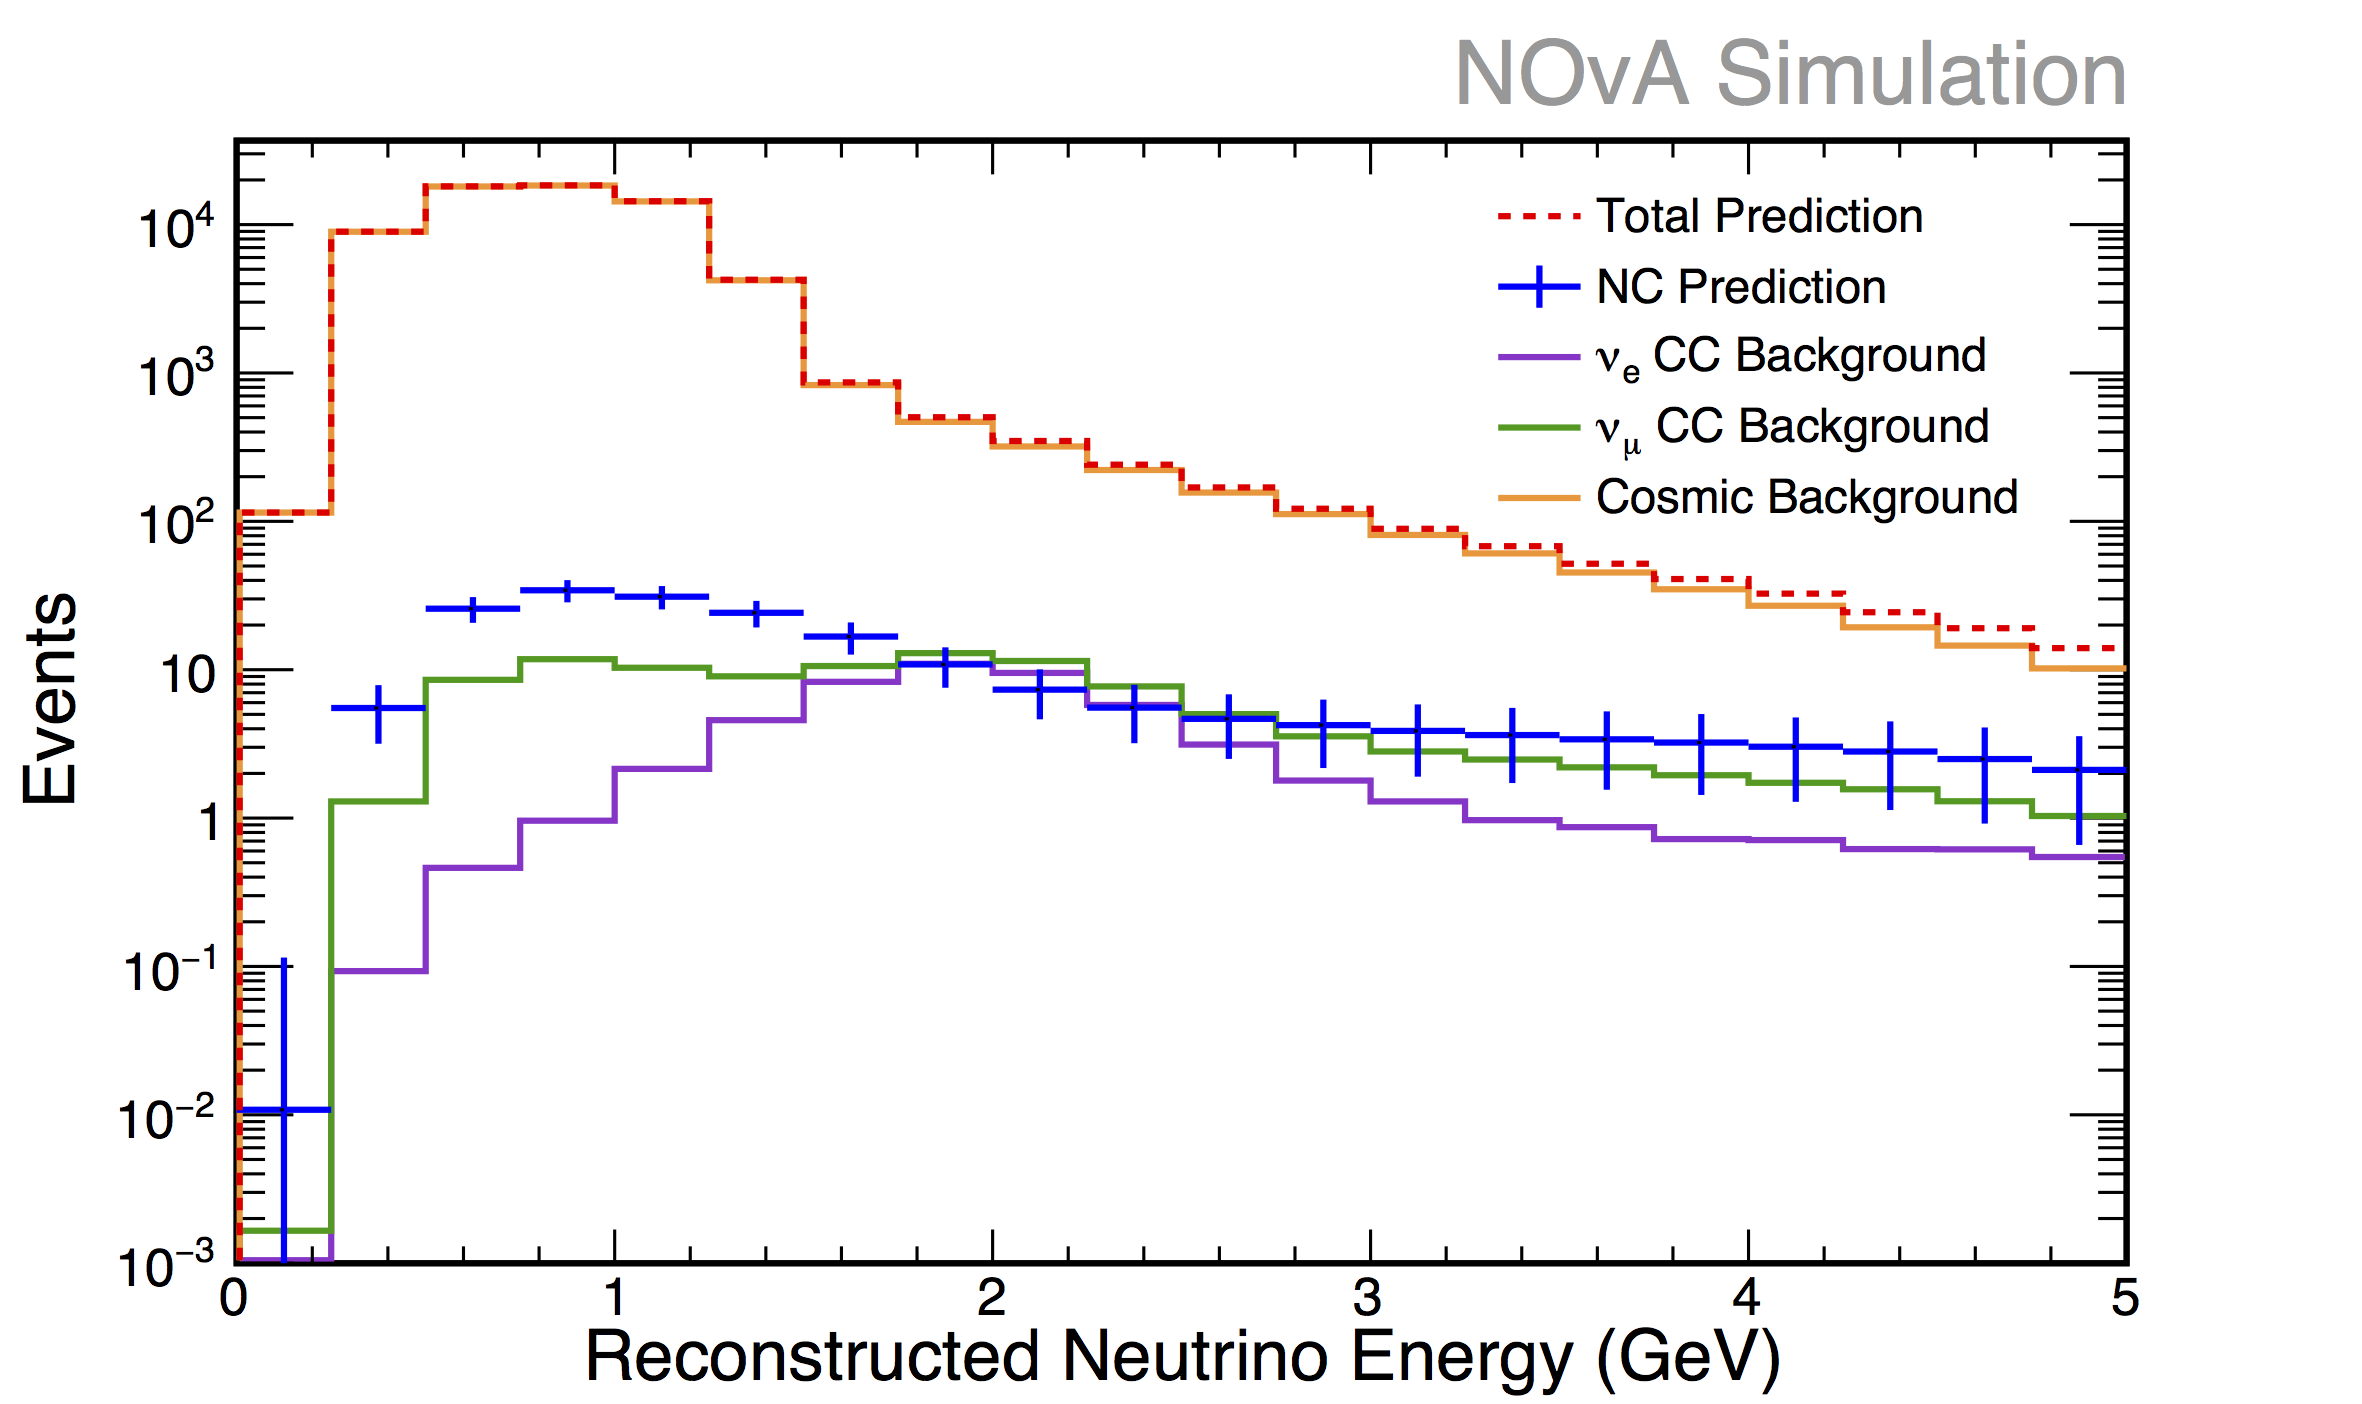
\includegraphics[width=1\linewidth]{figures/RecoE0FD.png}
  \end{subfigure}
  \begin{subfigure}{.48\textwidth}
    \centering
    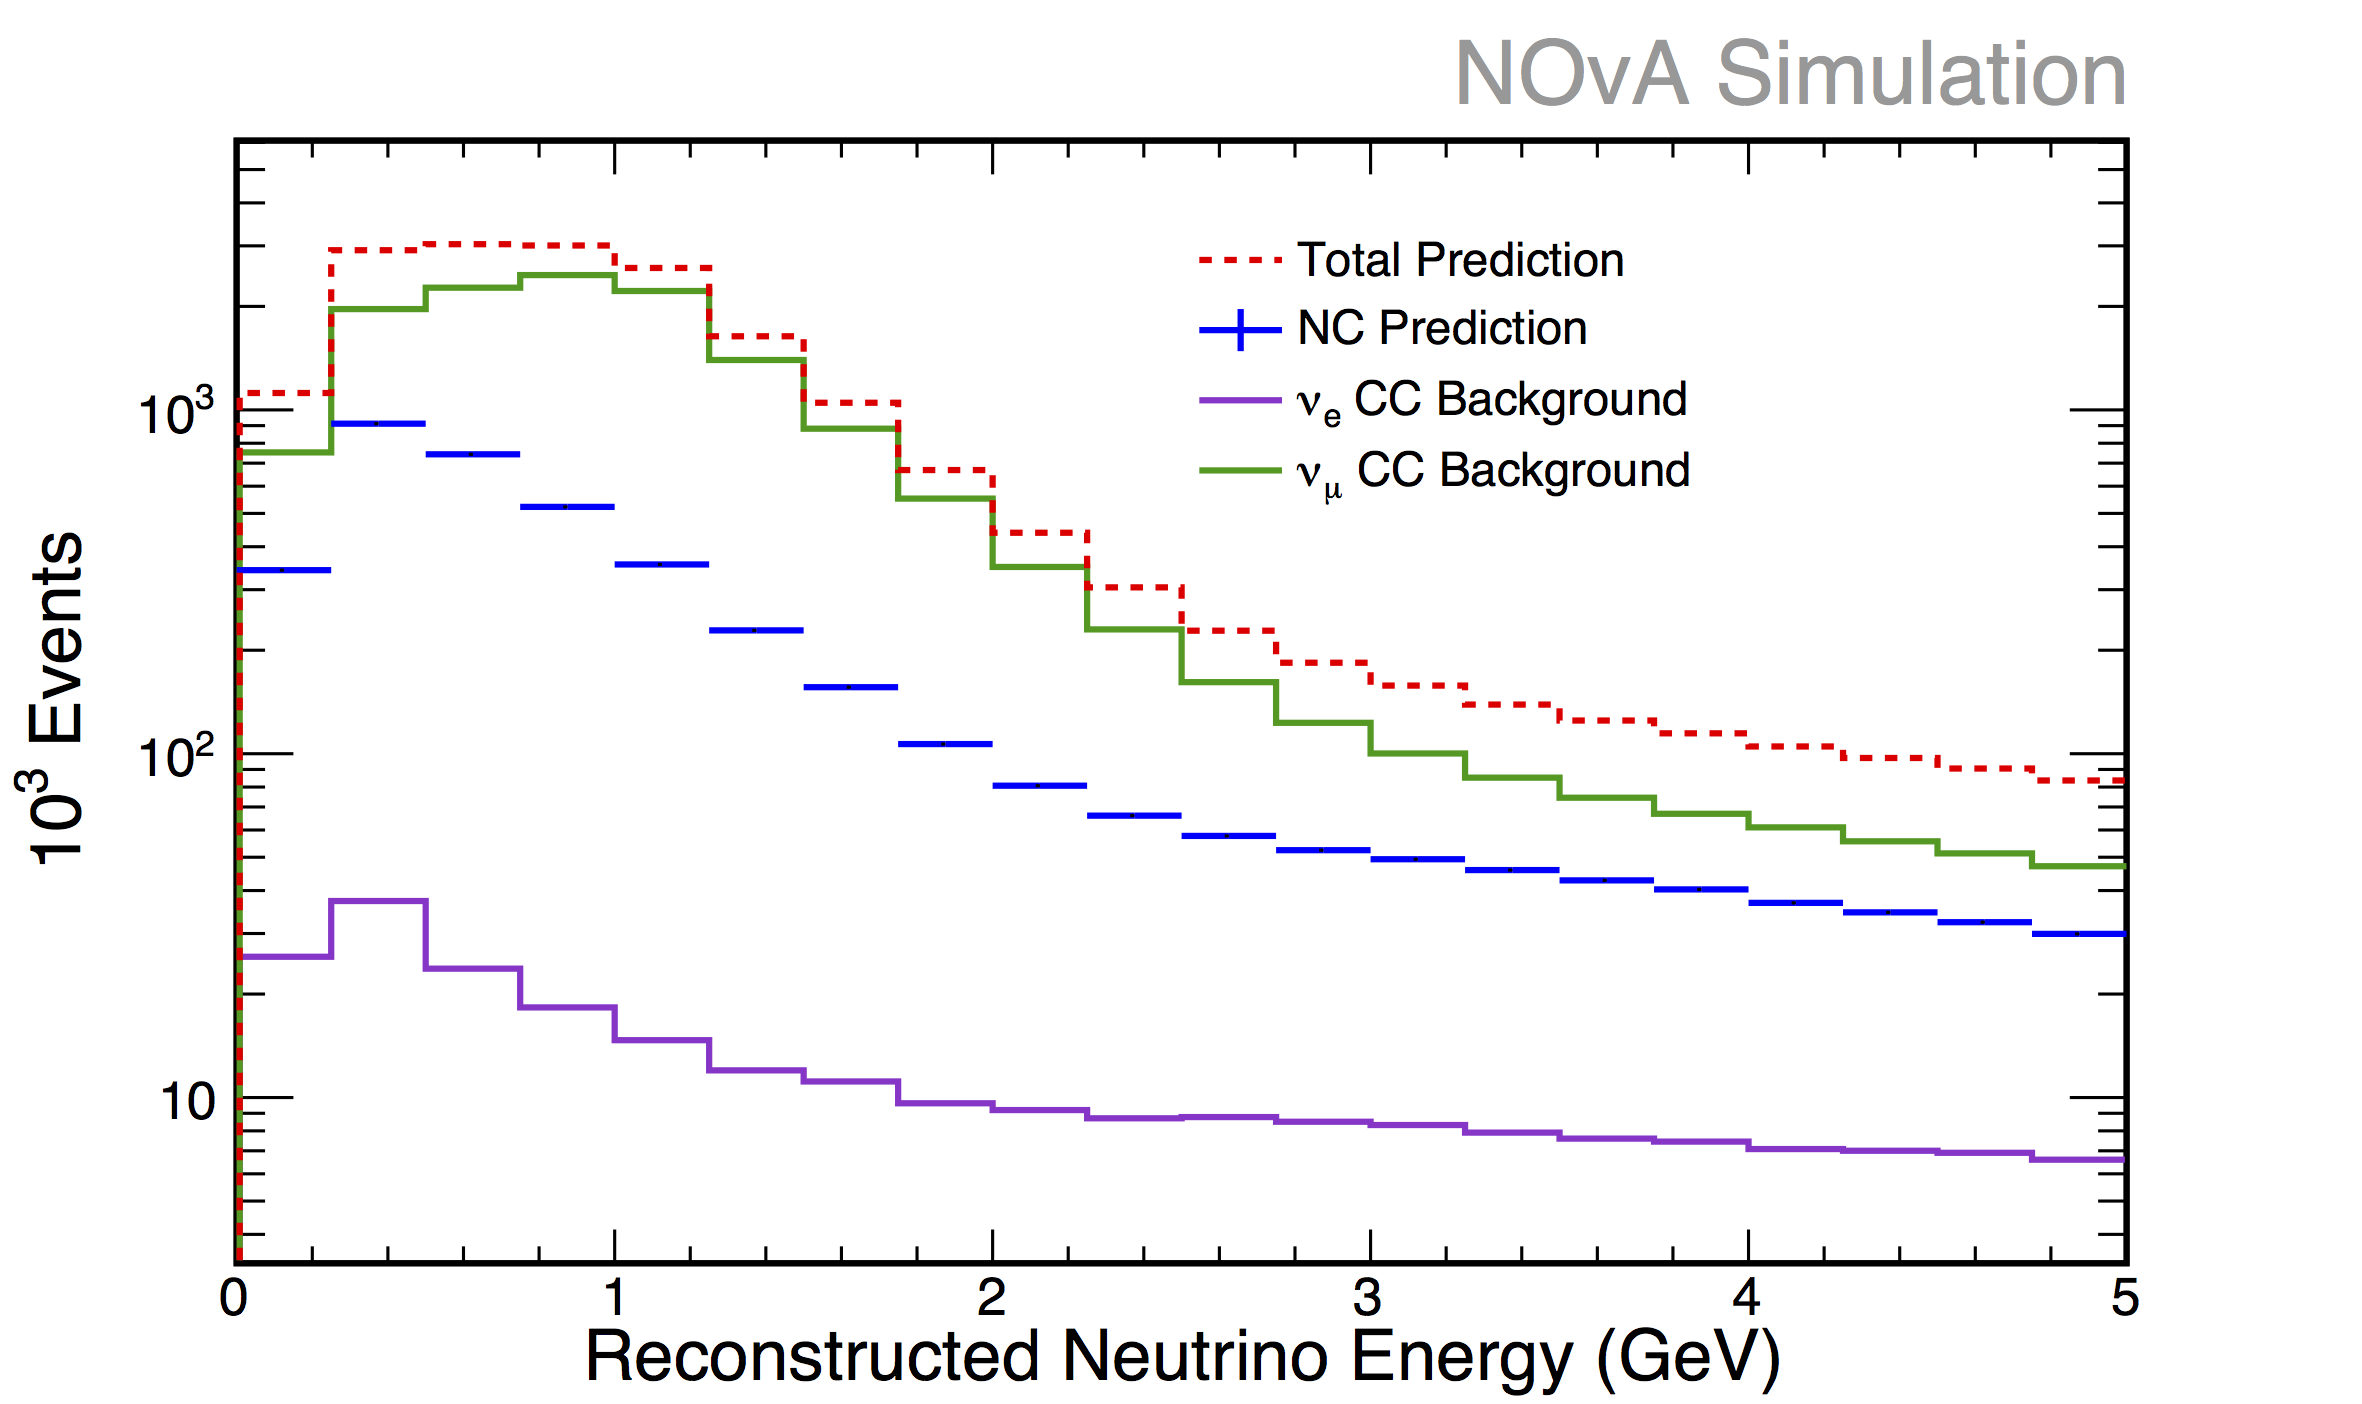
\includegraphics[width=1\linewidth]{figures/RecoE0ND.png}
  \end{subfigure}
  \caption[Energy Spectra After Data Quality Cuts]{Energy spectra after Data Quality cuts for the FD (left) and ND (right).}
  \label{fig:NP1DataQual}
\end{figure}

\section{Event Quality}

Event quality cuts are the first applied to individual events and ensure that there is enough reconstructed information to be properly analyzed and that there were no obvious reconstruction failures. As with the data quality cuts above, these cuts were taken directly from the $\nue$ \cite{ref:EQNuEND, ref:EQNuEFD} and $\numu$ \cite{ref:EQNuMu} analyses. Two of the cuts within this suite simply require the presence of a reconstructed vertex and a shower object. These reconstructed objects are used more extensively in later stages, so the event quality cuts make sure they are available. Other quantities considered are the number of hits per plane, distance between the reconstructed vertex and leading shower, and number of contiguous planes. Events with a high number of hits per plane are cut to remove so called `FEB Flashers,' an event most often triggered by high energy cosmic rays. The events have a signature where all of the cells read out by an FEB appear to be triggered. Events with a low number of contiguous planes are most often associated with very vertical cosmic rays, so events with a low number of planes are cut. Finally, a large distance between a vertex and leading shower is considered a reconstruction failure. These cuts are summarized with the exact parameters used for the cuts in Table \ref{tab:EventQual}. The number of events before and after the event quality cuts are listed in Table \ref{tab:NP1EventQual}, and fig.~\ref{fig:NP1EventQual} shows the energy spectra of the events that pass these cuts.
\begin{table}[h]
  \begin{center}
    \caption[Event Quality Cuts]{Quality cuts applied to individual events to ensure properly reconstructed quantities.}
    \label{tab:EventQual}
    \begin{tabular}{c c c}
      \hline\hline
      Event Quality Metric & Metric for Event to Pass \\
      \hline
      Number of vertex objects & $> 0$ \\
      Number of shower objects & $> 0$ \\
      Number of hits per plane & $< 8$ \\
      Number of contiguous planes & $> 2$ \\
      Distance between vertex and leading shower & $< 100\unit{cm}$ \\
      \hline
    \end{tabular}
  \end{center}
\end{table}

\begin{table}[h]
  \begin{center}
    \caption[Event Table: Event Quality Cuts]{The number of events before and after application of event quality cuts, at both detectors.}
    \label{tab:NP1EventQual}
    \begin{tabular}{c c c c c}
      \hline\hline
      Cut Level & NC & $\numu$ CC & $\nue$ CC & Cosmic \\
      \hline
      \multicolumn{5}{l}{FD:} \\
      Data Quality & 194.8 & 107.3 & 54.0 & 66148.4 \\
      $+$Event Quality & 194.8 & 107.3 & 54.0 & 66148.4 \\
      \multicolumn{5}{l}{ND $(\times 10^{3})$:} \\
      Data Quality & 3934 & 13904 & 246 & \\
      $+$Event Quality & 3934 & 13904 & 246 & \\
      \hline
    \end{tabular}
  \end{center}
\end{table}

\begin{figure}[h]
  \centering
  \begin{subfigure}{.48\textwidth}
    \centering
    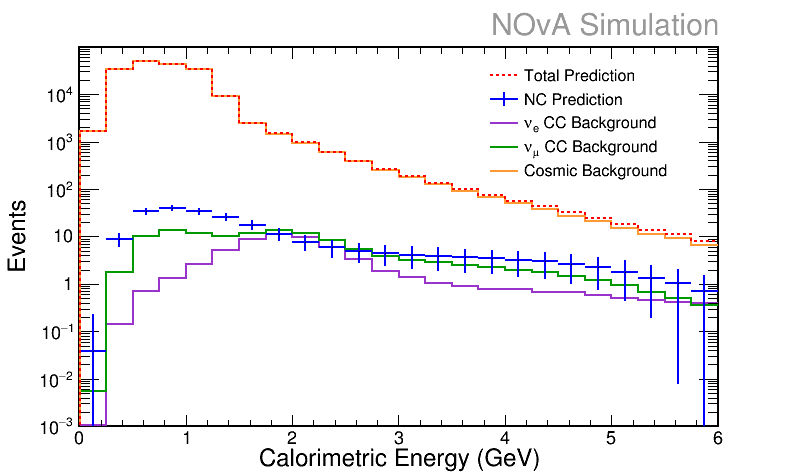
\includegraphics[width=1\linewidth]{figures/RecoE1FD.png}
  \end{subfigure}
  \begin{subfigure}{.48\textwidth}
    \centering
    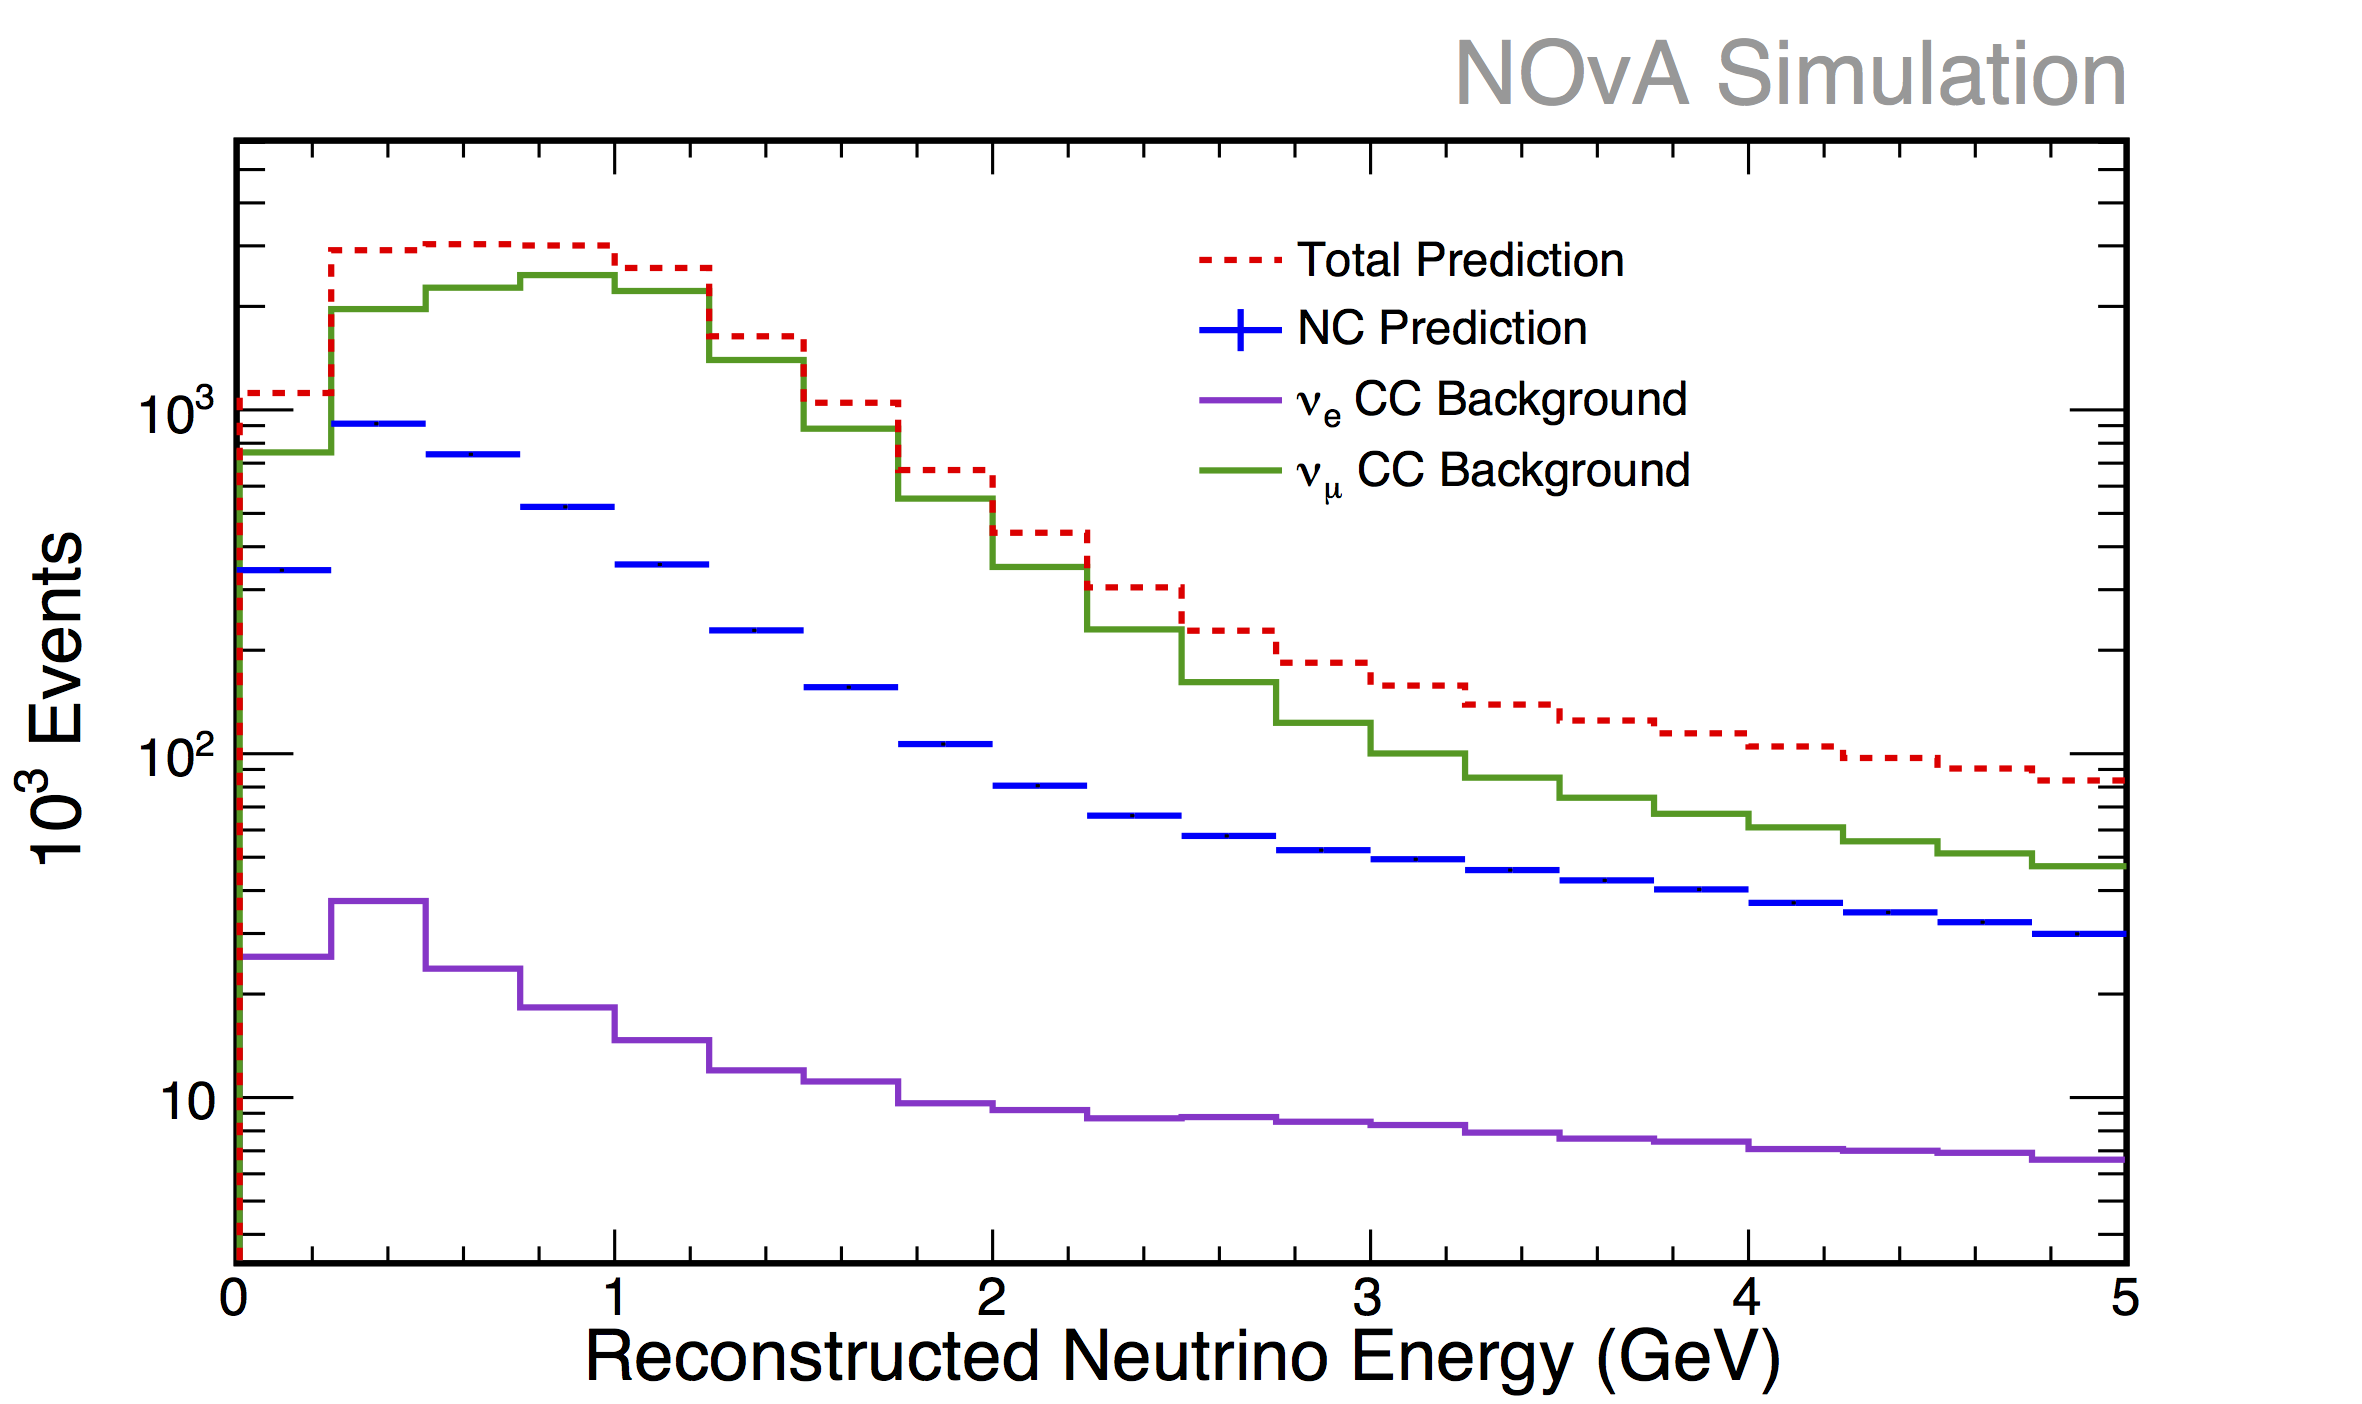
\includegraphics[width=1\linewidth]{figures/RecoE1ND.png}
  \end{subfigure}
  \caption[Energy Spectra After Event Quality Cuts]{Energy spectra after Event Quality cuts for the FD (left) and ND (right).}
  \label{fig:NP1EventQual}
\end{figure}

\section{Fiducial Volume and Containment}

Fiducial volume and containment cuts are applied to remove events originating outside of the detector and to ensure that events originating inside of the detector do not have activity that escapes the detector. The fiducial volume cut is a cut on the location of the reconstructed neutrino vertex. The containment cut considers the leading shower of an event and cuts the event if the start or stop point is too close to a detector wall. The specific cuts were set separately at each detector.

\subsection{Far Detector}

For the FD, the fiducial and containment cuts are the first major step in reducing the cosmic background. Since cosmic ray events originate above the detector, there are many more cosmic events with reconstructed vertices in the upper portion of the detector. The fiducial volume cut in $Y$ is thus applied in an asymmetric way to eliminate more of the cosmic background. The fiducial volume cut on $Z$ (the beam direction) is also asymmetric to account for cosmic rays entering the back of the detector hall where there is a smaller amount of rock overburden to shield these events. The fiducial volume cut on $X$ is also applied slightly asymmetrically for a slight performance gain. Events that pass these fiducial cuts must still pass the containment cuts. For the FD, the start and stop points of the leading prong must be further than $10\unit{cm}$ of any detector face. Fig.~\ref{fig:FidCont} shows the distributions of these variables before application of the fiducial or containment cuts. Table \ref{tab:NP1FidContFD} summarizes the event rates before and after applying fiducial and containment cuts; fig.~\ref{fig:NP1FidContFD} show the energy spectra of events that pass these cuts.
\begin{figure}[h]
  \centering
  \begin{tabular}{c c}
    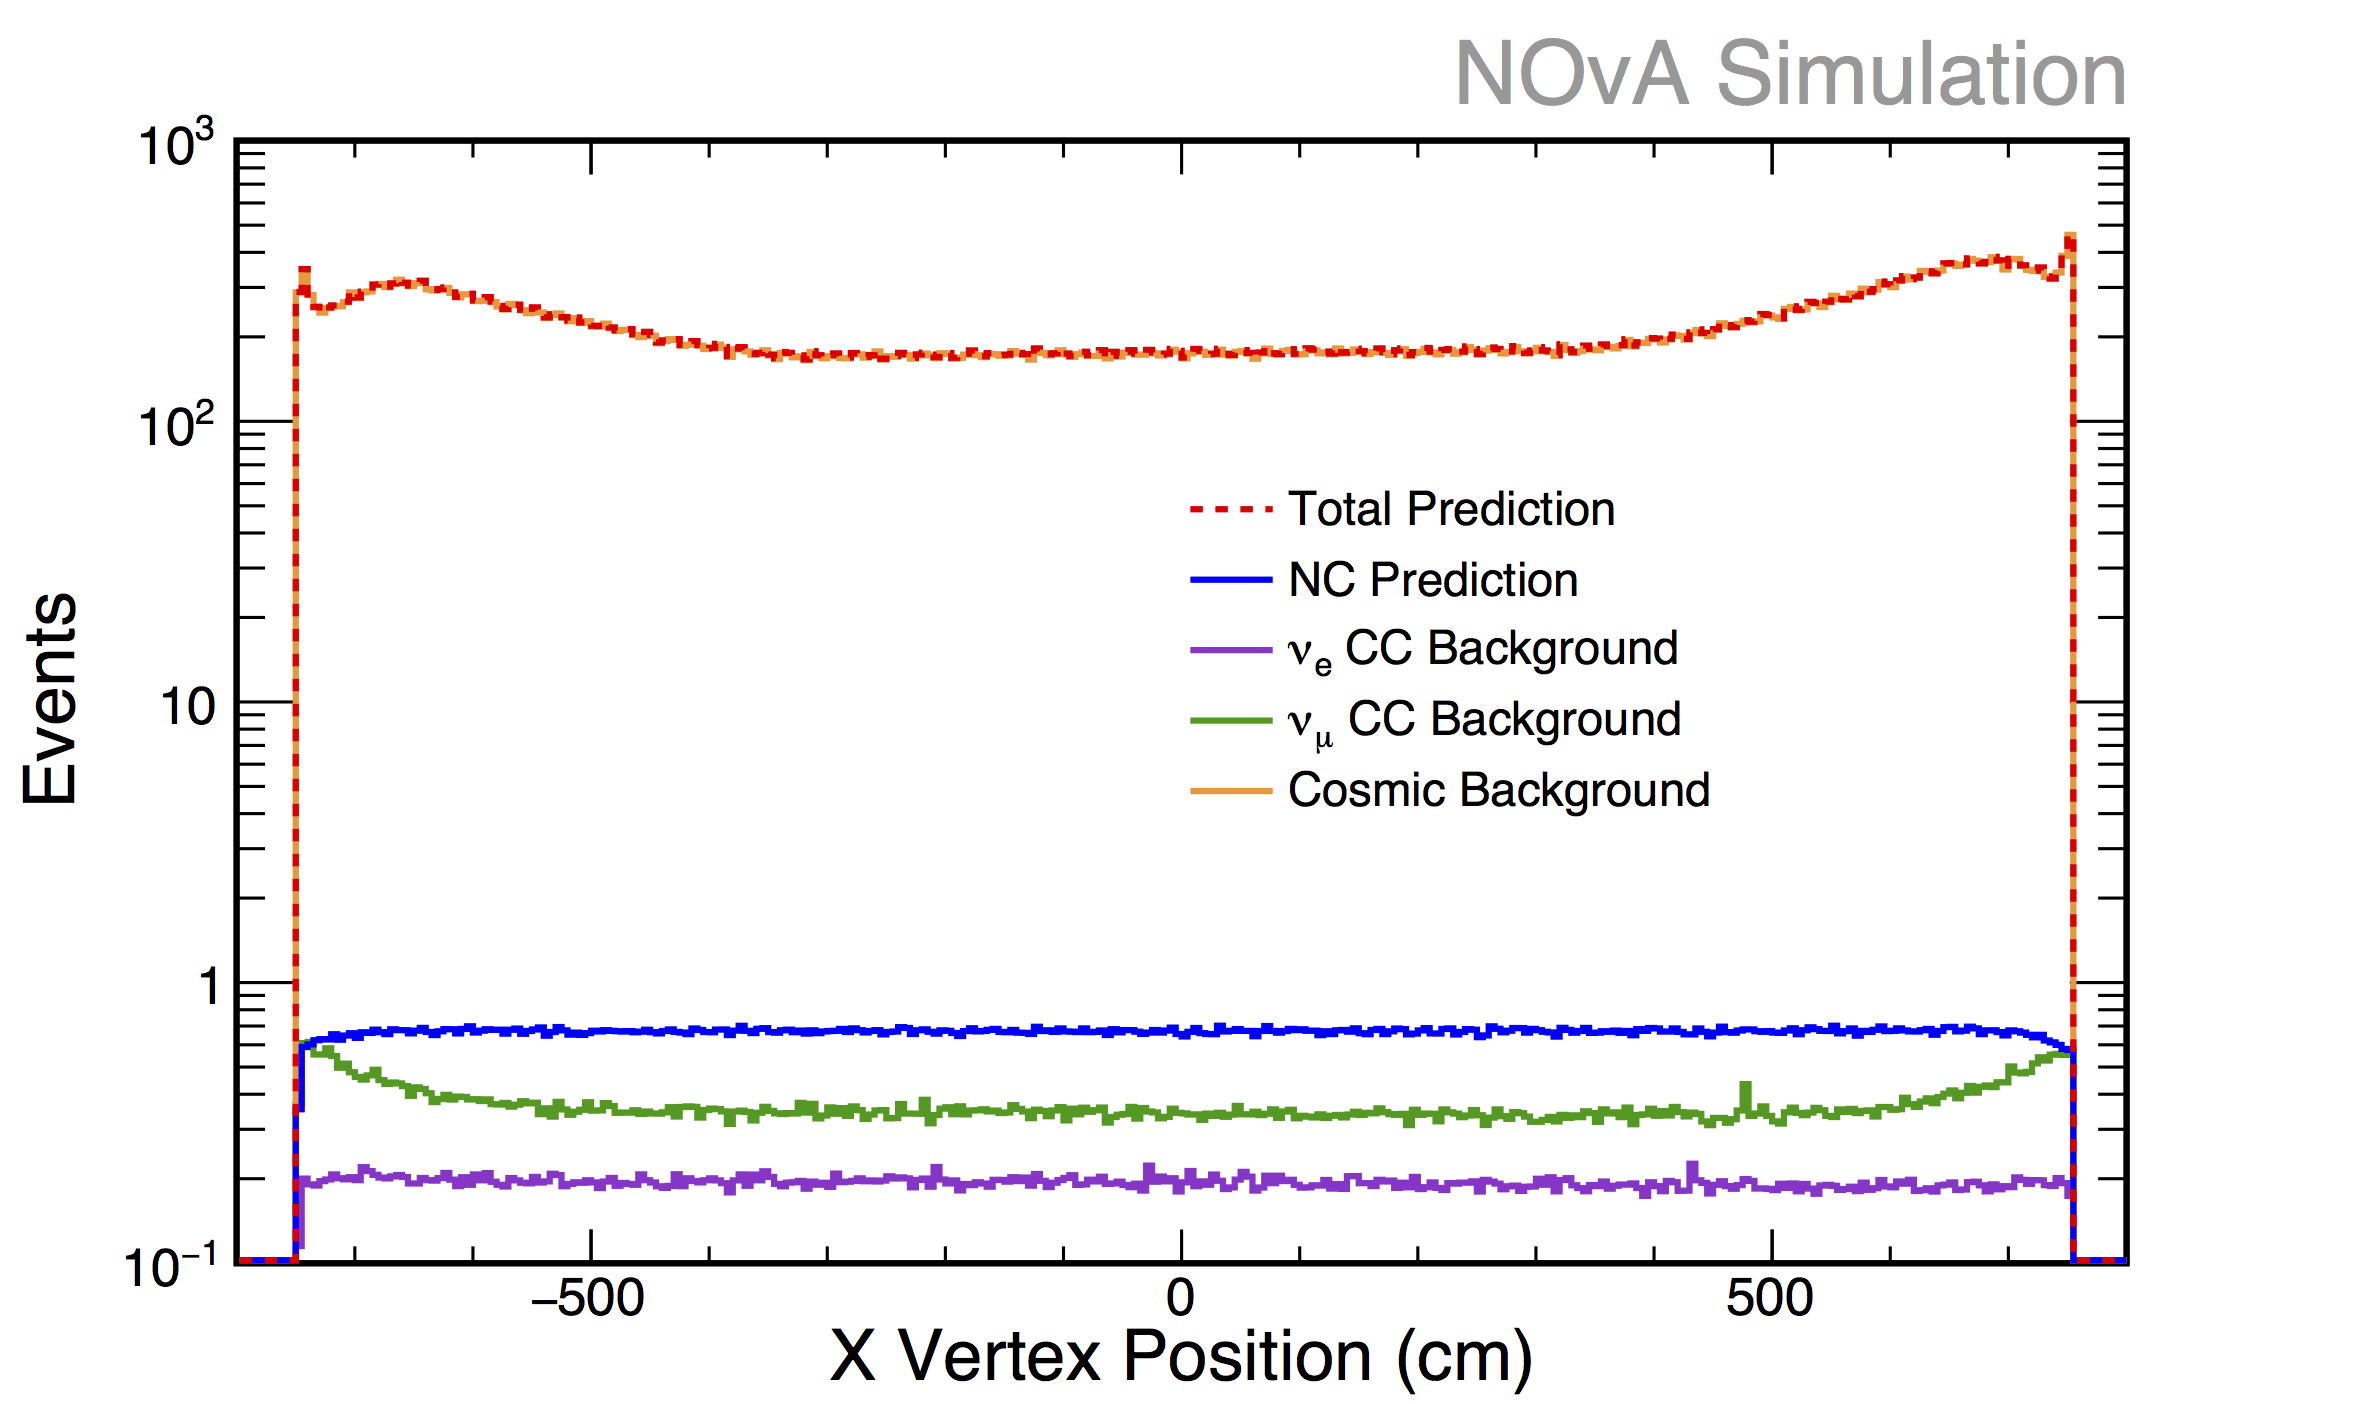
\includegraphics[width=.48\textwidth]{figures/NP1VtxX.png} &
    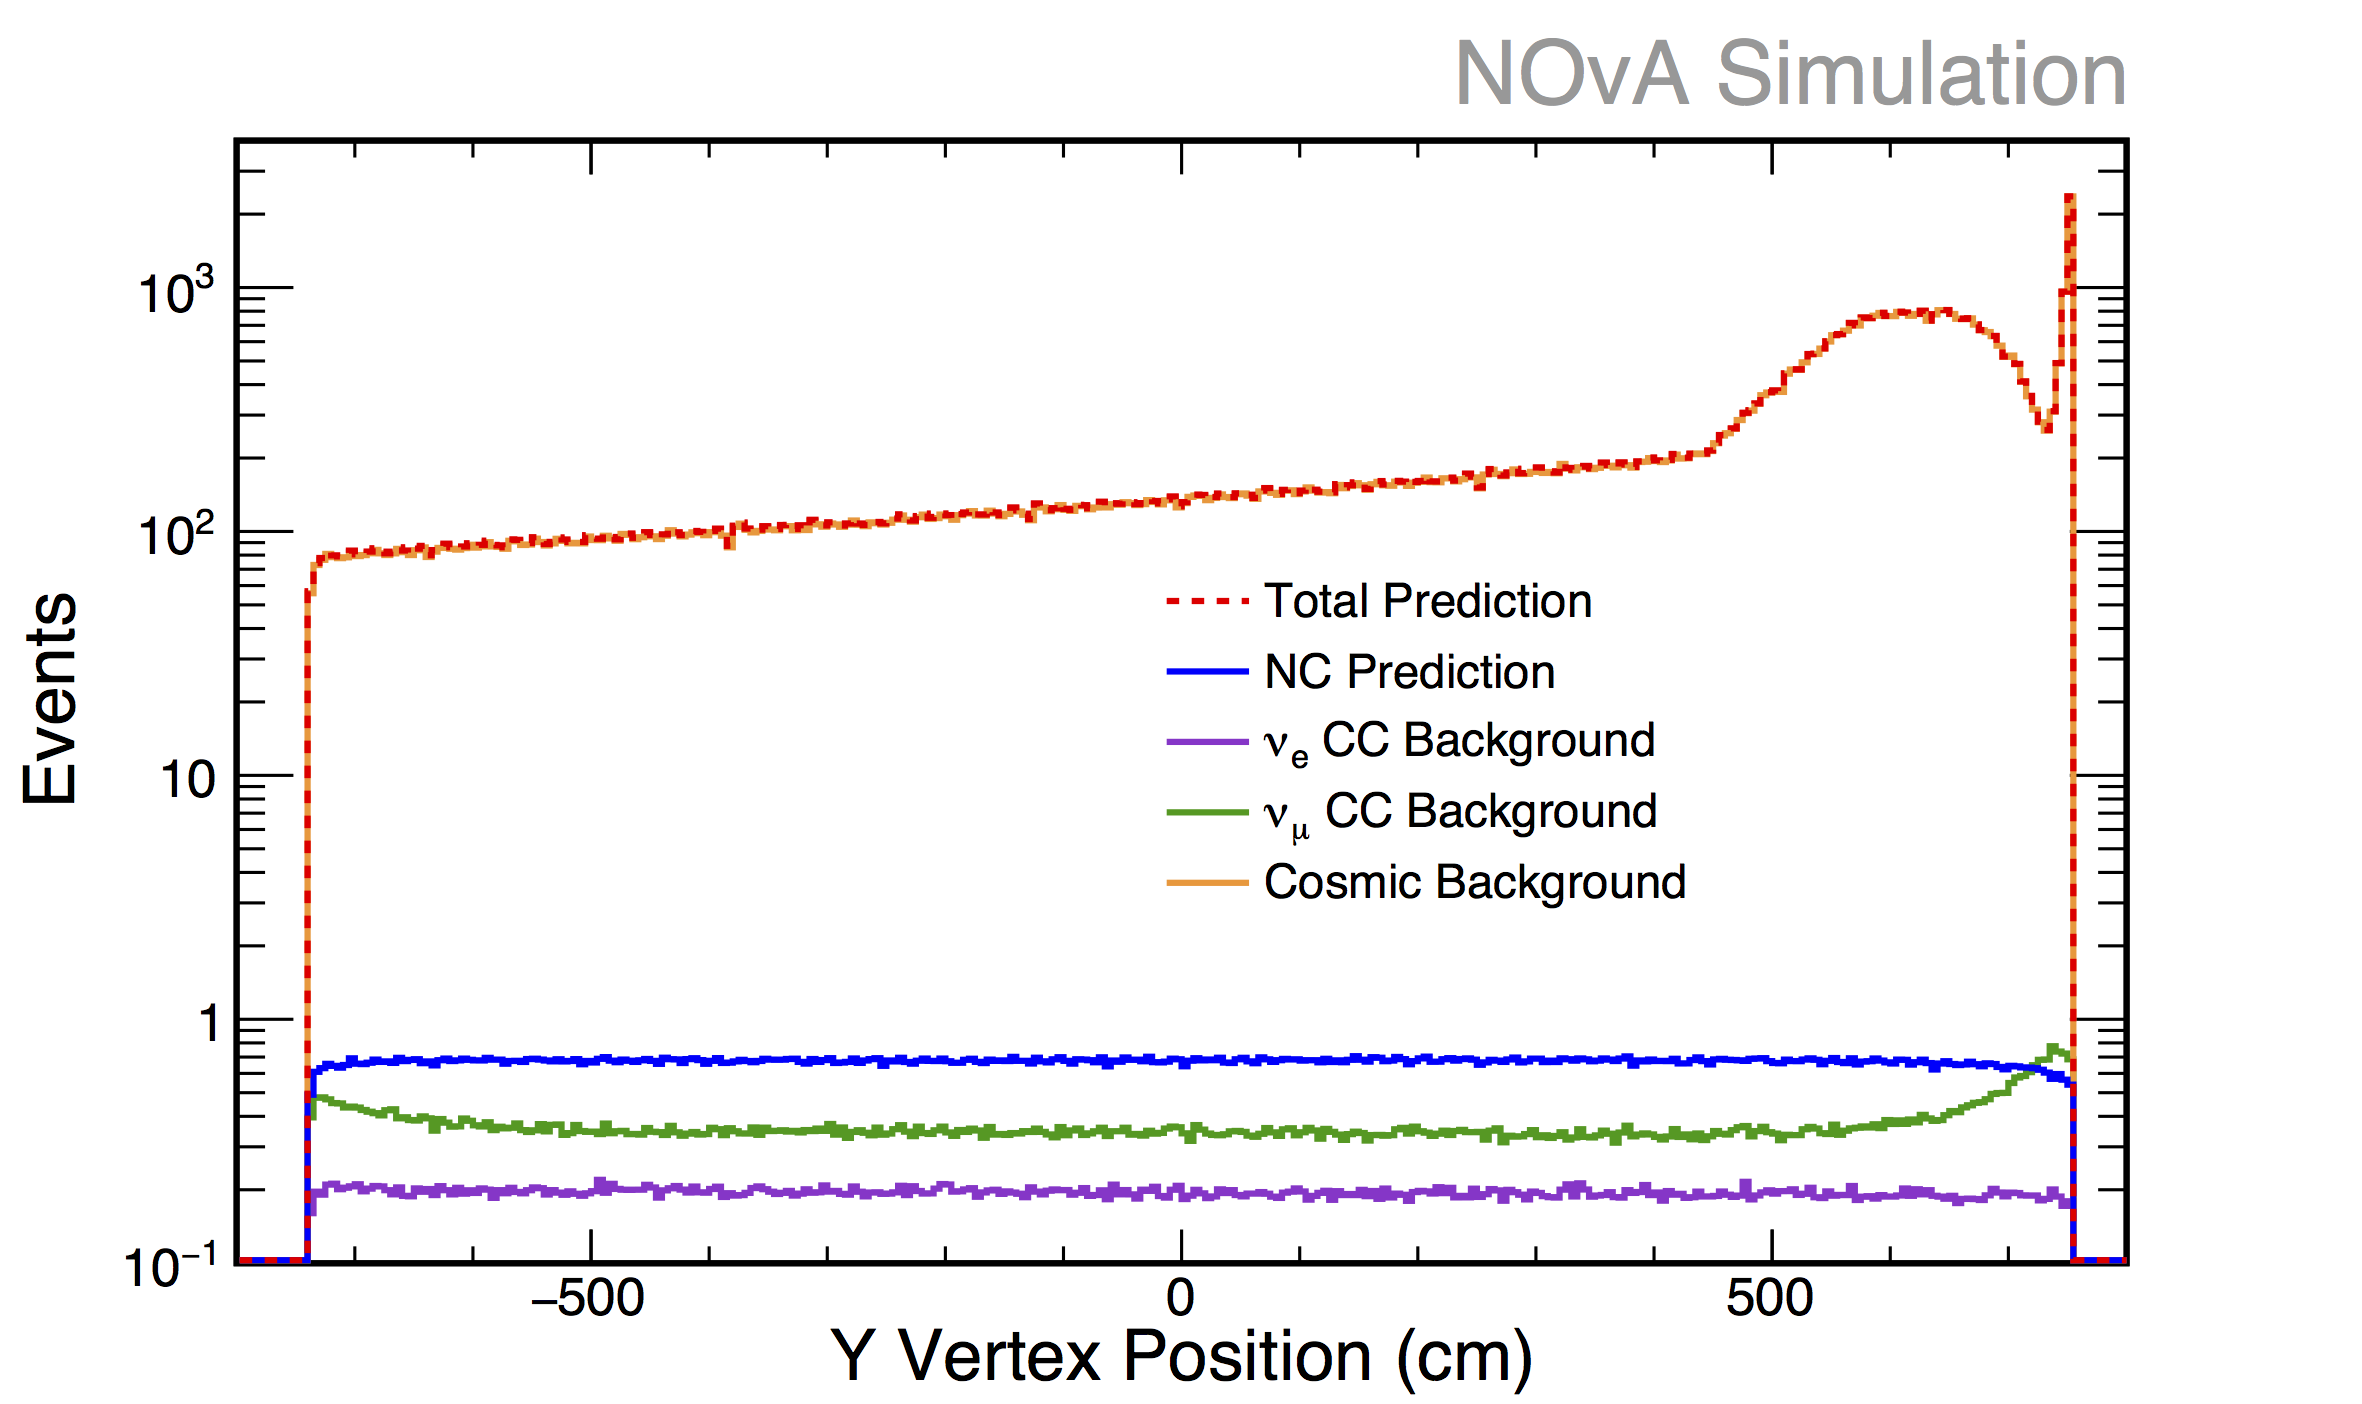
\includegraphics[width=.48\textwidth]{figures/NP1VtxY.png} \\
    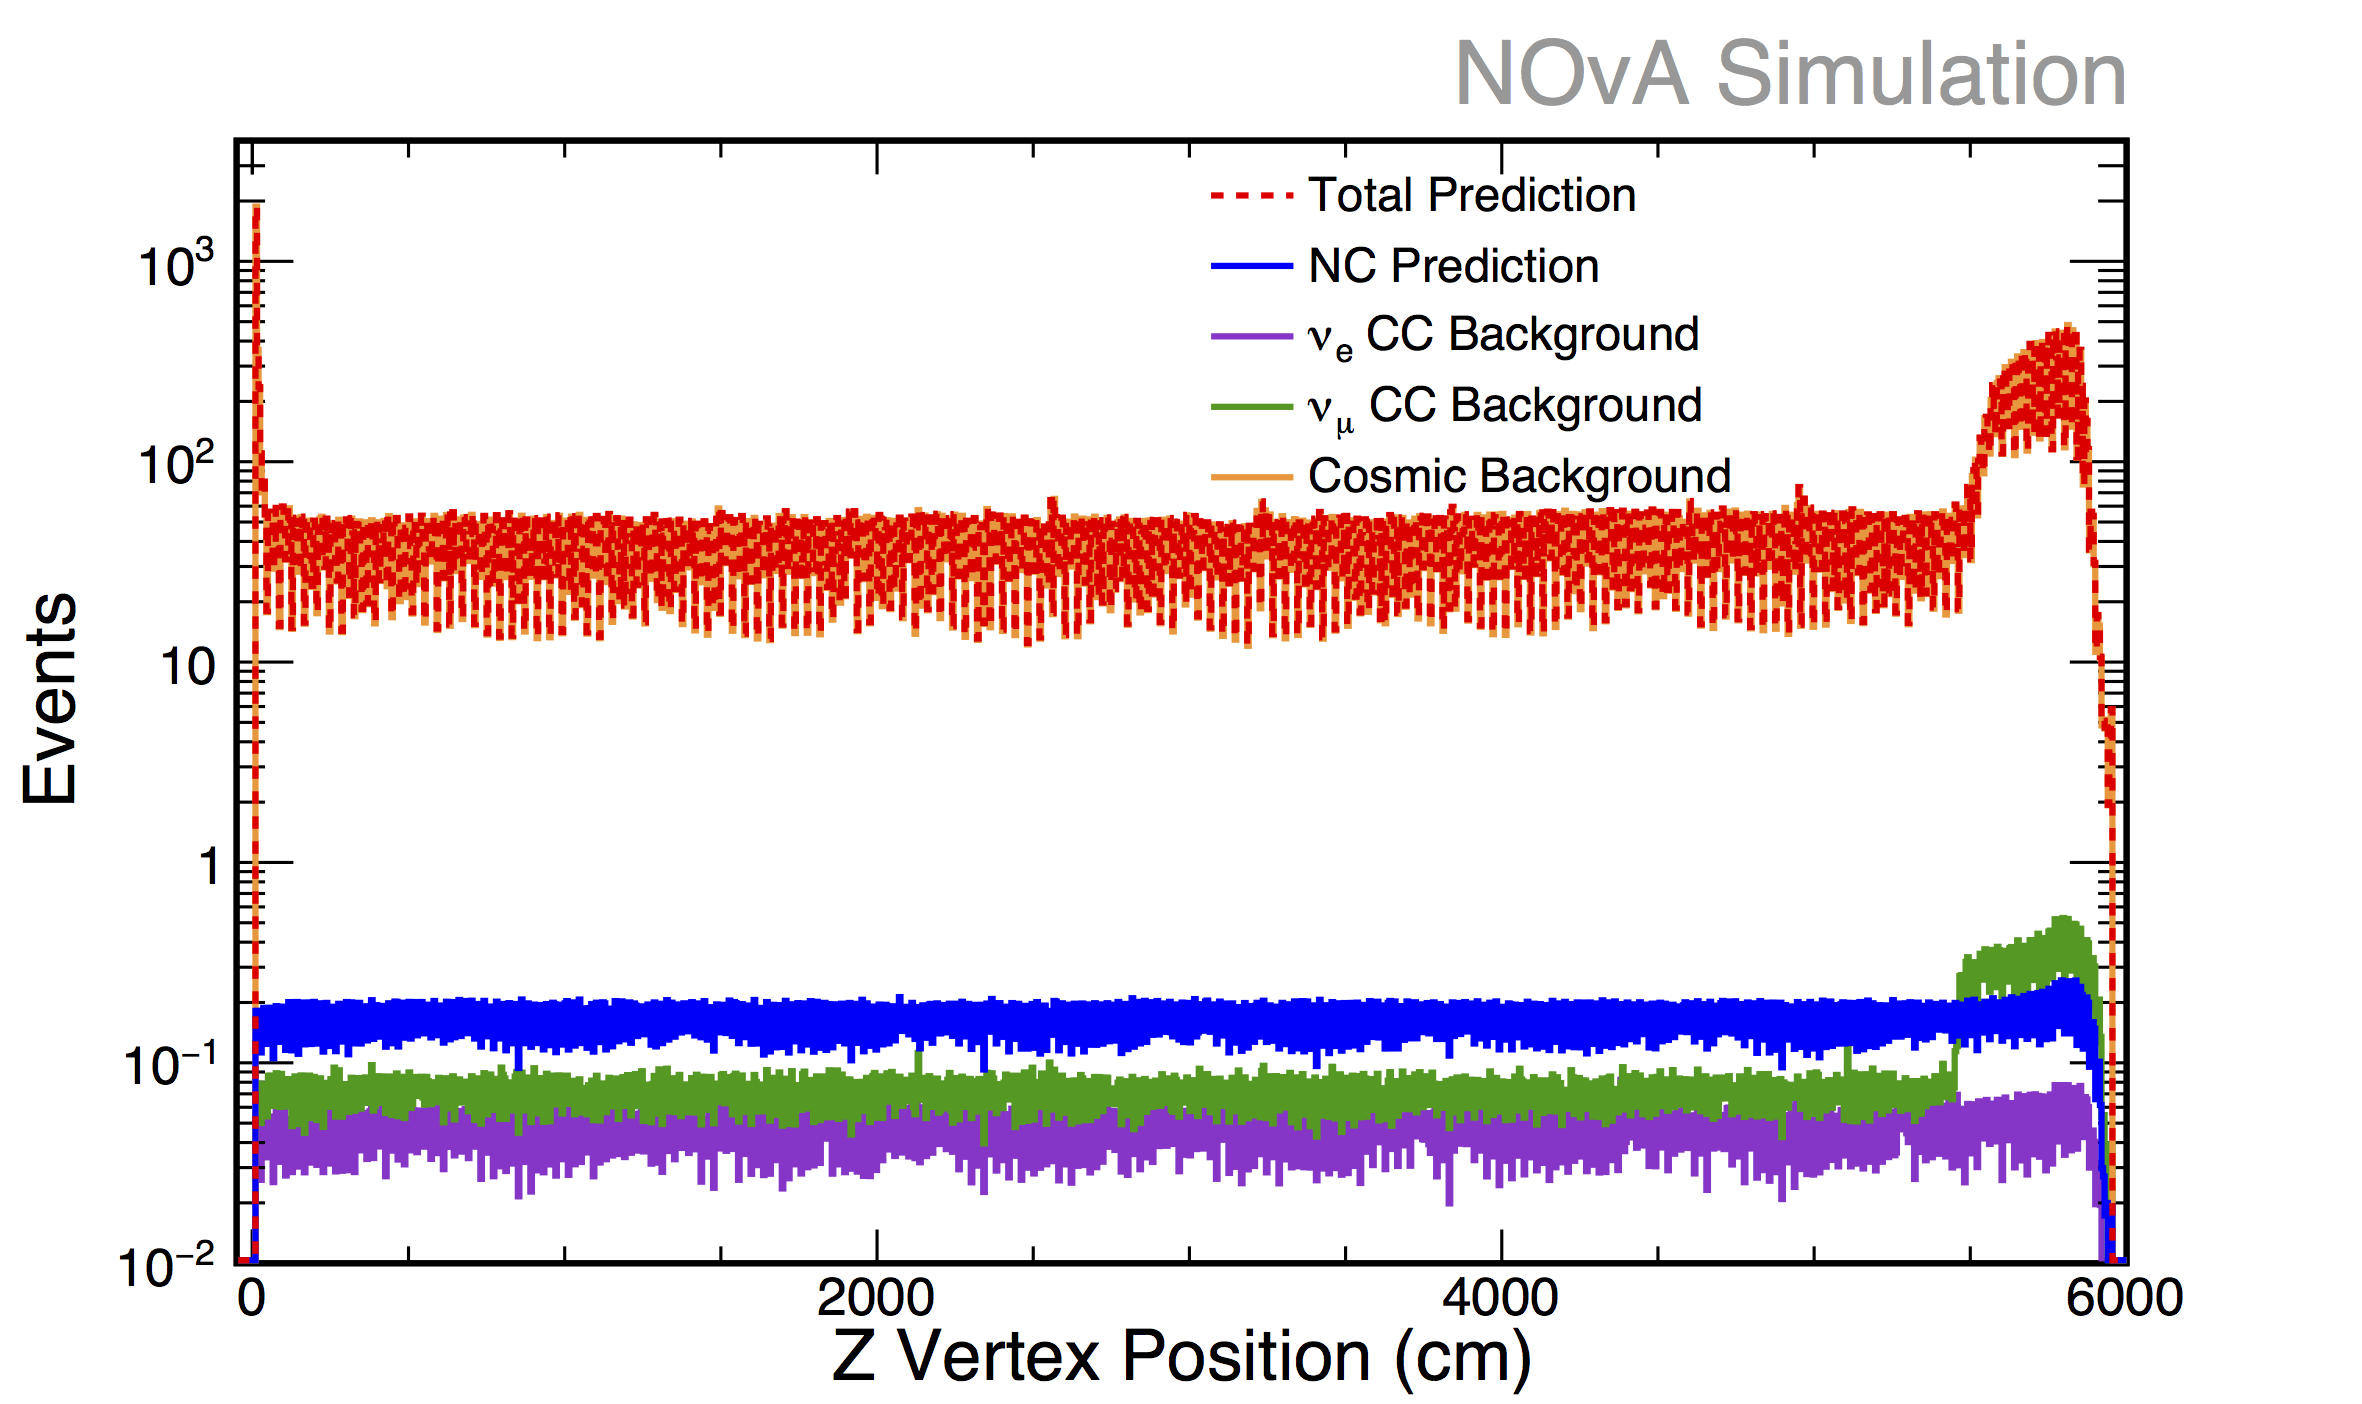
\includegraphics[width=.48\textwidth]{figures/NP1VtxZ.png} &
    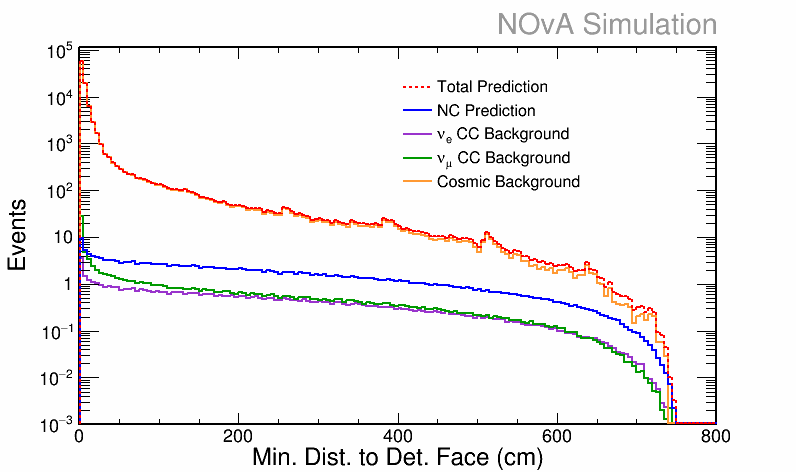
\includegraphics[width=.48\textwidth]{figures/NP1Cont.png} \\
  \end{tabular}
  \caption[Fiducial and Containment Variable Distributions]{Distributions of variables used for fiducial and containment cuts at the FD. The top left, top right, and bottom left show the distributions of the reconstructed vertex. The bottom right shows the minimum distance between the start or stop of the leading prong to any detector face.}
  \label{fig:FidCont}
\end{figure}

\begin{table}[h]
  \begin{center}
    \caption[FD Fiducial and Containment Cuts]{Fiducial and containment cuts applied to events in the FD.}
    \label{tab:FidContFD}
    \begin{tabular}{c c c}
      \hline\hline
      Reconstructed Quantity & Metric for Event to Pass \\
      \hline
      Reconstructed Vertex X Coordinate & $-680\unit{cm} \leq vtxX \leq 650\unit{cm} $ \\
      Reconstructed Vertex Y Coordinate & $-720\unit{cm} \leq vtxY \leq 600\unit{cm}$ \\
      Reconstructed Vertex Z Coordinate & $50\unit{cm} \leq vtxZ \leq 5450\unit{cm}$ \\
      Leading prong start/stop distance to detector face & $> 10\unit{cm}$ \\
      \hline
    \end{tabular}
  \end{center}
\end{table}

\begin{table}[h]
  \begin{center}
    \caption[Event Table: Fiducial and Containment Cuts, FD]{The number of events before and after application of fiducial and containment cuts at the FD.}
    \label{tab:NP1FidContFD}
    \begin{tabular}{c c c c c}
      \hline\hline
      Cut Level & NC & $\numu$ CC & $\nue$ CC & Cosmic \\
      \hline
      ...Event Quality & 194.8 & 107.3 & 54.0 & 66148.4 \\
      $+$ Fiducial & 116.7 & 45.5 & 32.2 & 8164.7 \\
      $+$ Containment & 113.2 & 39.7 & 31.0 & 580.0 \\
      \hline
    \end{tabular}
  \end{center}
\end{table}

\begin{figure}[h]
  \centering
  \begin{subfigure}{.48\textwidth}
    \centering
    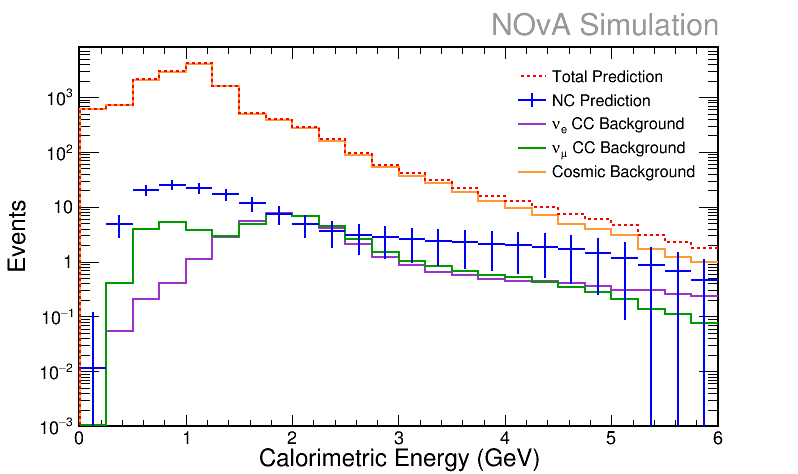
\includegraphics[width=1\linewidth]{figures/RecoE2FD.png}
  \end{subfigure}
  \begin{subfigure}{.48\textwidth}
    \centering
    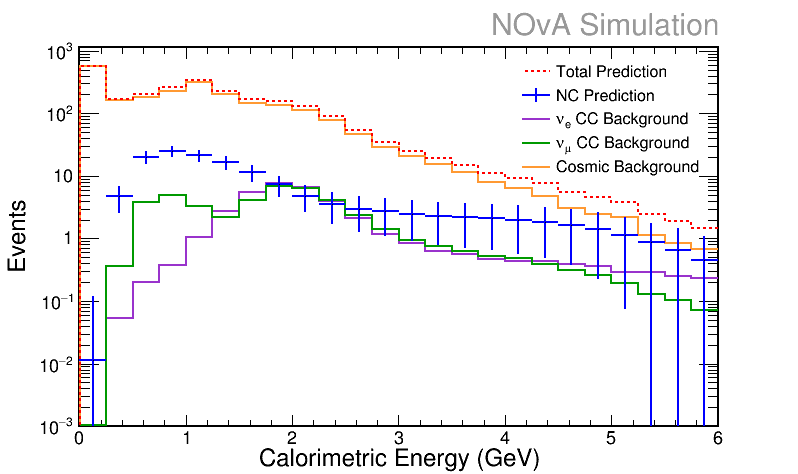
\includegraphics[width=1\linewidth]{figures/RecoE3FD.png}
  \end{subfigure}
  \caption[Energy Spectra After Fiducial and Containment Cuts, FD]{Energy spectra after fiducial and containment cuts for the FD. On the left, the cuts applied are data quality, event quality, and fiducial. The right plot also includes the containment cut.}
  \label{fig:NP1FidContFD}
\end{figure}

\subsection{Near Detector}

While the ND does not have a large cosmic background to eliminate, there are many events that originate in the rock outside of the detector that can leak into the detector. Furthermore, the small size of the ND means that many events have activity that escapes outside of the detector. The fiducial and containment cuts at the ND are designed to combat both of these effects. The fiducial cuts on the $X$ and $Y$ coordinates of the reconstructed vertex were applied symmetrically, with a modestly large cut to remove events that originate in the rock outside the detector. The vertex cut on $Z$ also cuts a large portion of the detector to cut rock events that leak into the front of the detector. The containment cuts at the ND are more strict than the FD. The leading prong is required to be greater than $25\unit{cm}$ from each detector face, and every track in the event is also subject to this cut. For the cut on each track, the back `face' of the detector is considered to be the last plane of the fully active portion of the detector, effectively cutting events with activity in the muon catcher. All of these cuts are summarized in Table \ref{tab:FidContND}, Table \ref{tab:NP1FidContND} lists the event rates before and after the cuts are applied, and fig.~\ref{fig:NP1FidContND} shows the energy spectra of events that pass these cuts.
\begin{table}[h]
  \begin{center}
    \caption[ND Fiducial and Containment Cuts]{Fiducial and containment cuts applied to events in the ND.}
    \label{tab:FidContND}
    \begin{tabular}{c c c}
      \hline\hline
      Reconstructed Quantity & Metric for Event to Pass \\
      \hline
      Reconstructed Vertex X Coordinate & $-100\unit{cm} \leq vtxX \leq 100\unit{cm} $ \\
      Reconstructed Vertex Y Coordinate & $-100\unit{cm} \leq vtxY \leq 100\unit{cm}$ \\
      Reconstructed Vertex Z Coordinate & $200\unit{cm} \leq vtxZ \leq 1000\unit{cm}$ \\
      Leading prong start/stop point, distance to detector face & $> 25\unit{cm}$ \\
      Each track start/stop point, distance to detector face & $> 25\unit{cm}$ \\
      \hline
    \end{tabular}
  \end{center}
\end{table}

\begin{table}[h]
  \begin{center}
    \caption[Event Table: Fiducial and Containment Cuts, ND]{The number of events before and after application of fiducial and containment cuts at the ND. Here, containment refers to cuts on the distance of the leading prong and each track to the closest detector face.}
    \label{tab:NP1FidContND}
    \begin{tabular}{c c c c}
      \hline\hline
      Cut Level & NC & $\numu$ CC & $\nue$ CC \\
      \hline
      ...Event Quality & 3934 & 13904 & 246 \\
      $+$ Fiducial & 1377 & 3490 & 64 \\
      $+$ Containment & 686.0 & 809.7 & 26.8 \\
      \hline
    \end{tabular}
  \end{center}
\end{table}

\begin{figure}[h]
  \centering
  \begin{subfigure}{.48\textwidth}
    \centering
    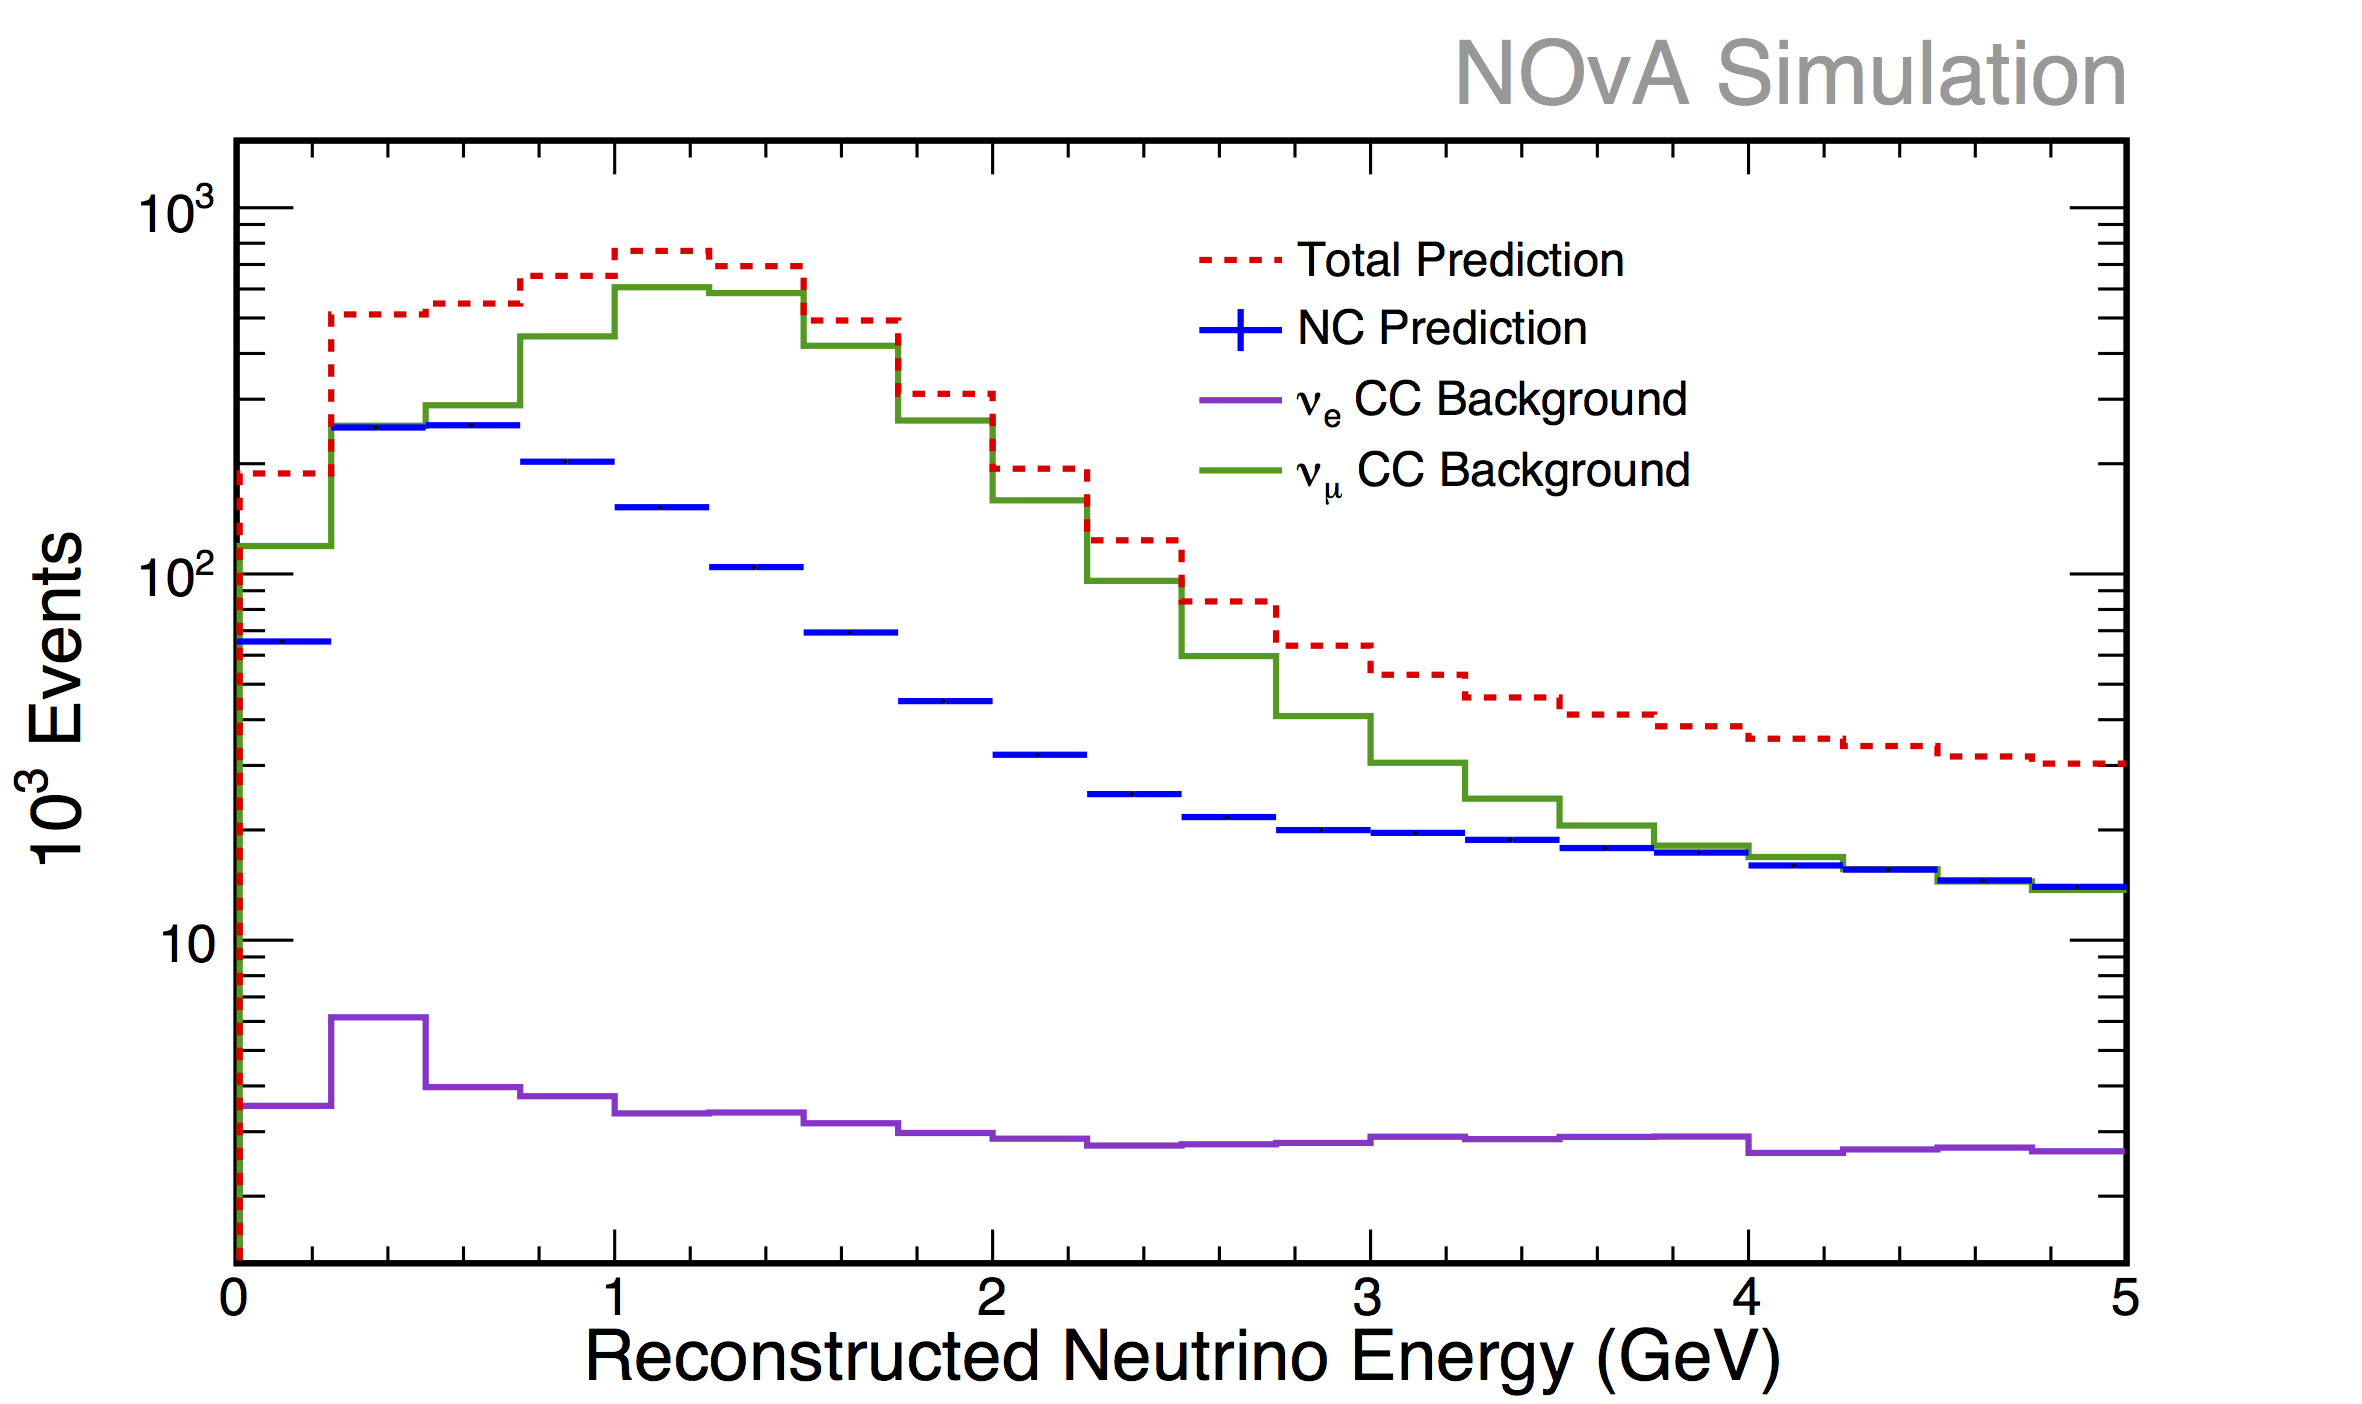
\includegraphics[width=1\linewidth]{figures/RecoE2ND.png}
  \end{subfigure}
  \begin{subfigure}{.48\textwidth}
    \centering
    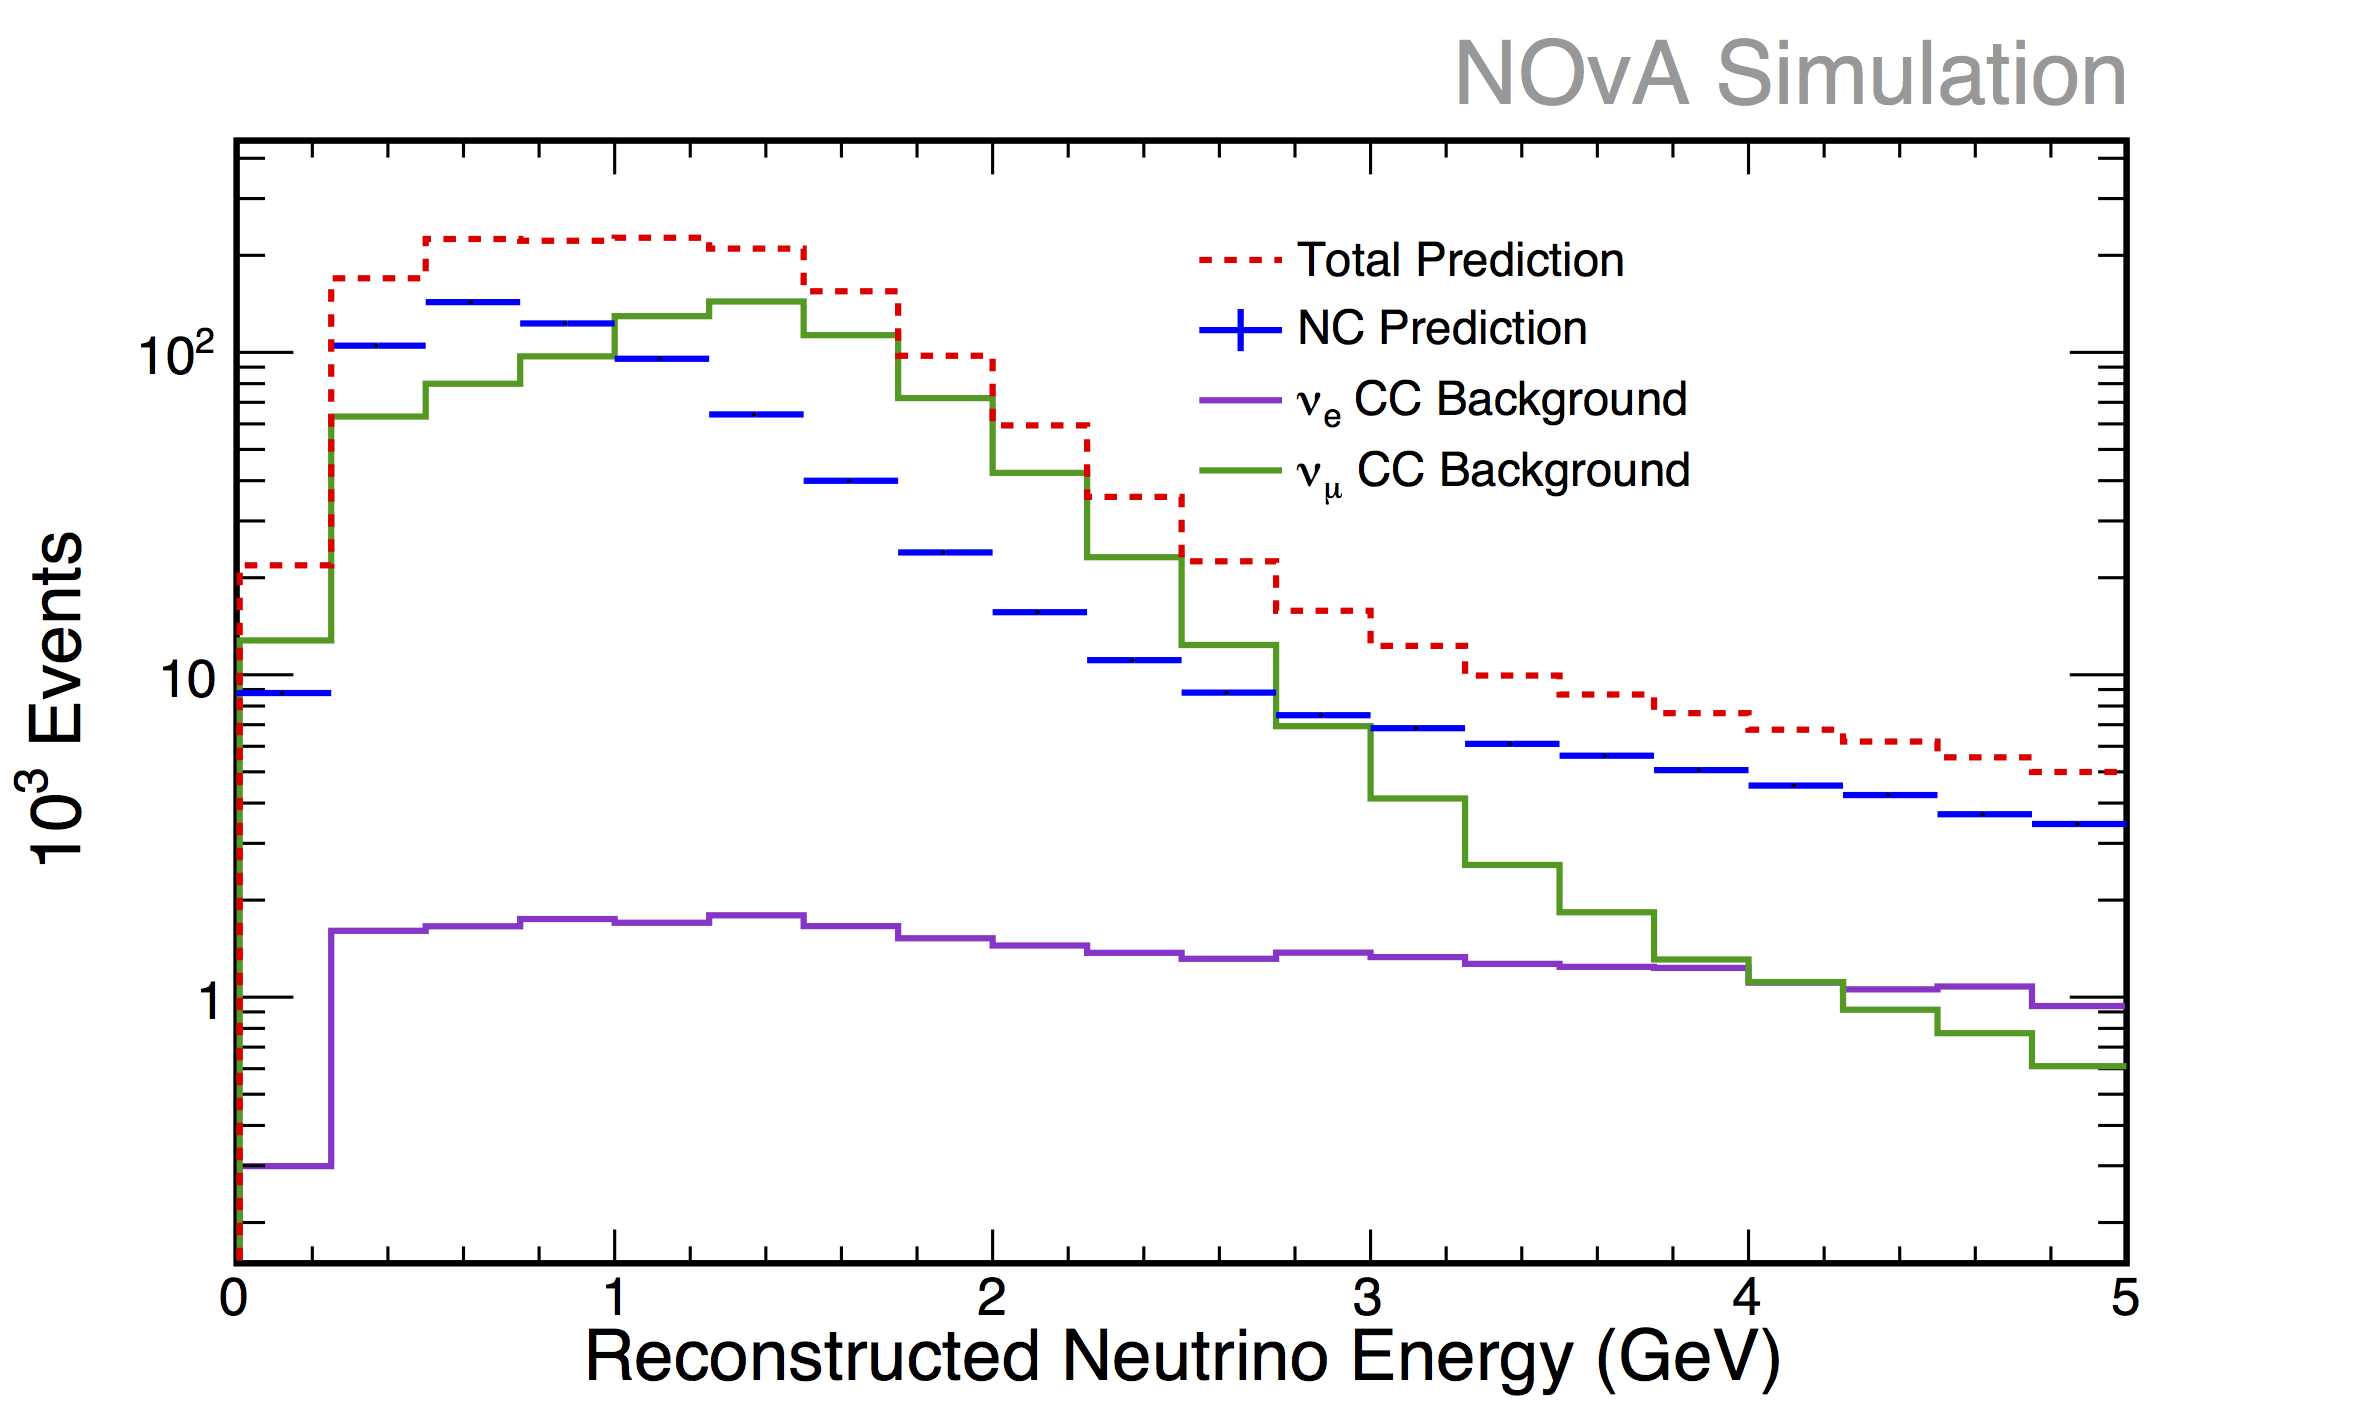
\includegraphics[width=1\linewidth]{figures/RecoE3ND.png}
  \end{subfigure}
  \caption[Energy Spectra After Fiducial and Containment Cuts, ND]{Energy spectra after fiducial and containment cuts for the ND. On the left, the cuts applied are data quality, event quality, and fiducial. The right plot also includes the containment cuts.}
  \label{fig:NP1FidContND}
\end{figure}

\section{NC Selection}

All of the cuts discussed to this point ensure that the remaining sample of events are well reconstructed, contained events. The remaining events should all be representative of their respective types, i.e., NC, $\nue$ CC, and $\numu$ CC. The NC selection cuts are designed to select a relatively pure sample of NC events from amongst the CC backgrounds. The LID, RemID, and CVN PID distributions all have power to complete this goal, though only CVN was ultimately the only PID used. Finally, we use a cut on the number of hits for a small performance gain at the ND.

CVN, discussed in detail in ref.~\cite{ref:TNCVN}, does not attempt to identify a single event type; rather, it gives the most likely event type among all possibilities. CVN is a convolutional neural network that only takes the raw event topology as input. The algorithm applies a series of convolutional filters to search for key event features as opposed to taking these features as input, then trains against these features. Since this PID attempts to classify all event types, cutting events that have a low NC score removes a significant majority of all background types.

RemID, discussed in detail in ref.~\cite{ref:TNRemID}, is specifically designed to identify muons from charged pions, and provides separation power to remove $\numu$ CC events that score highly under this PID. The PID is trained using a $k-$Nearest Neighboor classification on four input variables for a reconstructed track, the track energy deposition log likelihood, a scattering log likelihood, the track length, and the fraction of planes passed by the track that are uncontaminated by vertex or hadronic activity.

LID, described in ref.~\cite{ref:TNLID}, has the power to remove $\nue$ CC events. This PID uses an artificial neural network to test the most energetic shower against electron, muon, proton, neutron, pion (charged and neutral), and photon hypothesis. The main inputs to this PID are the longitudinal and transverse energy deposition, but it also considers the fraction of event energy contained in the primary shower, the invariant mass of all event showers, the energy contained within eight planes of the vertex, the distance between the event vertex and shower start point, and the angle of the shower away from the beam direction.

Chronologically, CVN was developed later than RemID and LID, thus these PIDs were originally used to develop the analysis. While they were replaced by CVN as the sole PID used in the analysis, they nevertheless provided a valuable check that CVN was behaving sensibly. The PID distributions for RemID and LID were studied before and after applying the cut chosen on CVN to ensure that it was removing largely the same events, and if there were any other minor performance increases to be gained. Fig.~\ref{fig:NCSelRemLID} shows these distributions. Based on the results, it was decided that CVN provided all of the necessary separation power and so RemID and LID were not used in the analysis.
\begin{figure}[h]
  \centering
  \begin{tabular}{c c}
    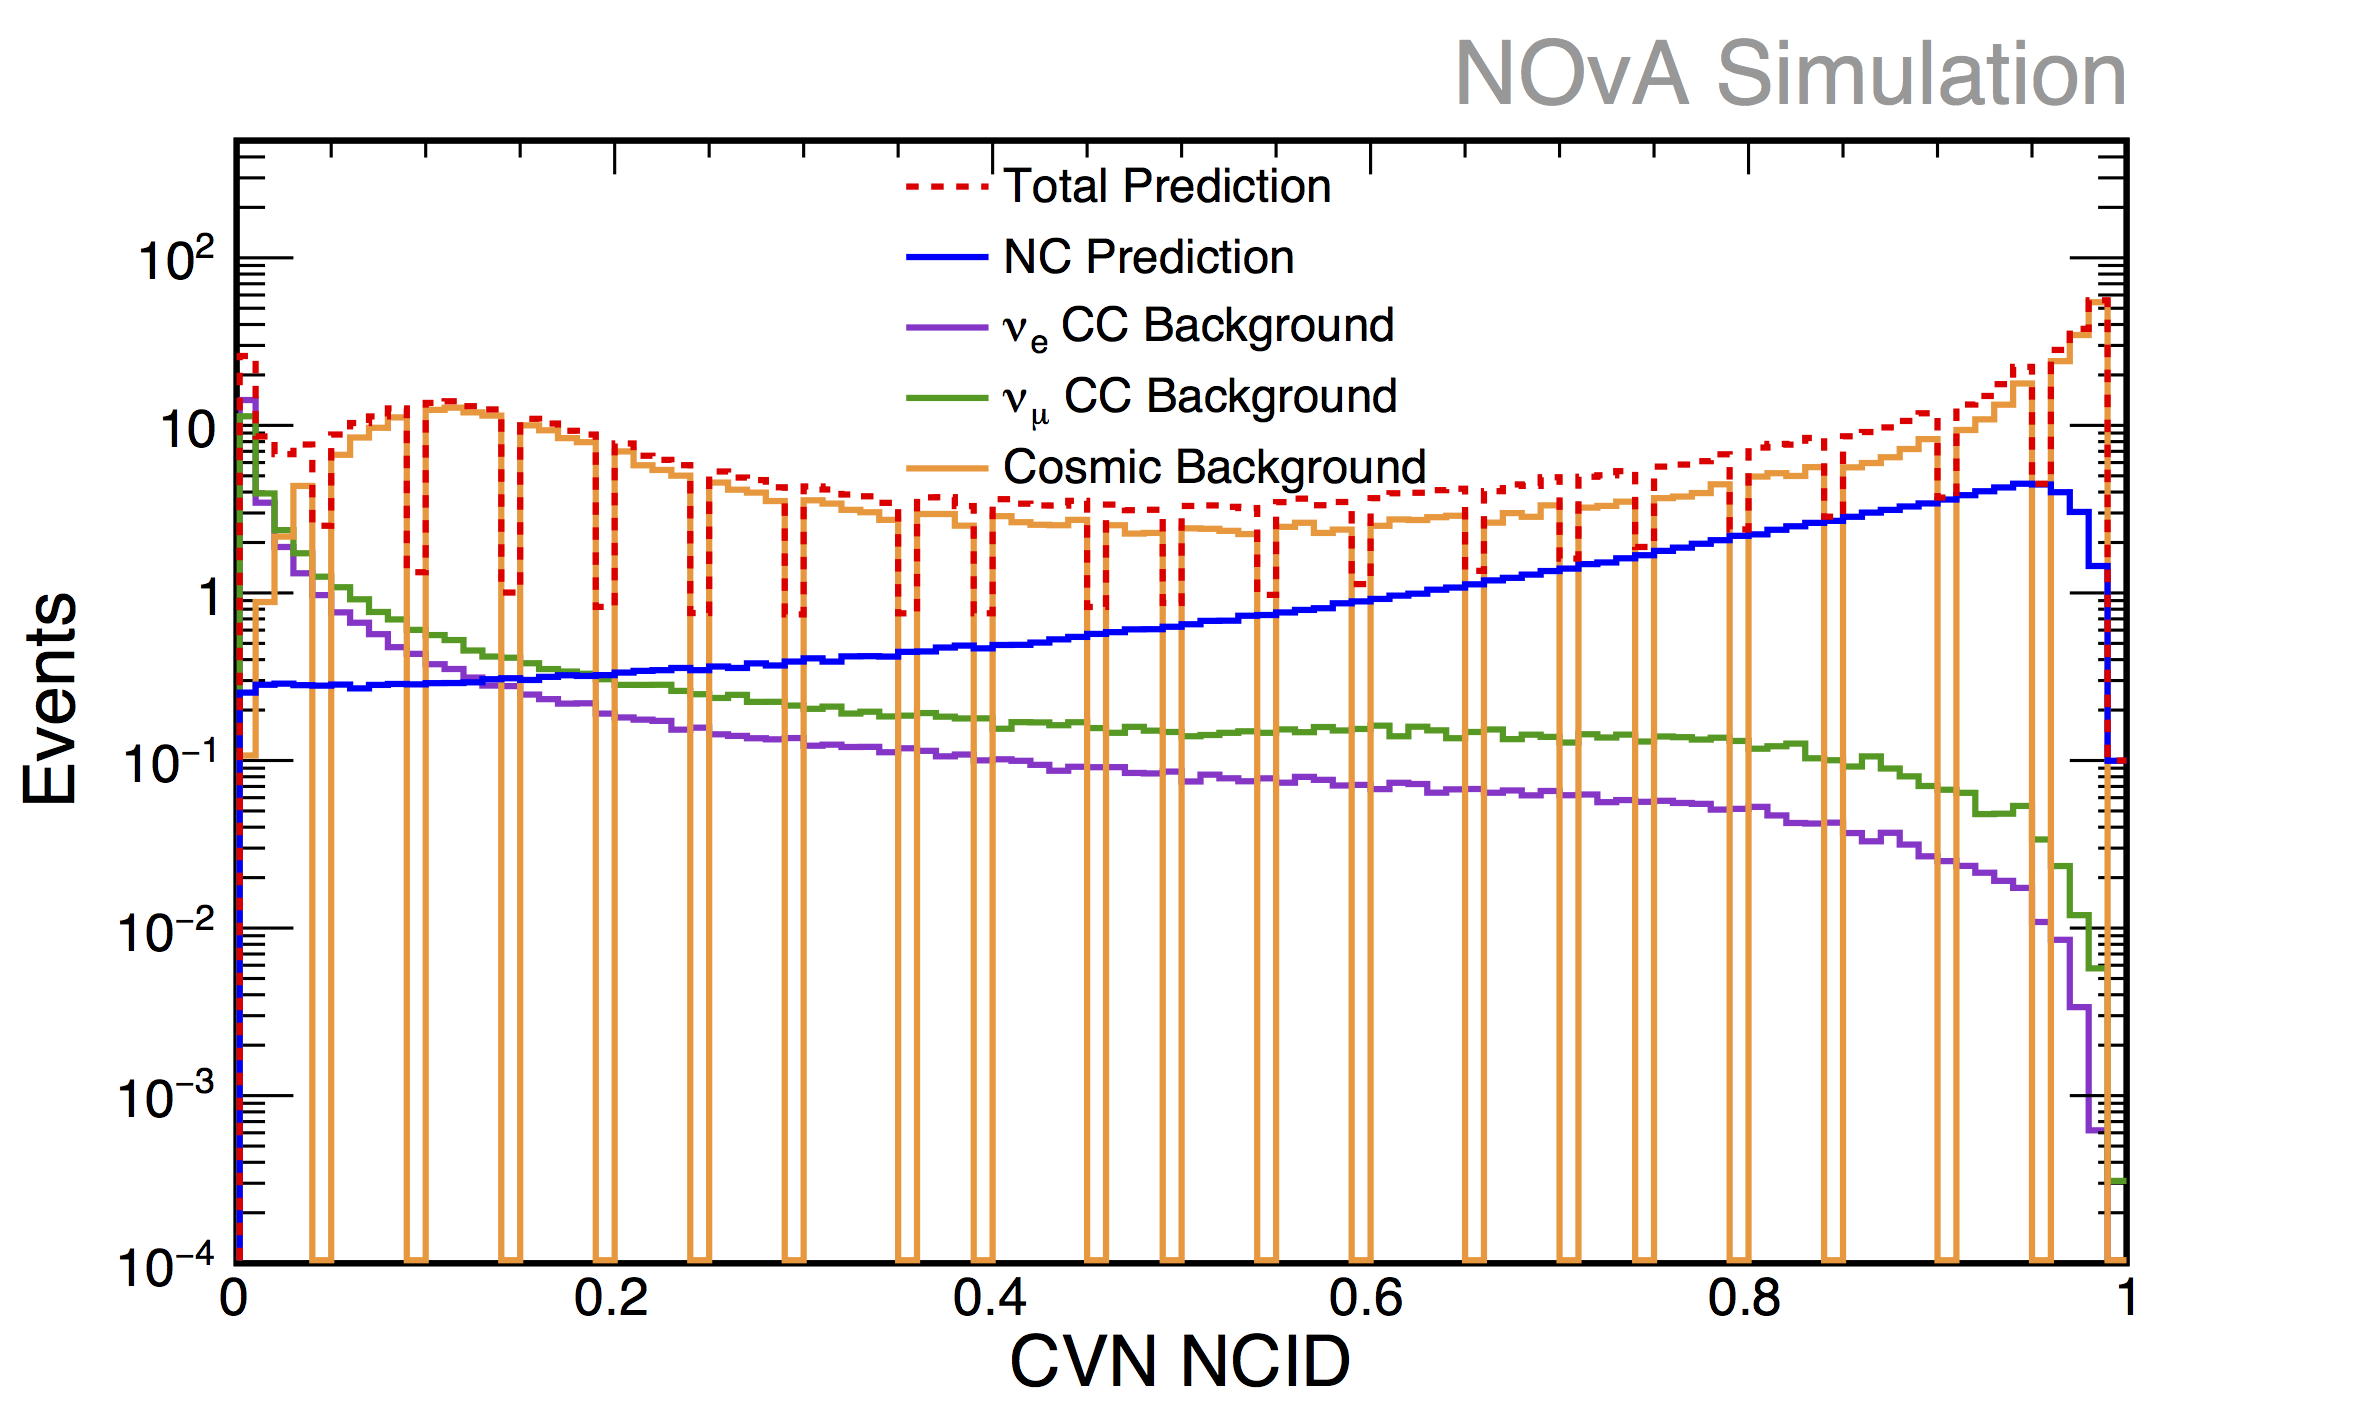
\includegraphics[width=.48\textwidth]{figures/NP1CVNC.png} &
    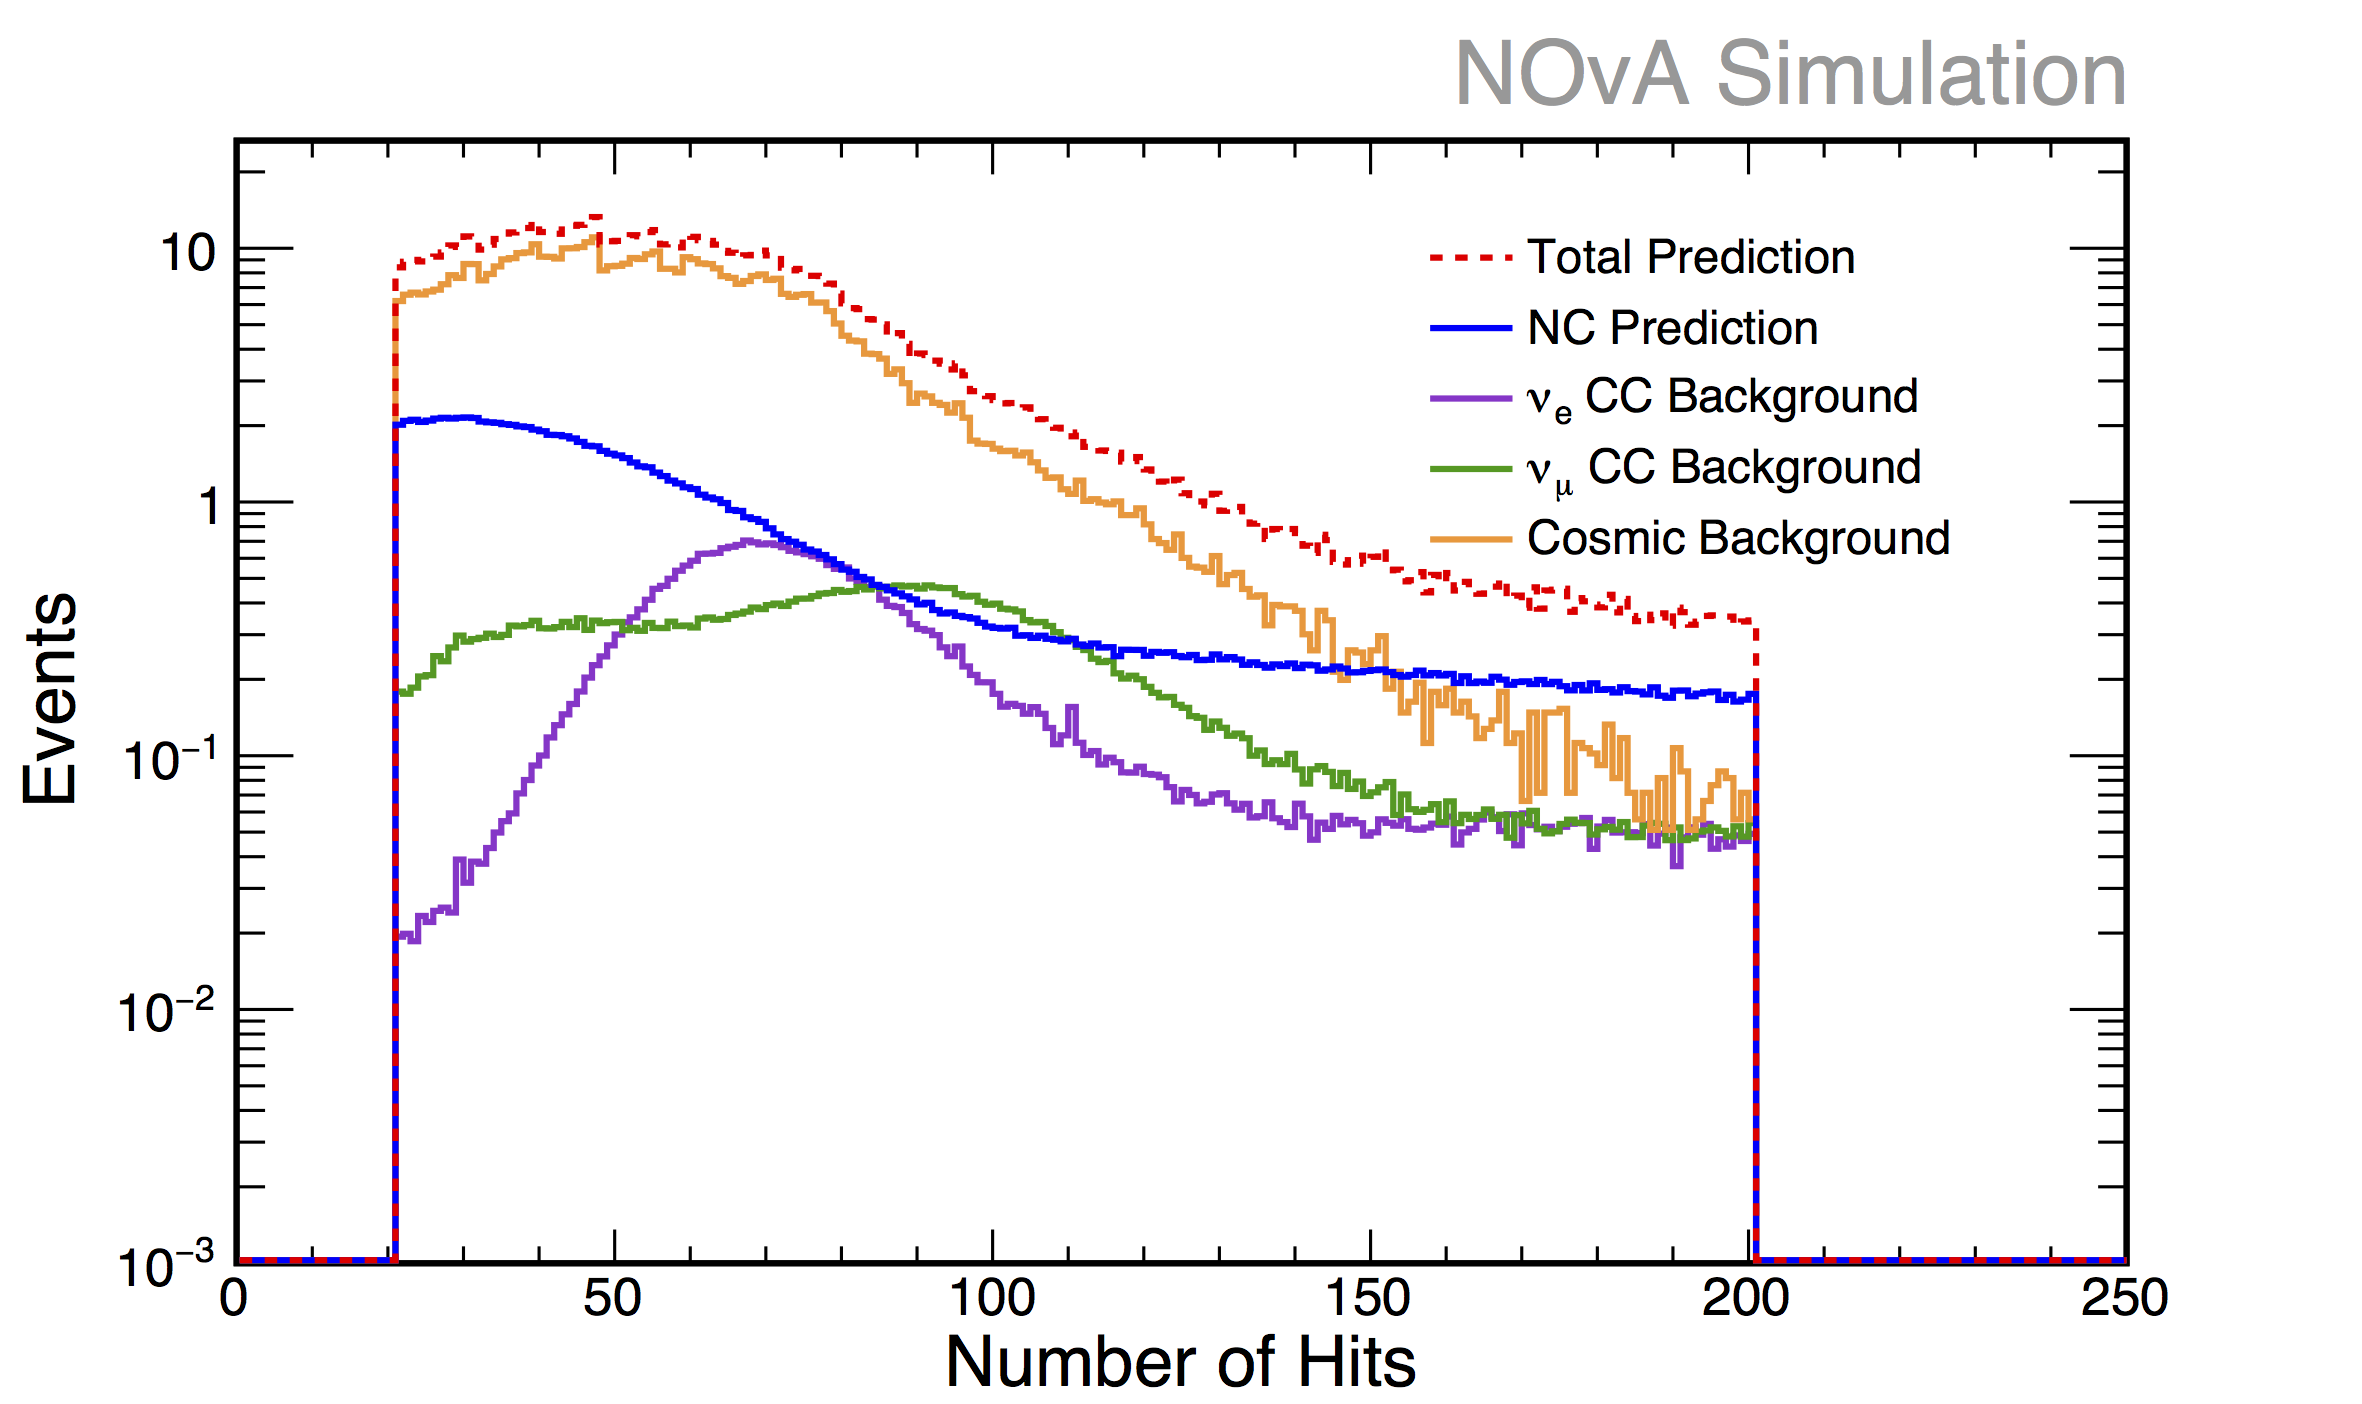
\includegraphics[width=.48\textwidth]{figures/NP1NHit.png} \\
    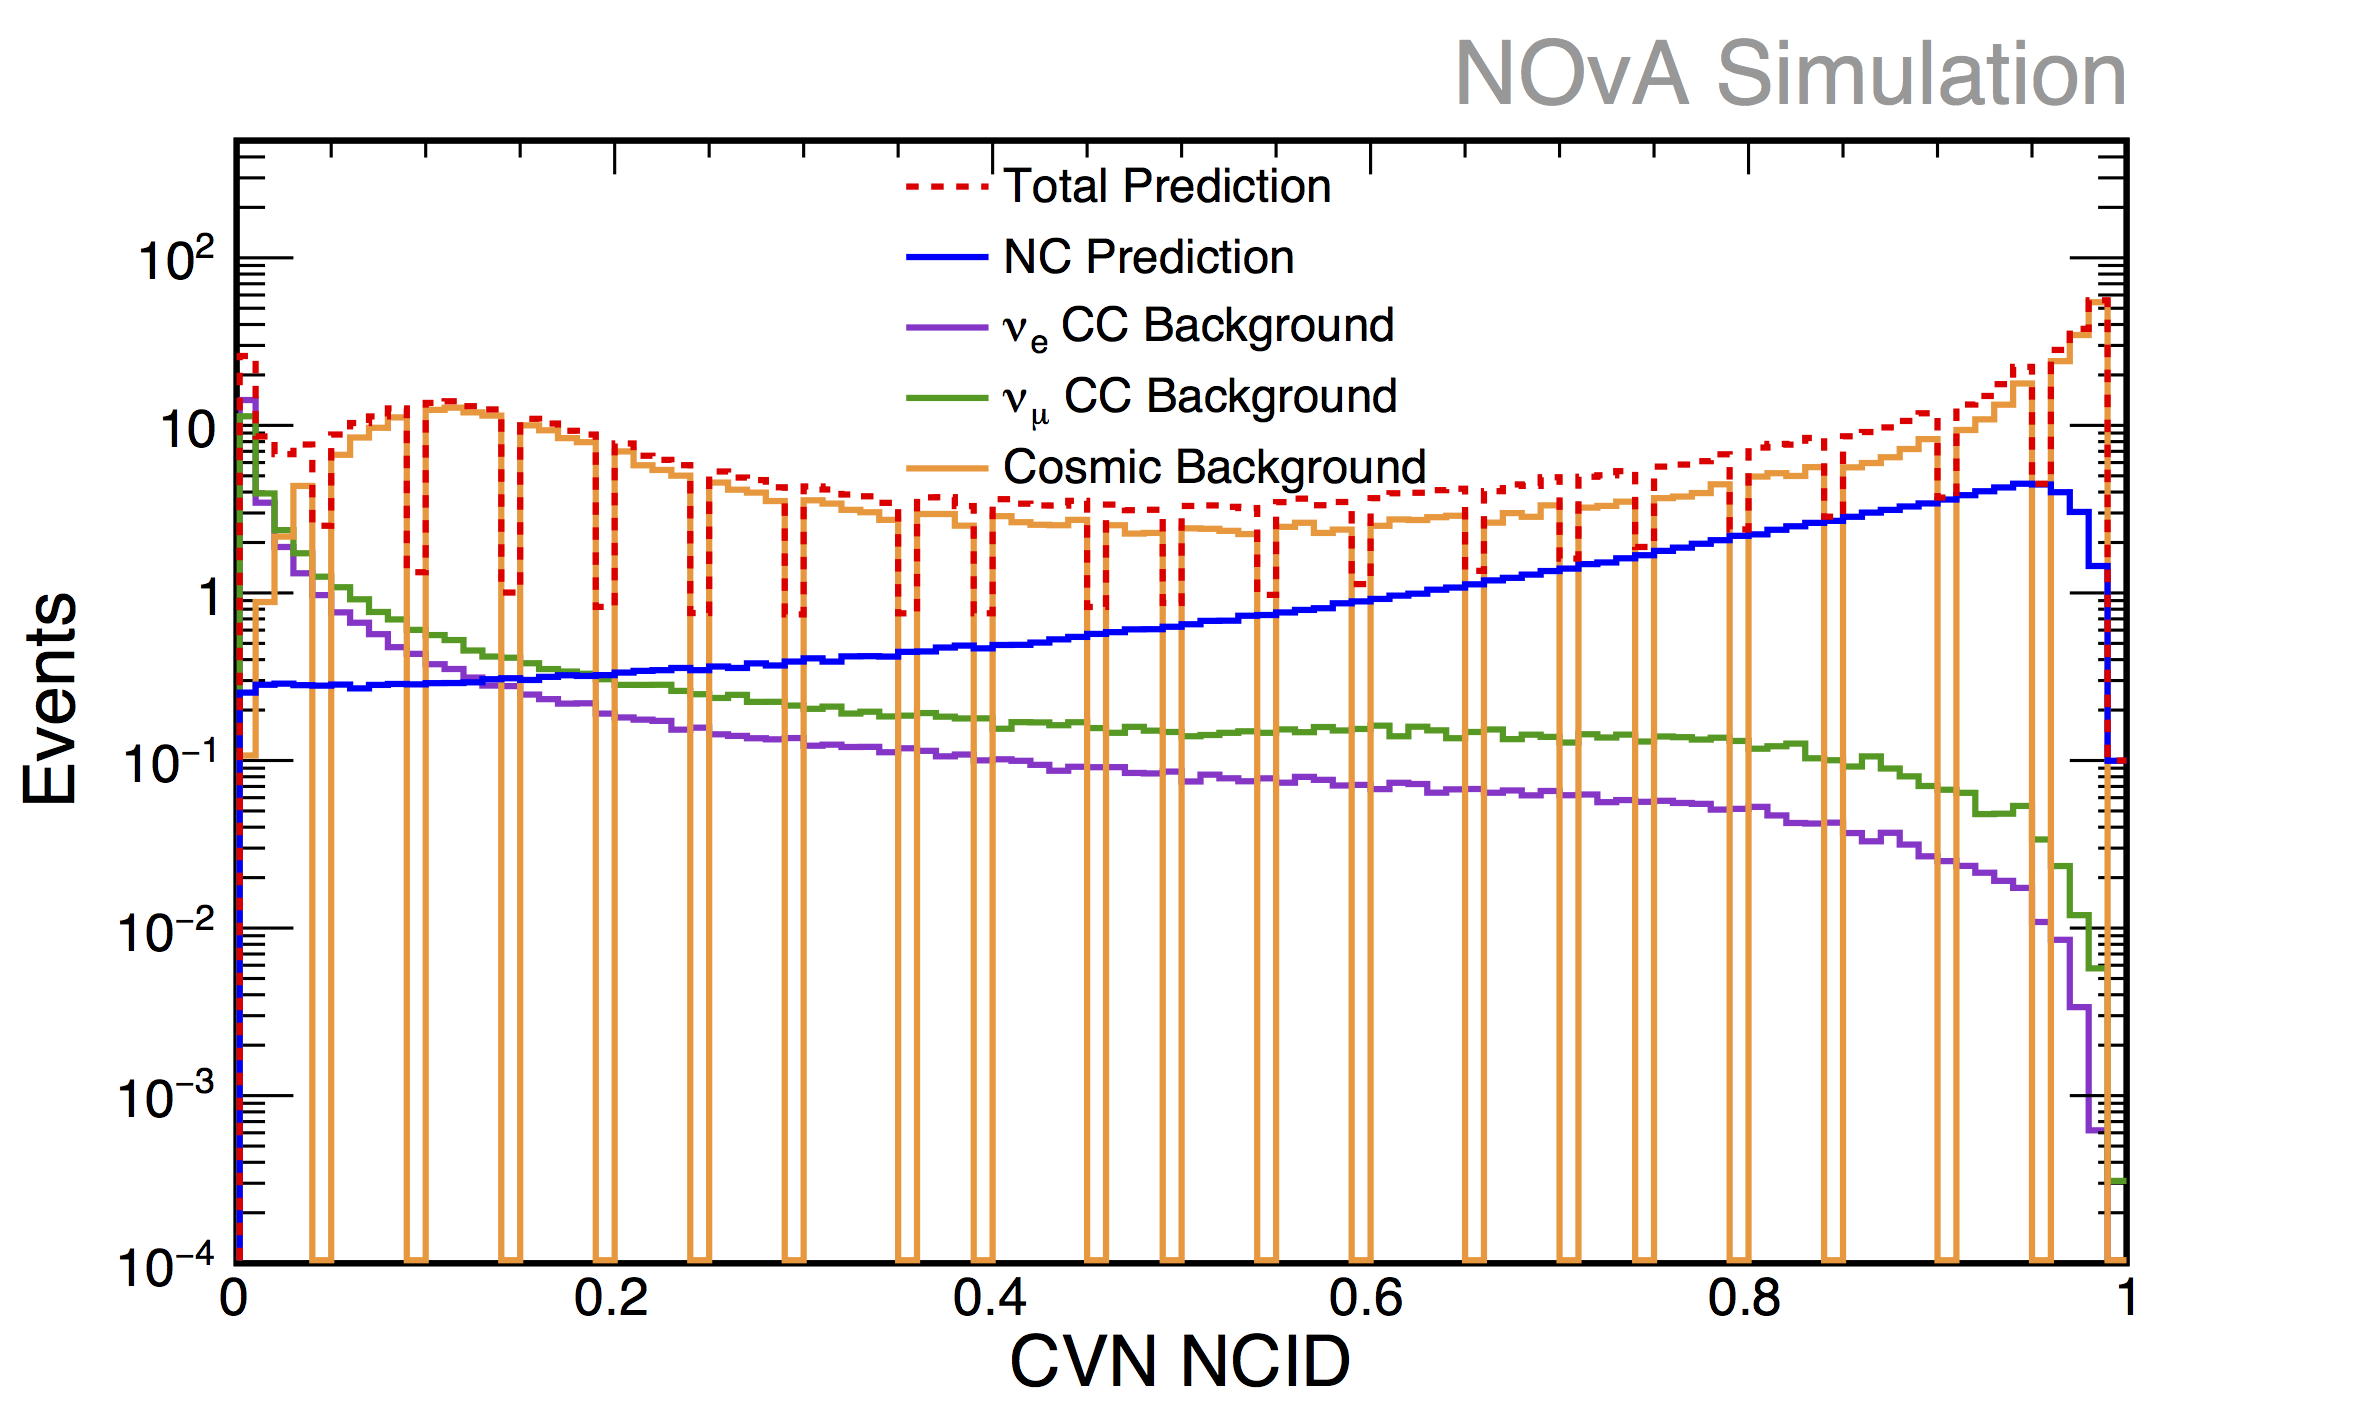
\includegraphics[width=.48\textwidth]{figures/NP1CVNC.png} &
    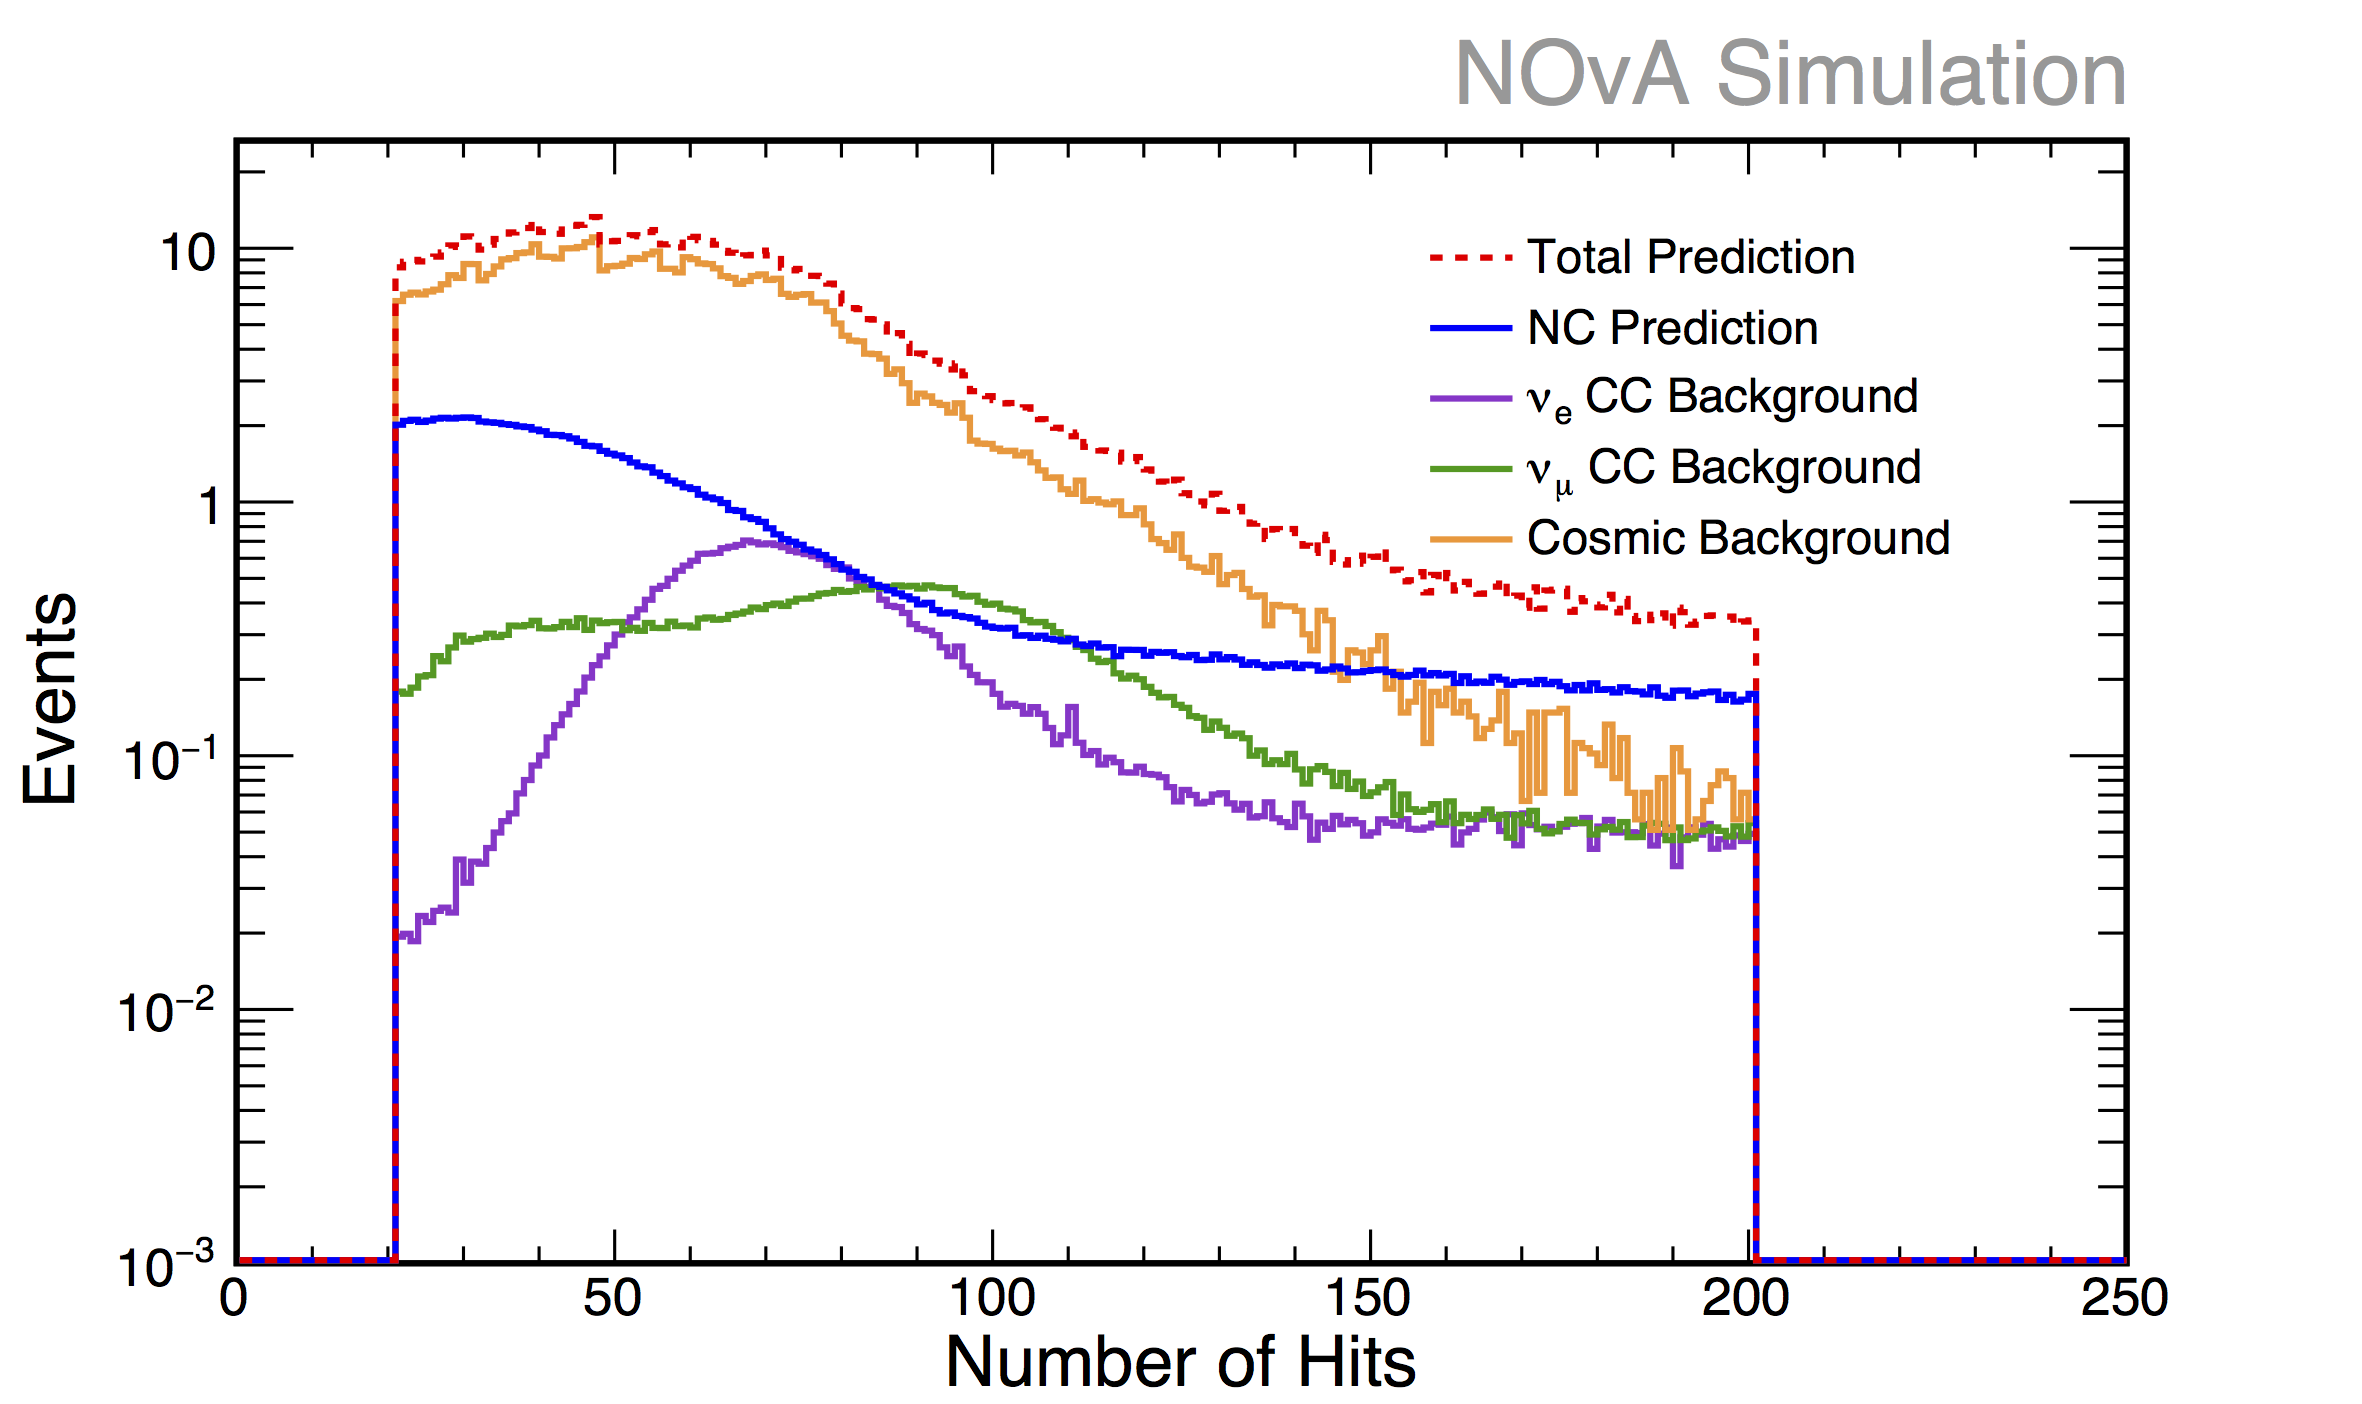
\includegraphics[width=.48\textwidth]{figures/NP1NHit.png} \\
  \end{tabular}
  \caption[RemID and LID Distributions]{Distributions of RemID (left column) and LID (right column) at the FD before (top row) and after (bottom row) applying the cut on CVN listed in Table~\ref{tab:NCSel}.}
  \label{fig:NCSelRemLID}
\end{figure}

The distributions of CVN and the number of hits at the FD are shown in fig.~\ref{fig:NCSel}. Table \ref{tab:NCSel} summarizes the cuts used, table \ref{tab:NP1NCSel} lists the event rates before and after the selection cuts are applied, and fig.~\ref{fig:NP1NCSel} shows the energy distributions of events that pass these cuts.
\begin{figure}[h]
  \centering
  \begin{tabular}{c c}
    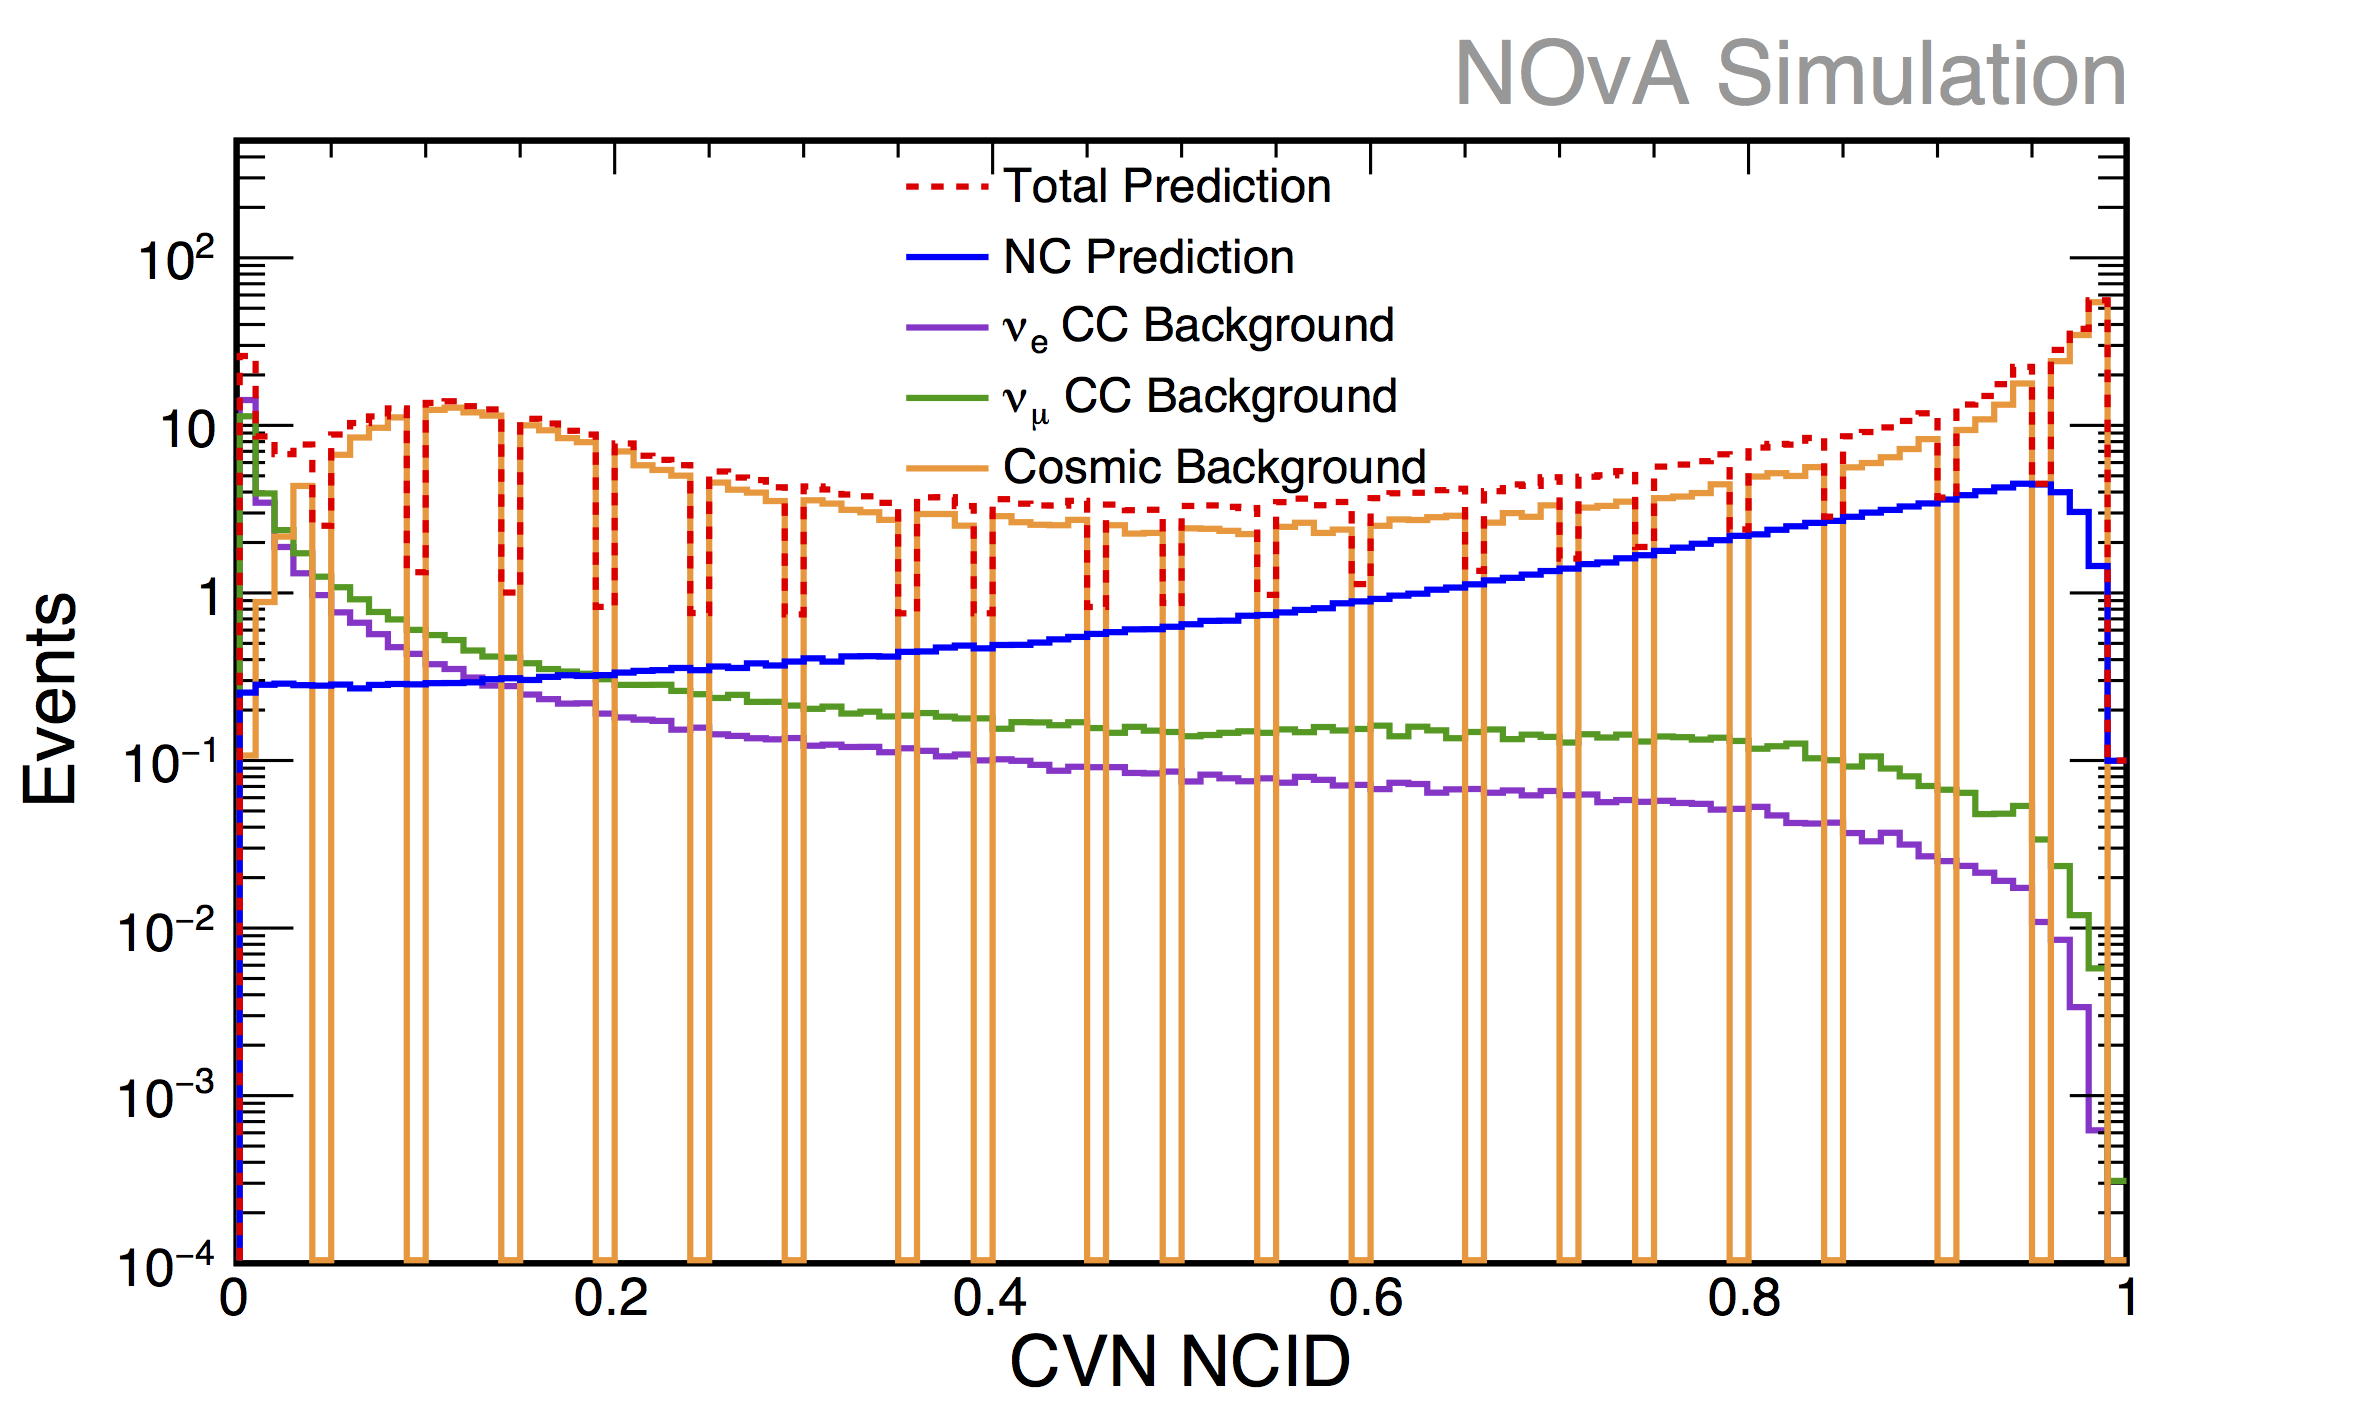
\includegraphics[width=.48\textwidth]{figures/NP1CVNC.png} &
    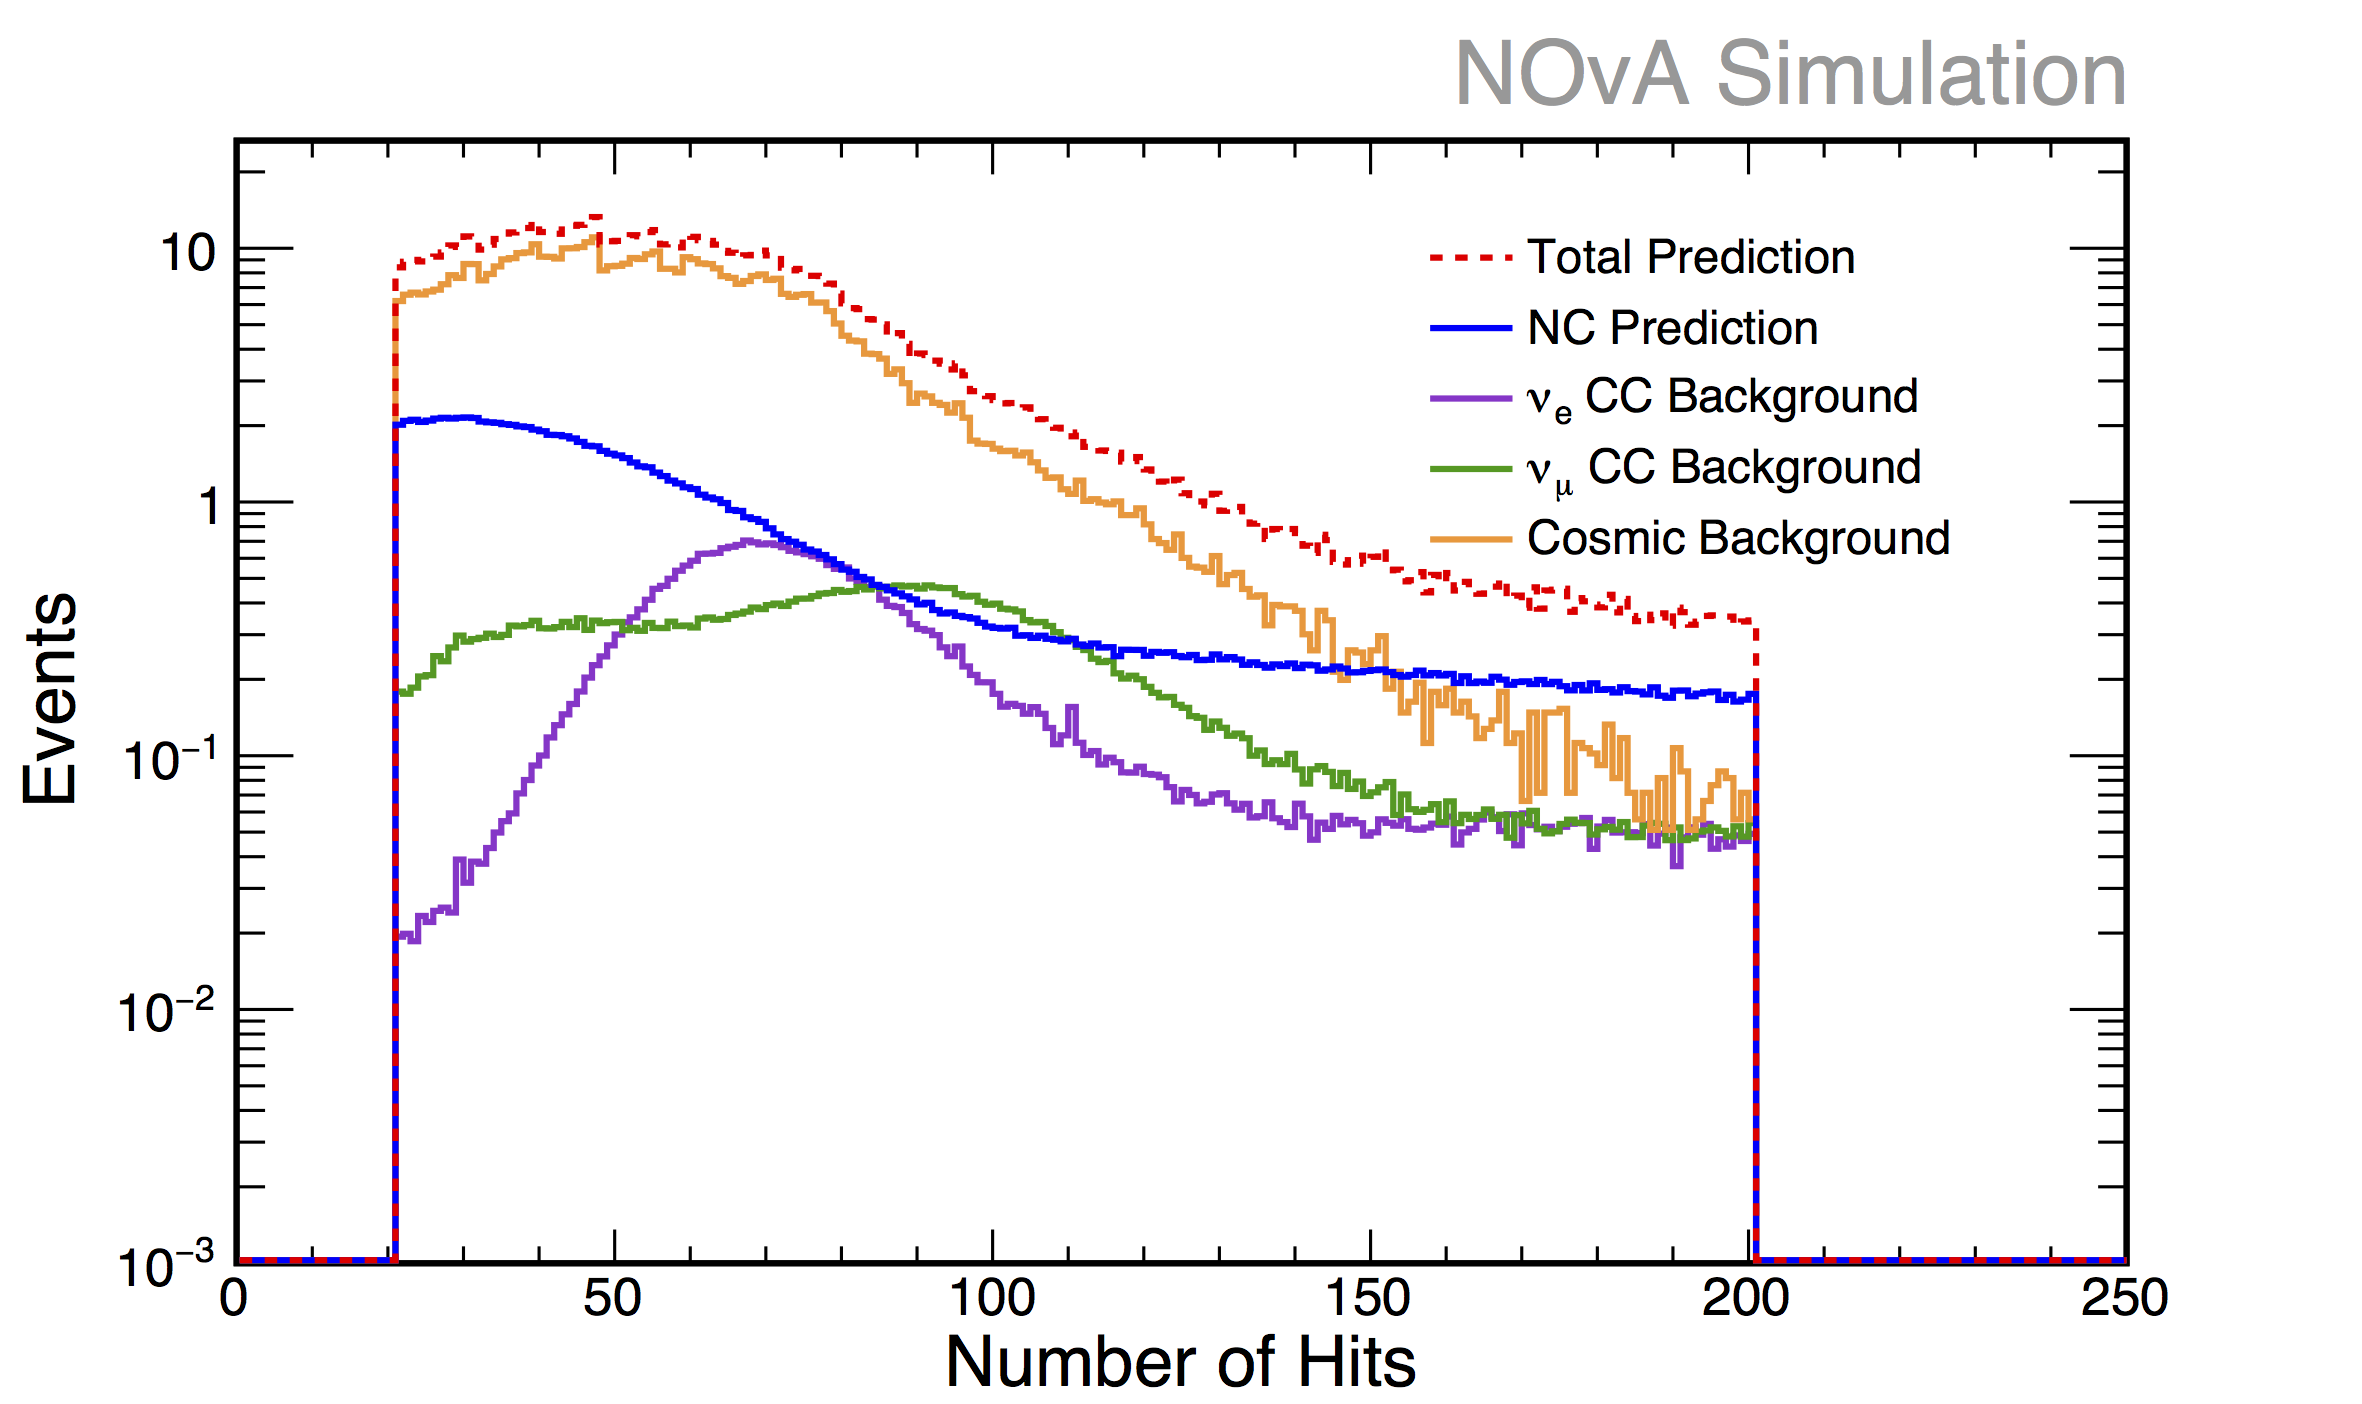
\includegraphics[width=.48\textwidth]{figures/NP1NHit.png} \\
  \end{tabular}
  \caption[NC Selection Variable Distributions]{Distributions of variables used for NC selection at the FD.}
  \label{fig:NCSel}
\end{figure}

\begin{table}[h]
  \begin{center}
    \caption[NC Selection Cuts]{NC selection cuts to reject CC events, leaving a relatively pure sample of NC events.}
    \label{tab:NCSel}
    \begin{tabular}{c c c}
      \hline\hline
      Selection Parameter & Metric for Event to Pass \\
      \hline
      RemID distribution score & $\leq 0.6$ \\
      LID distribution score & $\leq 0.5$ \\
      CVN NC distribution score & $\geq 0.03$ \\
      Number of Hits & $\leq 200$ \\
      \hline
    \end{tabular}
  \end{center}
\end{table}

\begin{table}[h]
  \begin{center}
    \caption[Event Table: NC Selection Cuts]{The number of events before and after application of NC selection cuts, at both detectors.}
    \label{tab:NP1NCSel}
    \begin{tabular}{c c c c c}
      \hline\hline
      Cut Level & NC & $\numu$ CC & $\nue$ CC & Cosmic \\
      \hline
      \multicolumn{5}{l}{FD:} \\
      ...Containment & 113.2 & 39.7 & 31.0 & 580.0 \\
      $+$NC Selection & 94.8 & 12.1 & 7.8 & 200.0 \\
      \multicolumn{5}{l}{ND $(\times 10^{3})$:} \\
      ...Containment & 686.0 & 809.7 & 26.8 & \\
      $+$NC Selection & 593.5 & 360.9 & 9.7 & \\
      \hline
    \end{tabular}
  \end{center}
\end{table}

\begin{figure}[h]
  \centering
  \begin{subfigure}{.48\textwidth}
    \centering
    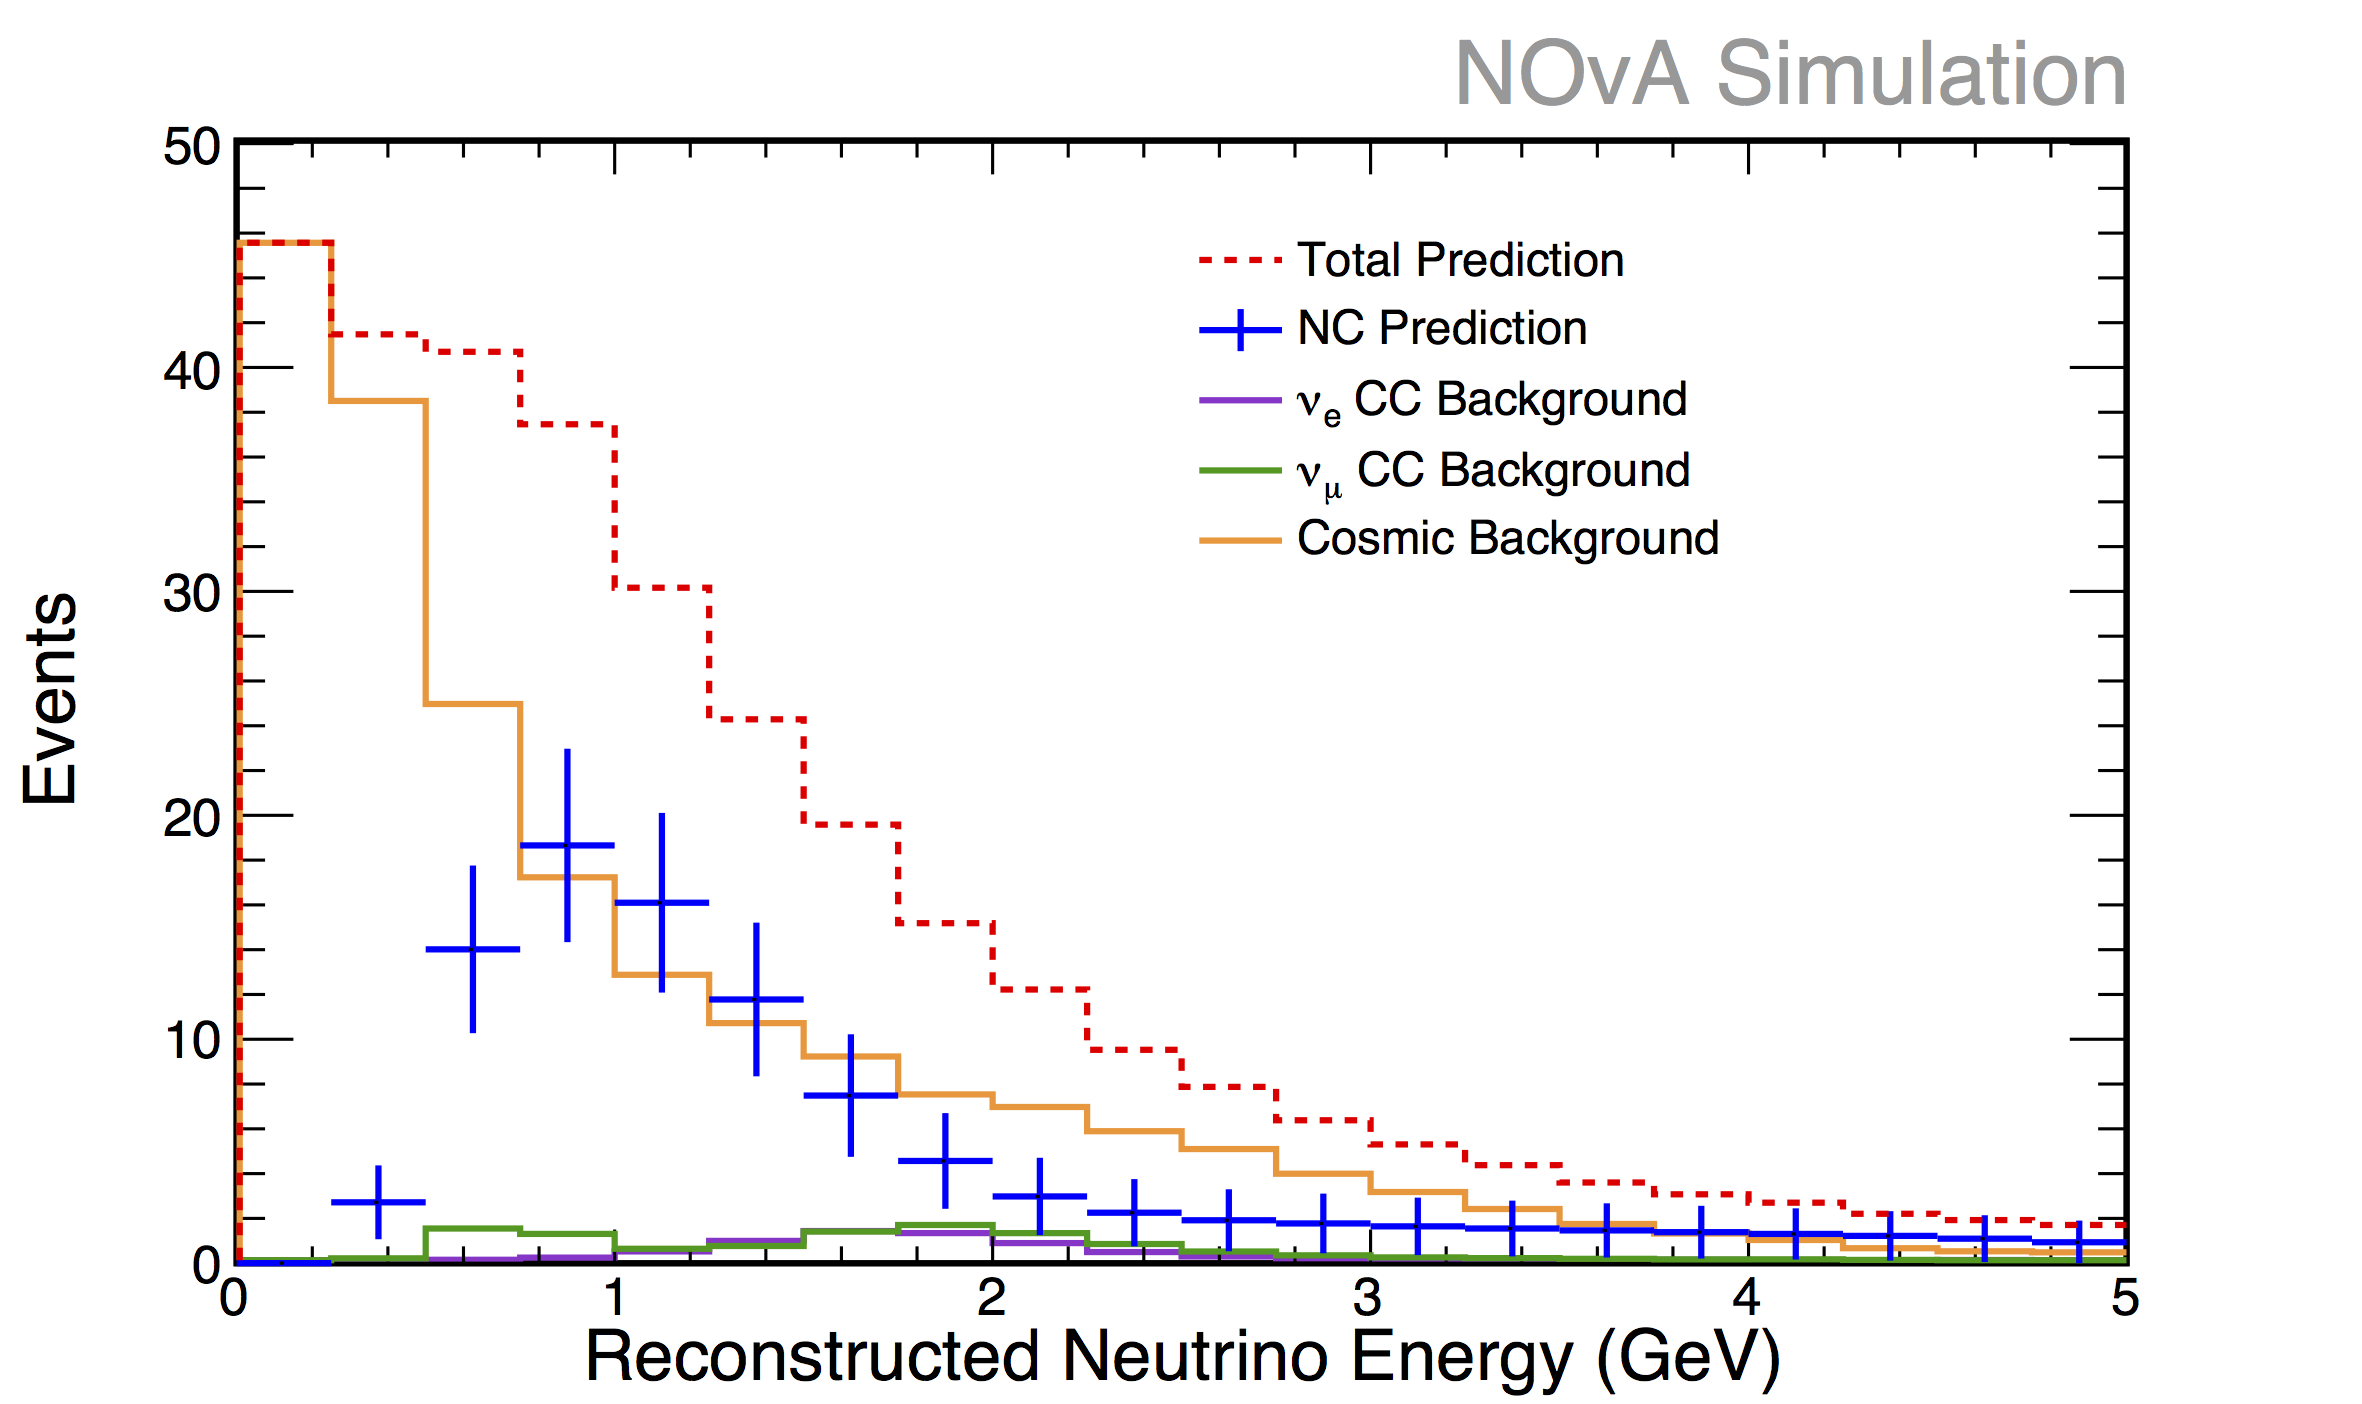
\includegraphics[width=1\linewidth]{figures/RecoE5FD.png}
  \end{subfigure}
  \begin{subfigure}{.48\textwidth}
    \centering
    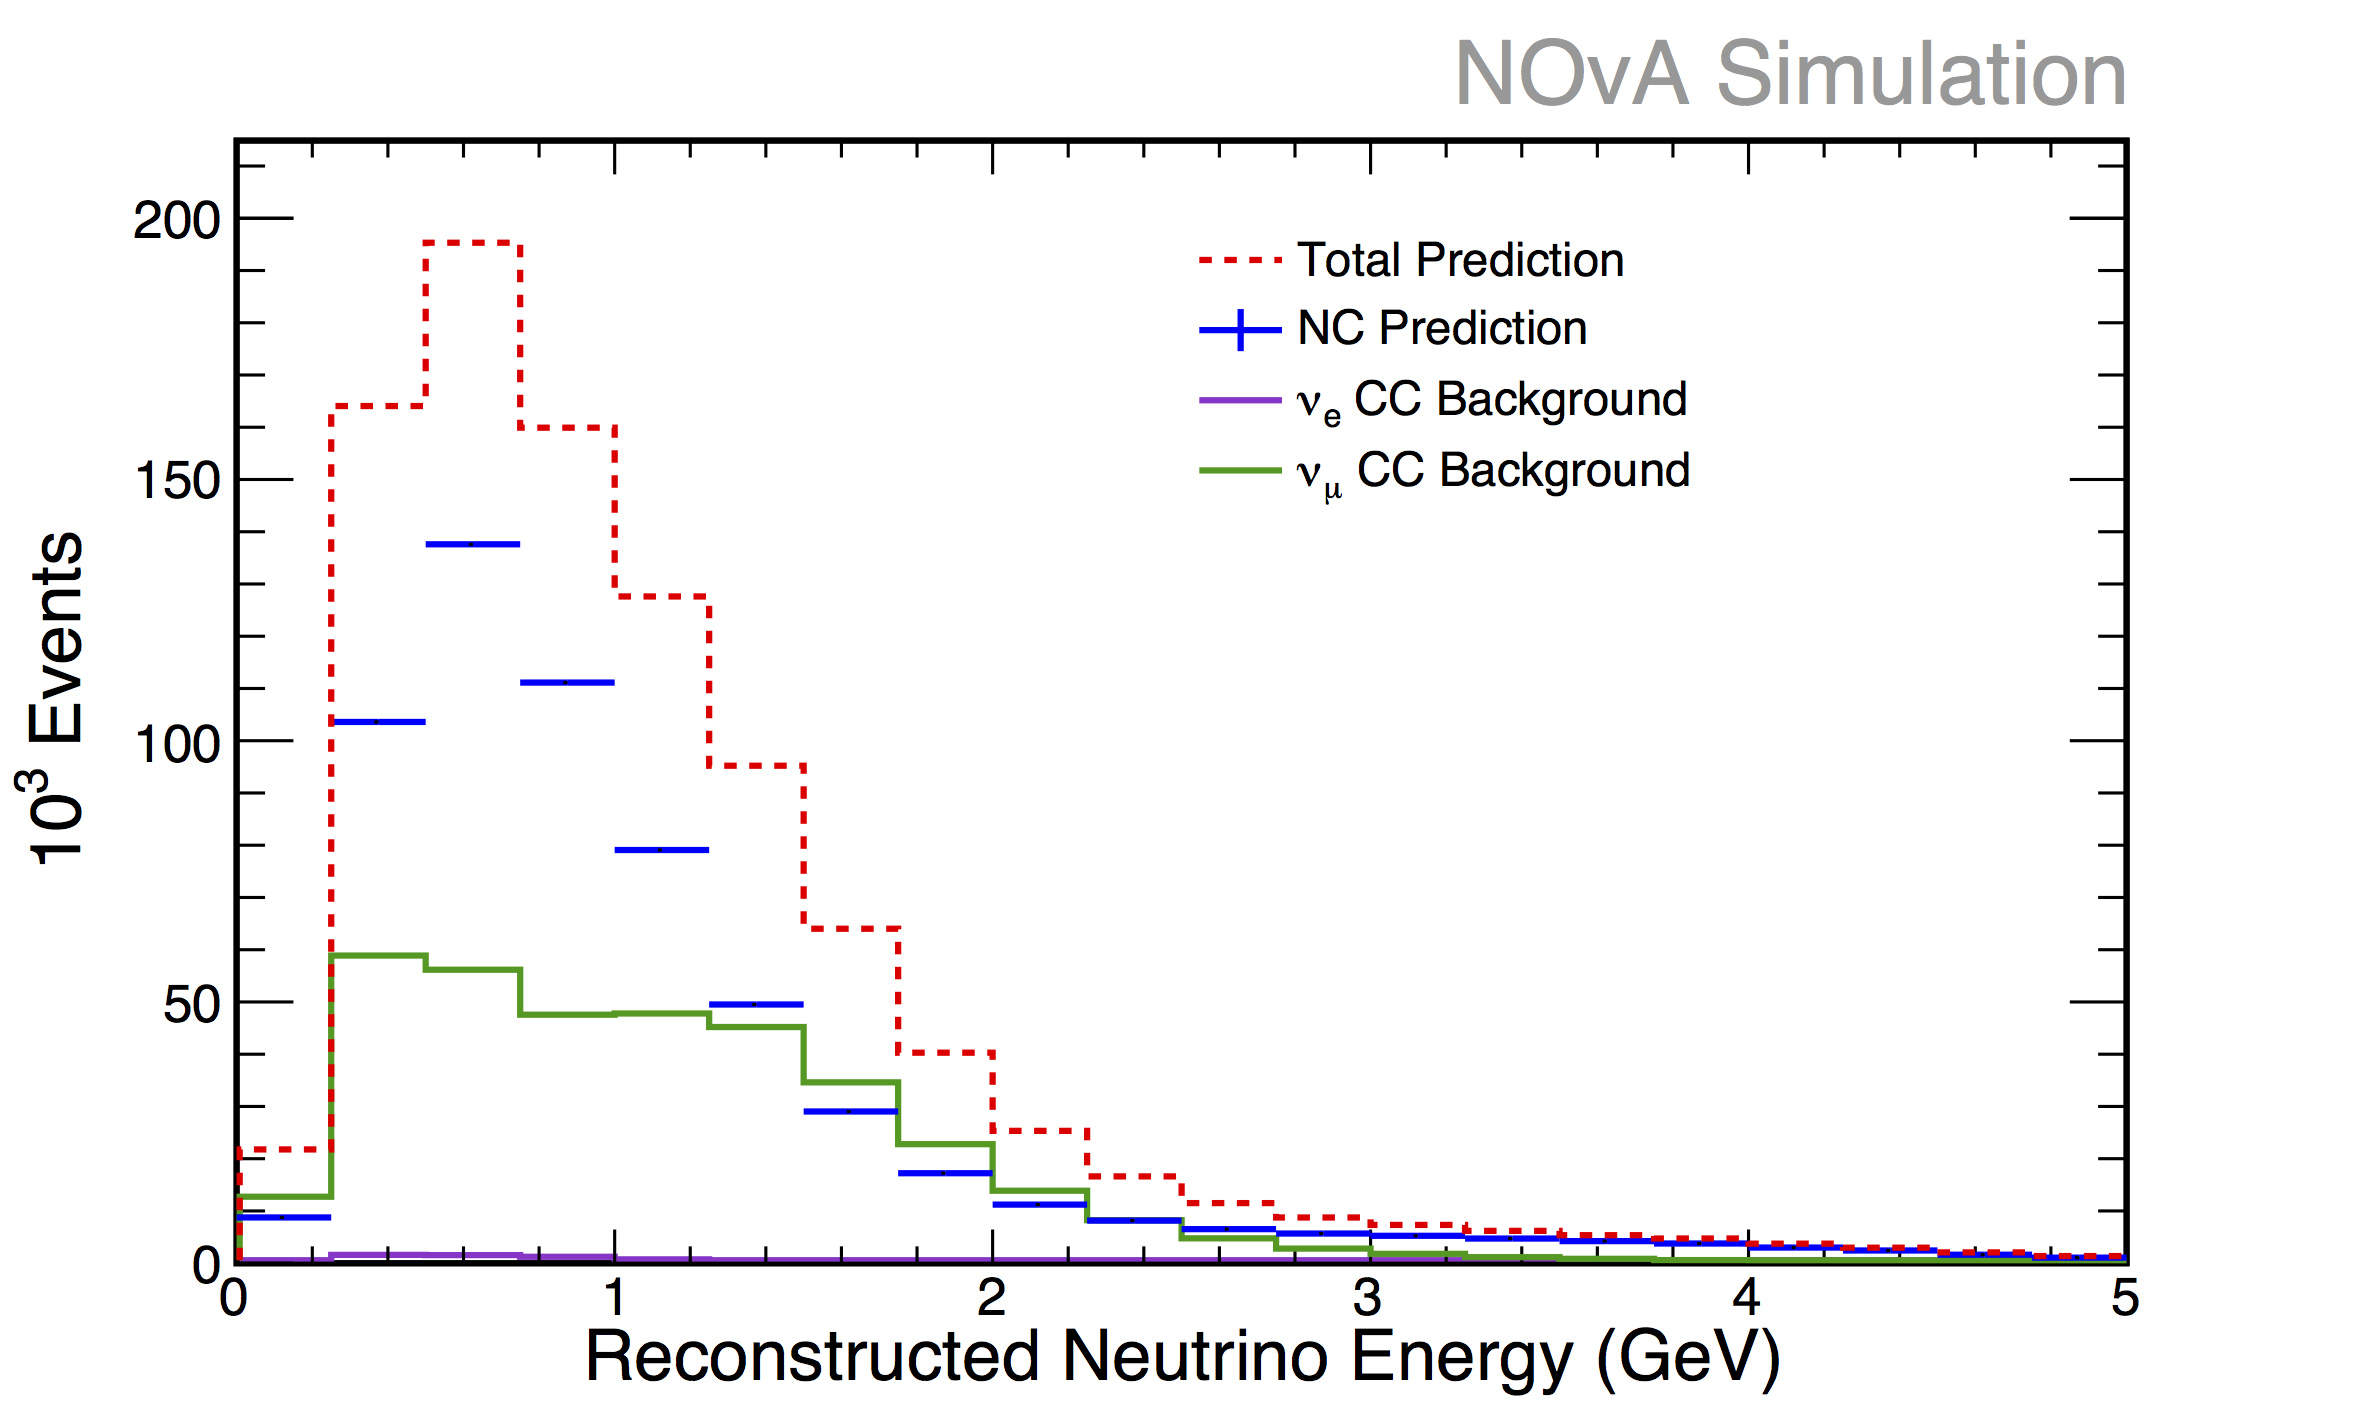
\includegraphics[width=1\linewidth]{figures/RecoE5ND.png}
  \end{subfigure}
  \caption[Energy Spectra After NC Selection Cuts]{Energy spectra after NC selection cuts for the FD (left) and ND (right).}
  \label{fig:NP1NCSel}
\end{figure}

\section{Cosmic Rejection}

The final set of cuts applied to the events is cosmic rejection. While there are essentially no cosmic events at the ND, the cuts are still applied at the ND when possible to maintain similar spectra at both detectors. The main variable to discriminate against cosmics is the output of a boosted decision tree originally tuned for the $\numu$ disappearance analysis \cite{ref:TNNumuContPID}. This algorithm takes a number of inputs, mainly based on the reconstructed track, such as the angle from the beam, the track length, and number of hits in the track. Another powerful discriminant is the fraction of total transverse energy deposition versus total event energy deposition, originally developed for the $\nue$ appearance analysis \cite{ref:EQNuEFD}. The other cuts used for cosmic rejection are a cut on low average energy per hit, a harsher cut on the start/stop distance of the leading prong to the top of the detector, and removing events where the leading shower has a greatest likelihood of being a muon. The distributions of these variables at the FD are shown in fig.~\ref{fig:CosRej} and Table \ref{tab:CosRej} summarizes the cosmic rejection with the values used for the actual cuts. Table \ref{tab:NP1Cosmic} lists the event rates before and after the cosmic rejection cuts are applied, and fig.~\ref{fig:NP1Cosmic} shows the energy distributions of events that pass these cuts.
\begin{figure}[h]
  \centering
  \begin{tabular}{c c}
    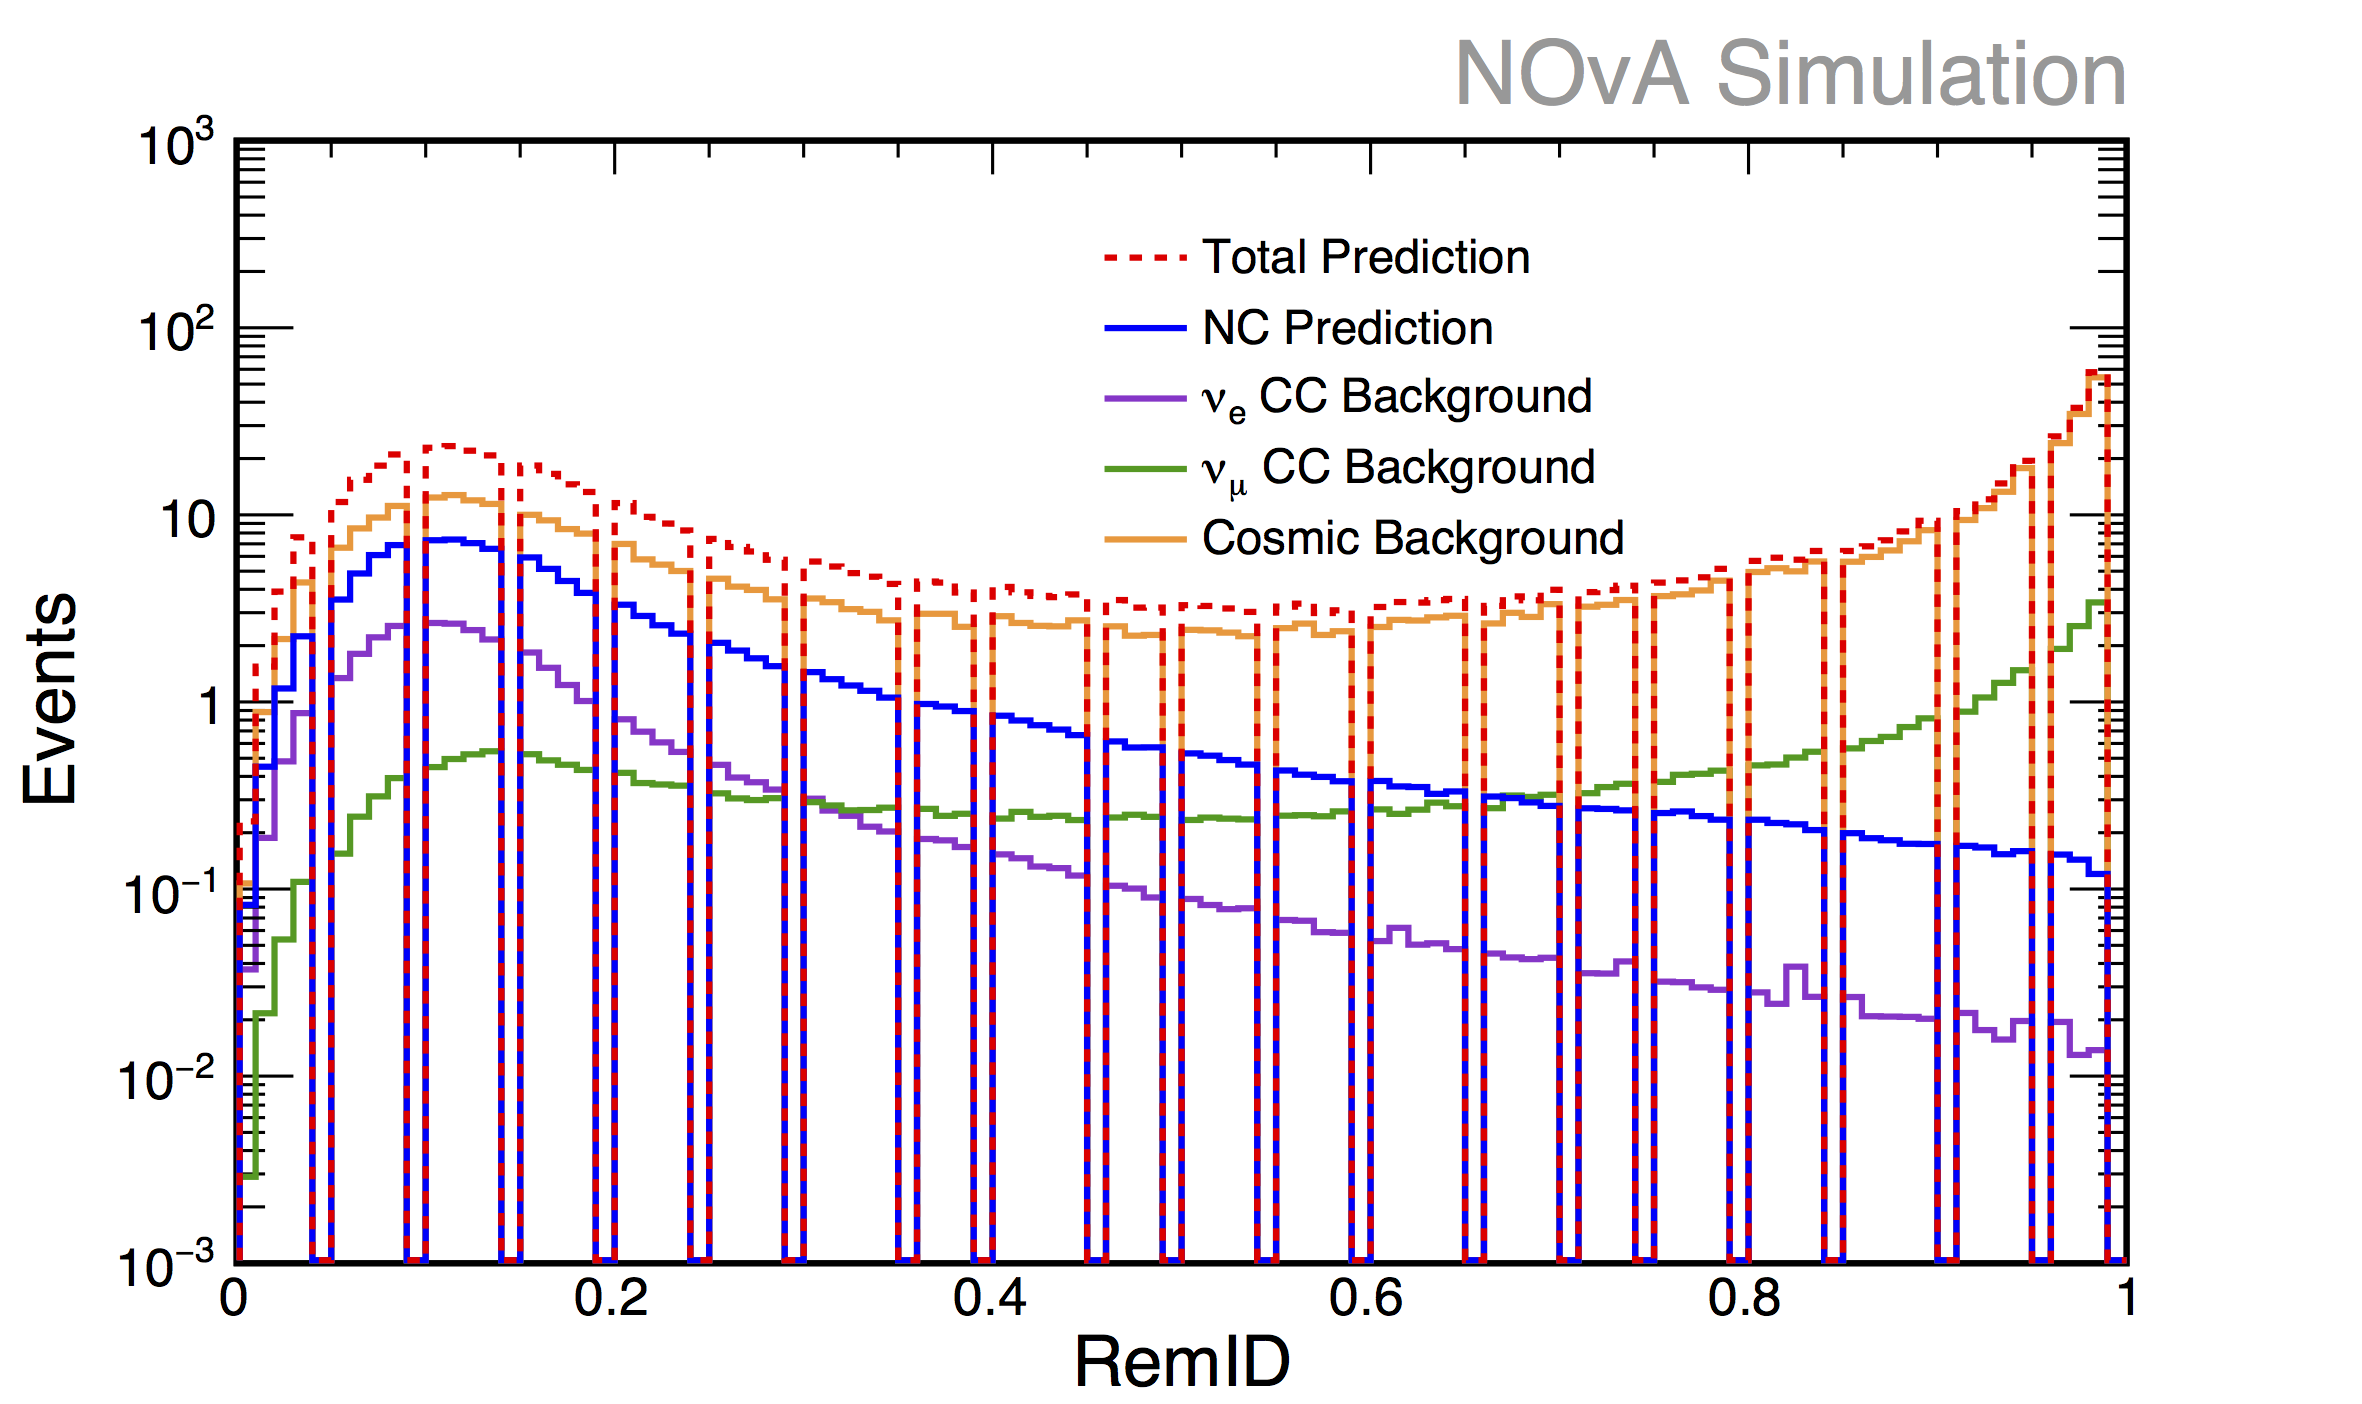
\includegraphics[width=.48\textwidth]{figures/NP1RmID.png} &
    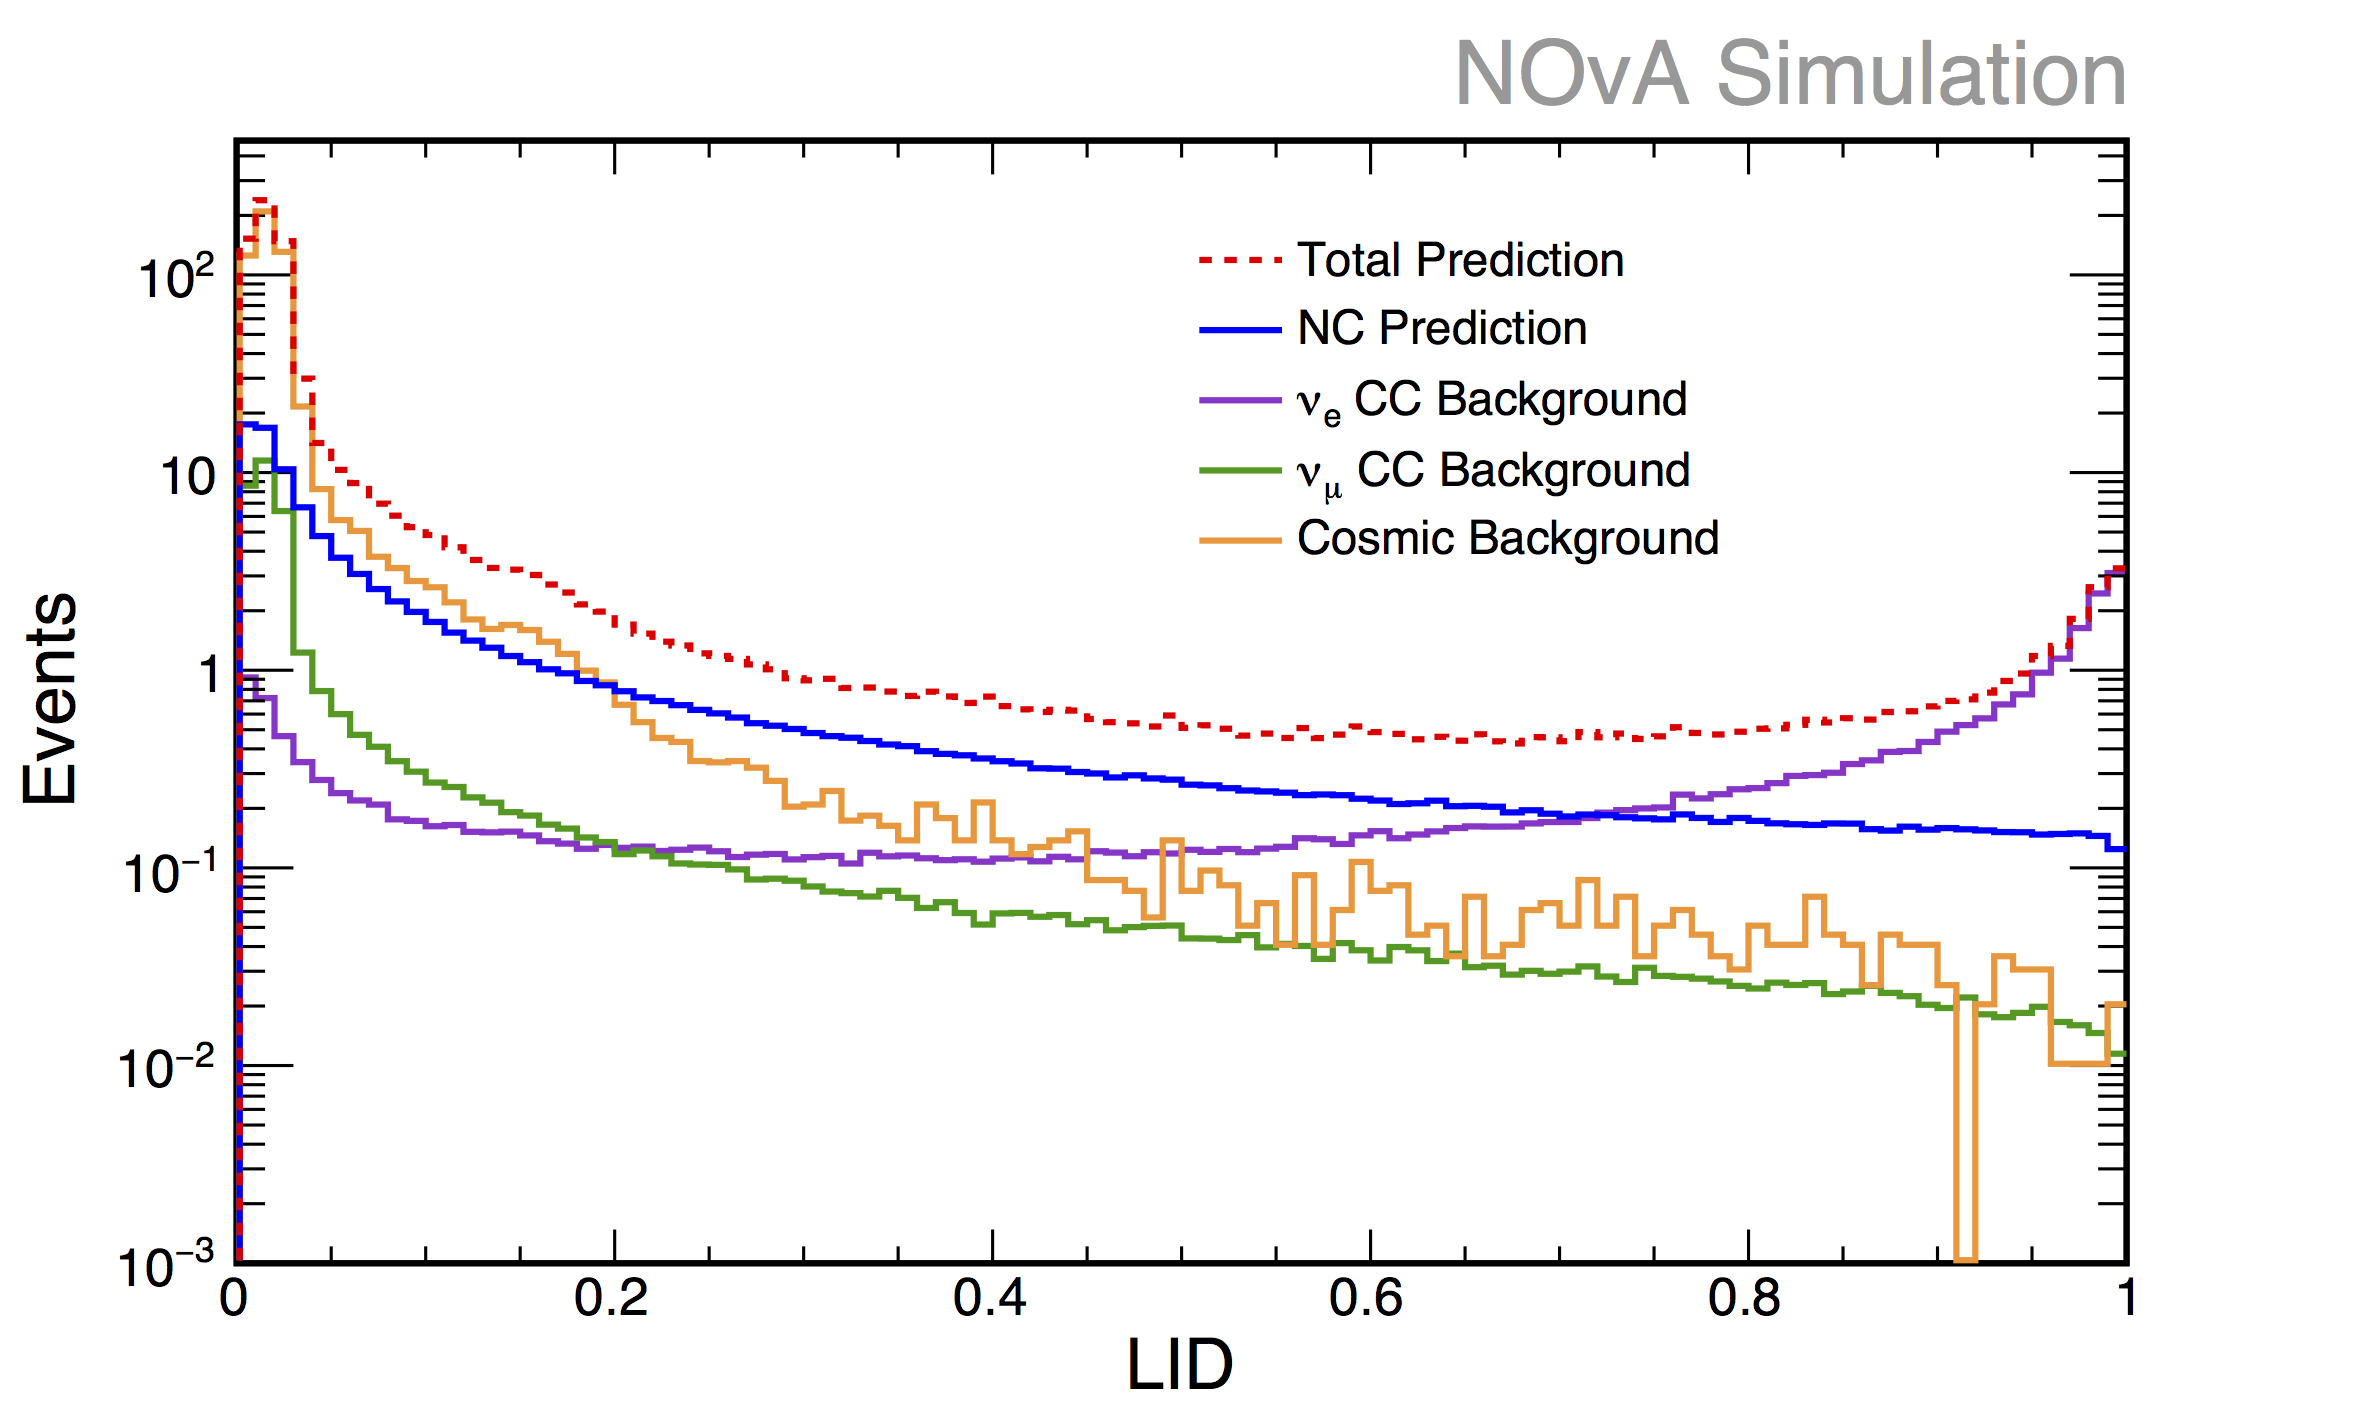
\includegraphics[width=.48\textwidth]{figures/NP1ELID.png} \\
    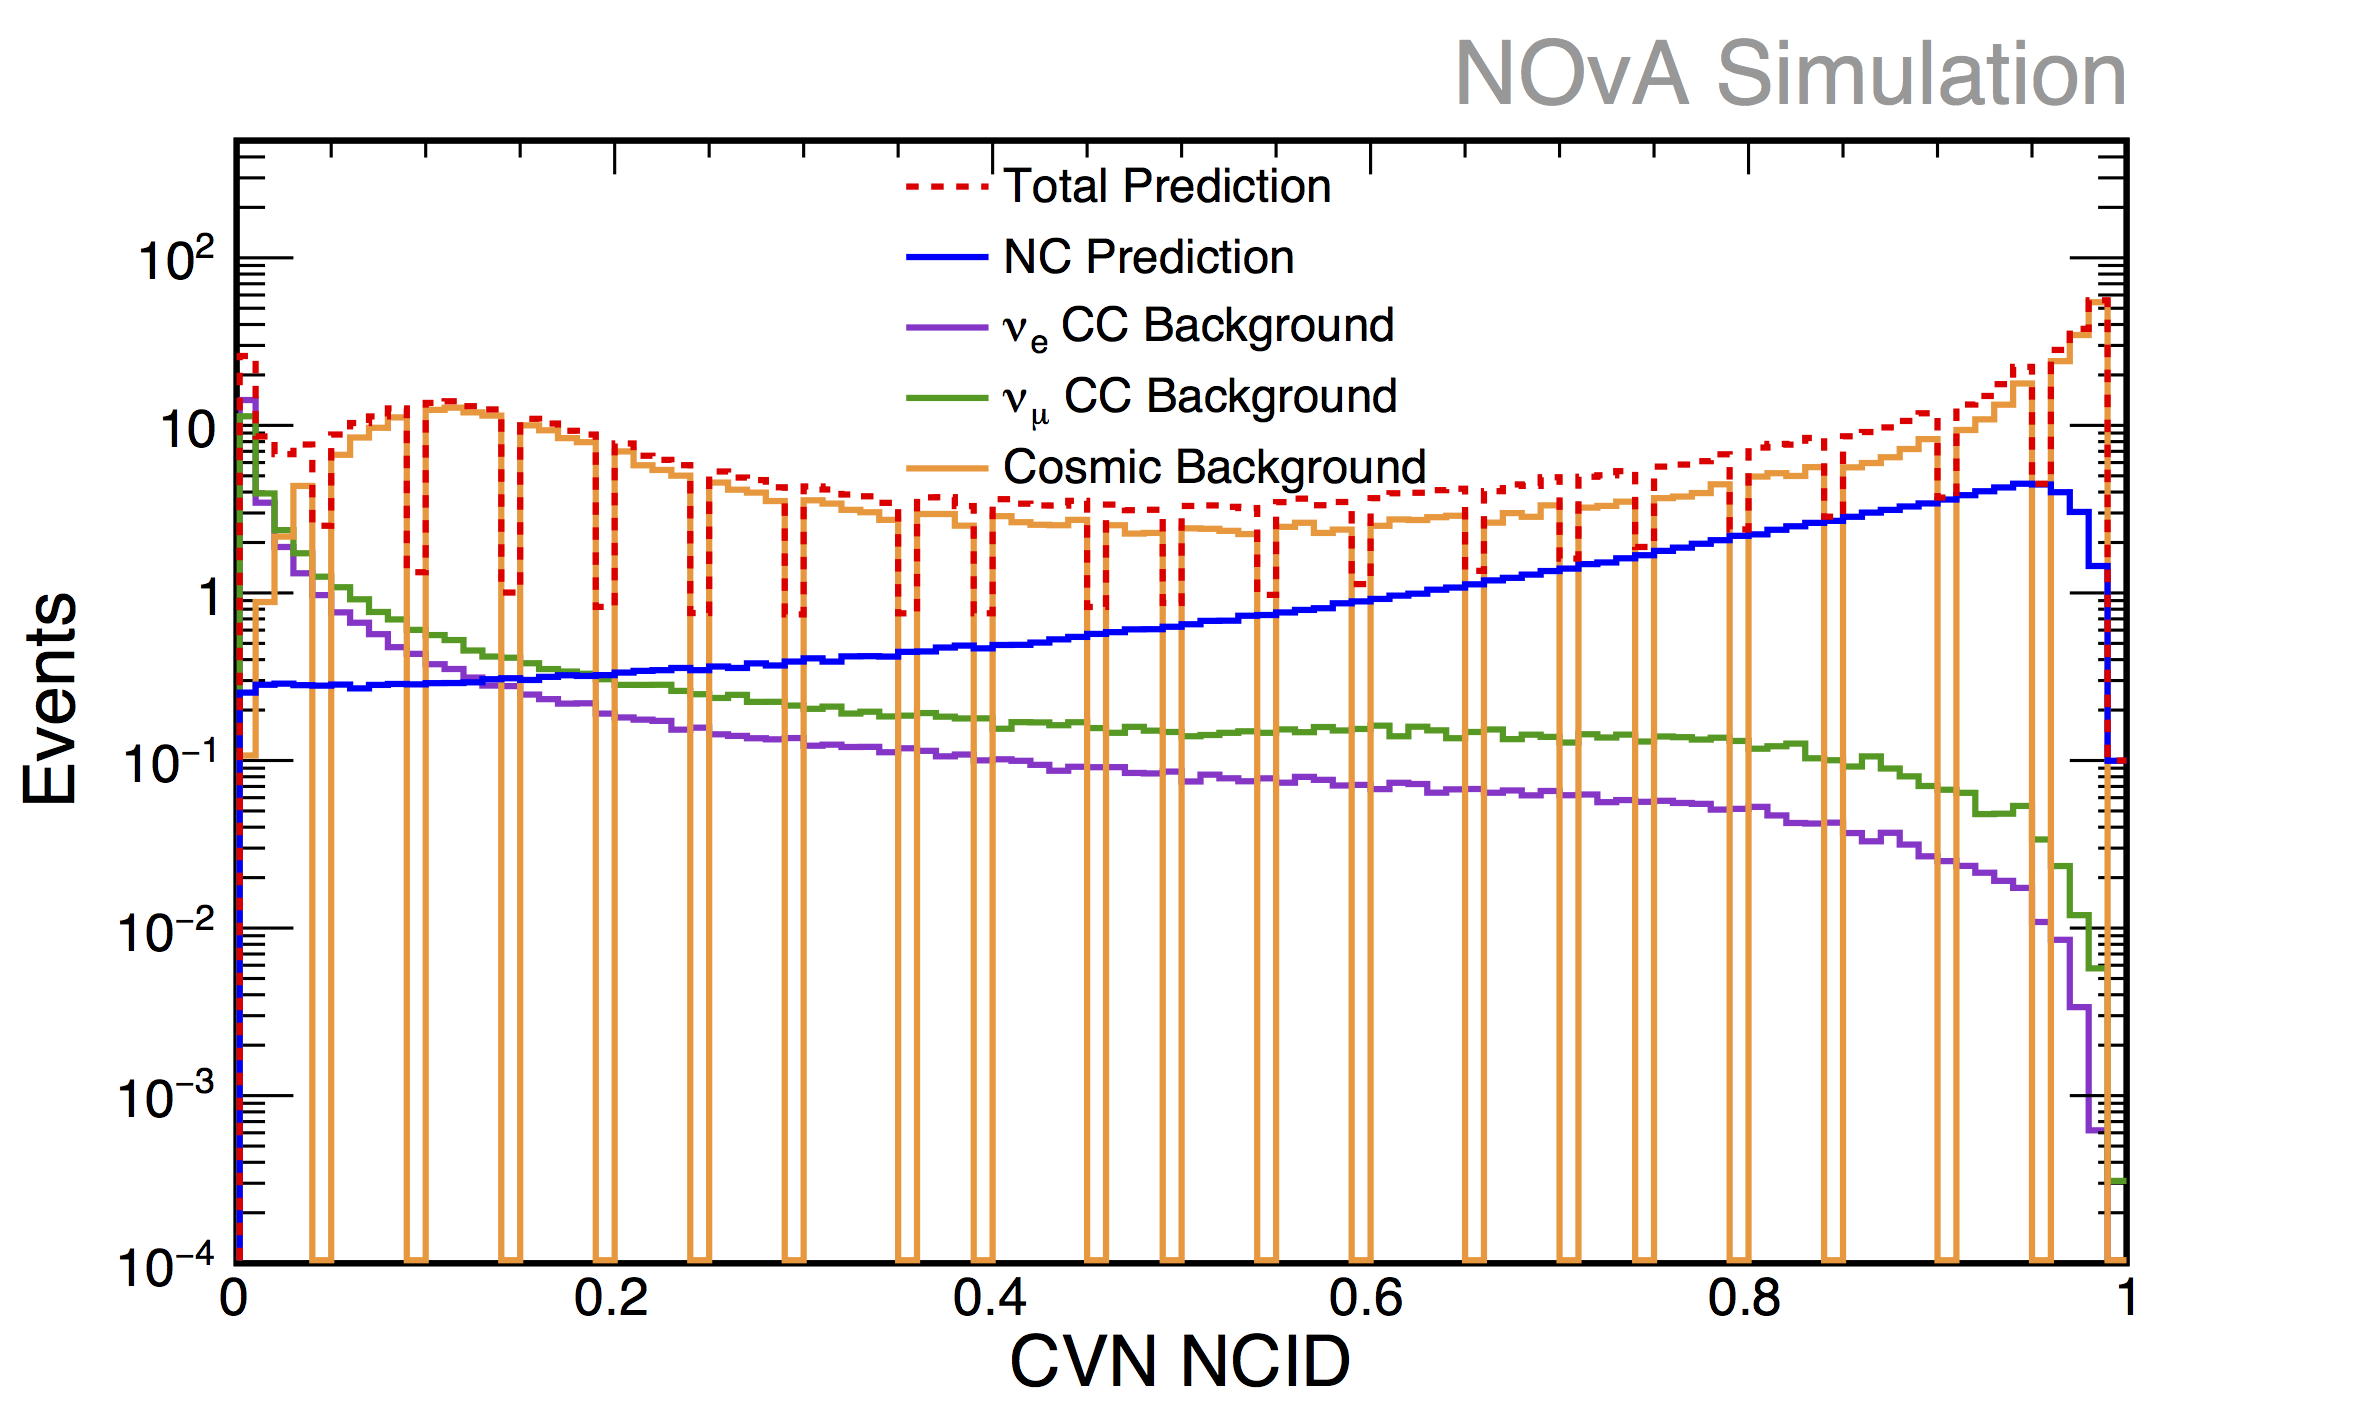
\includegraphics[width=.48\textwidth]{figures/NP1CVNC.png} &
    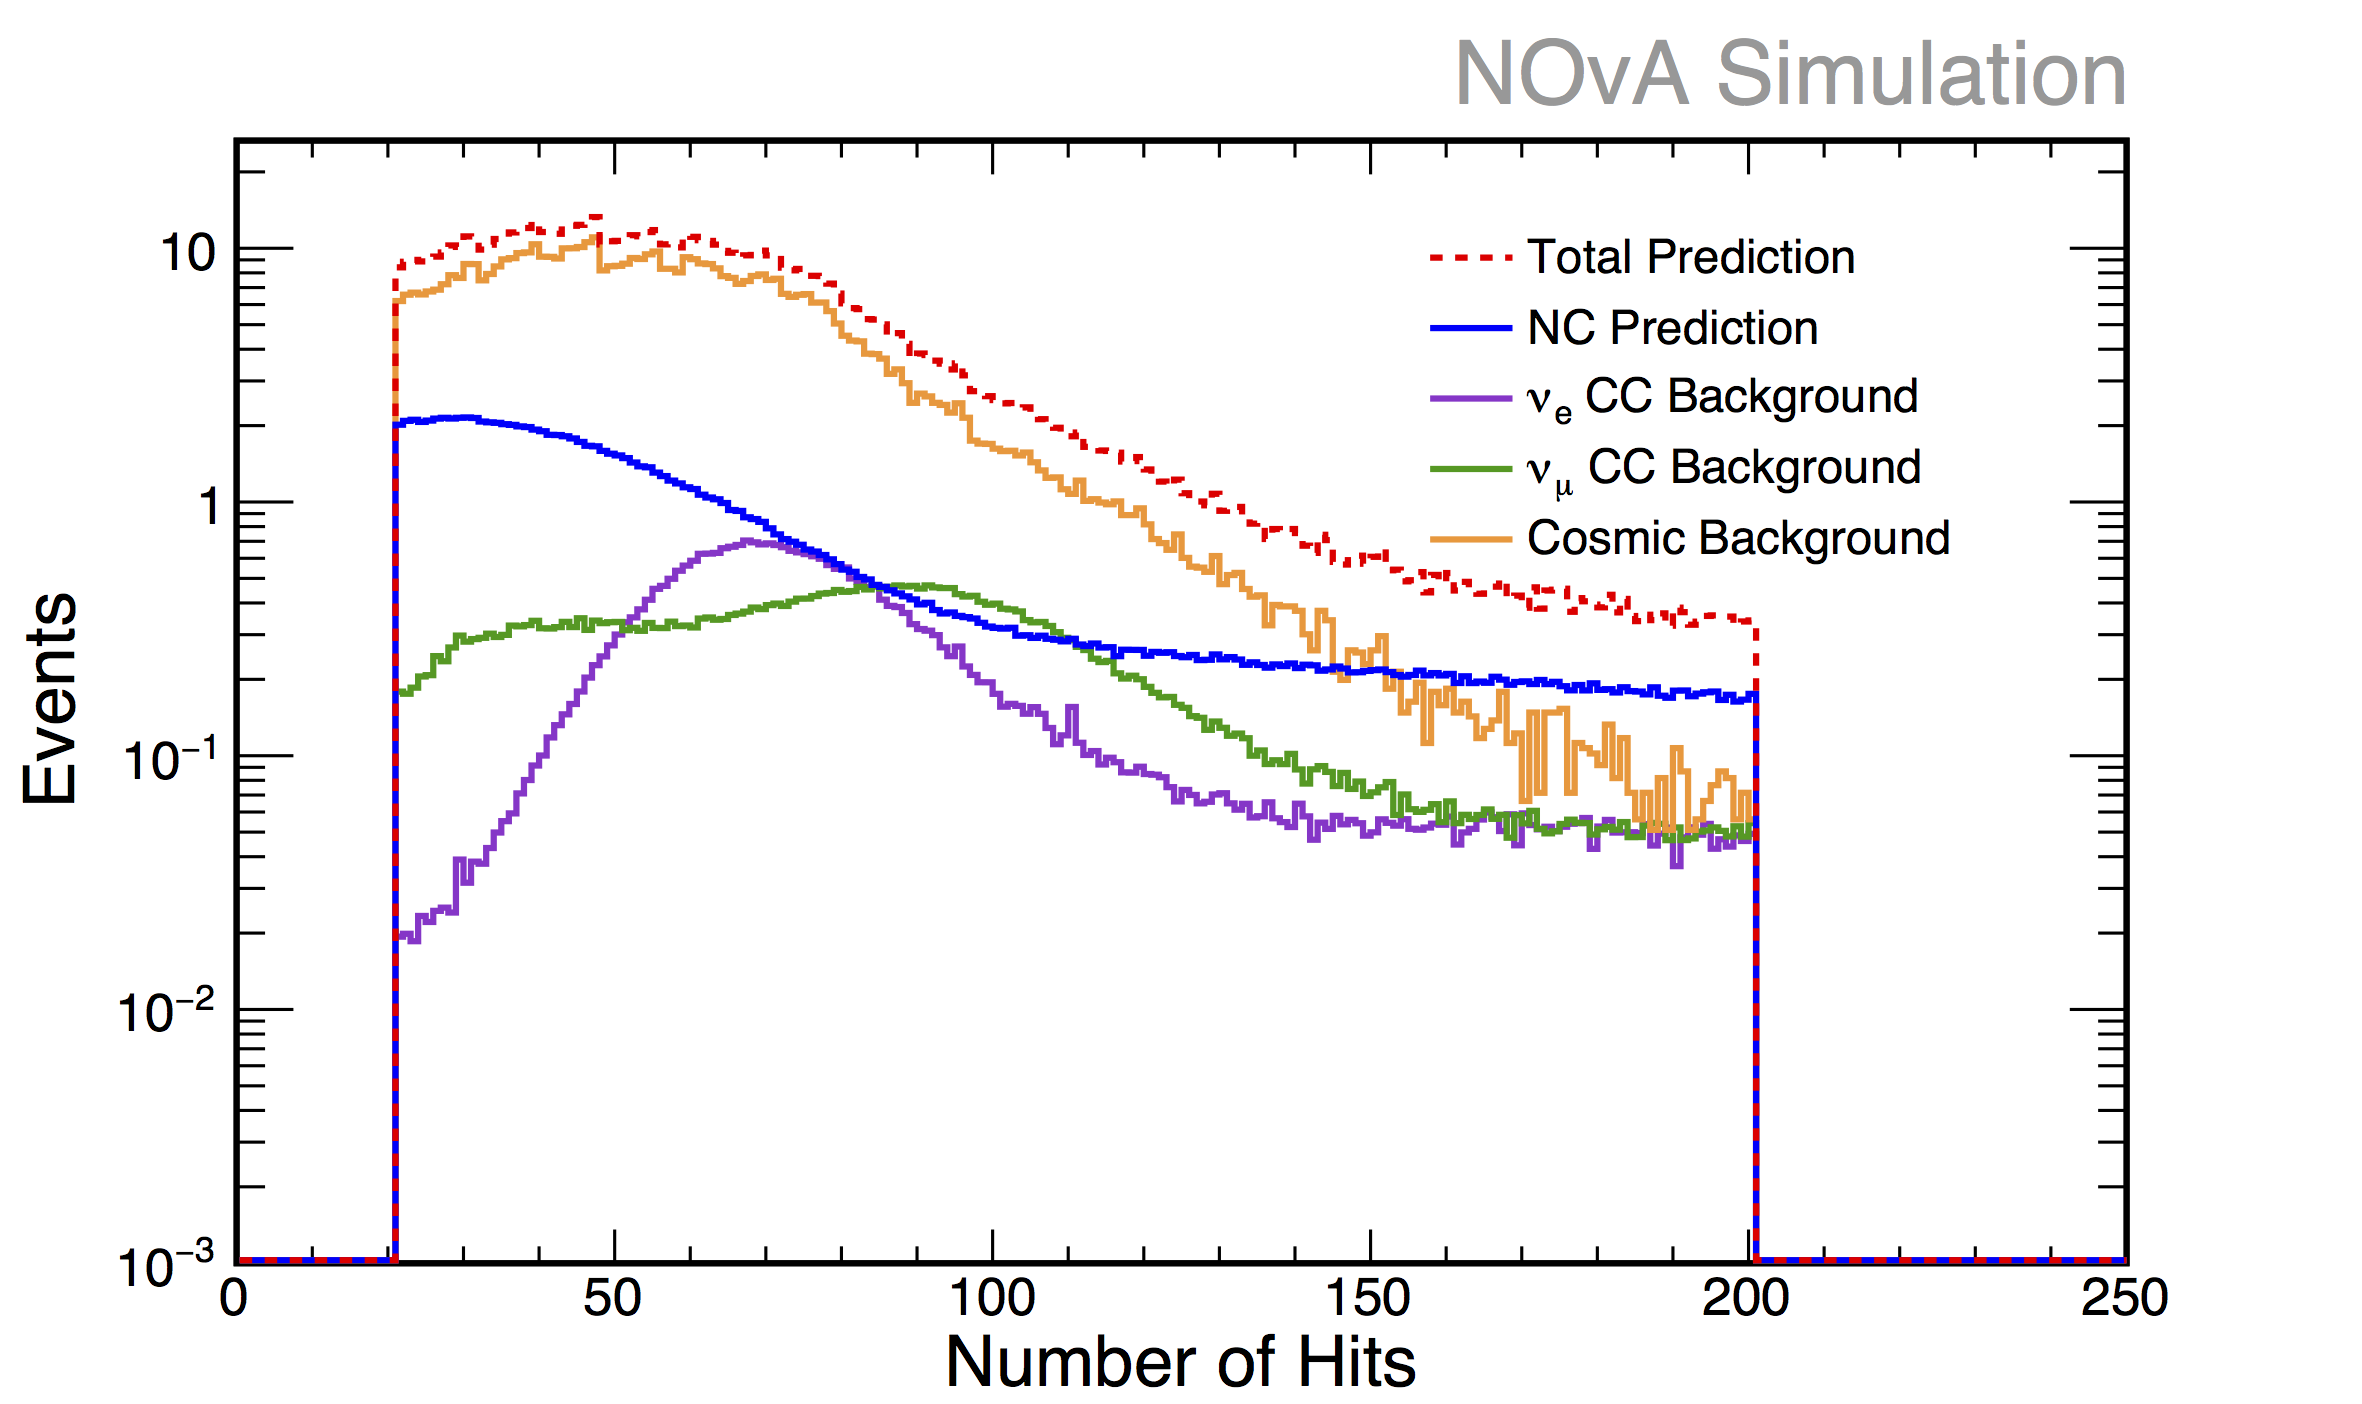
\includegraphics[width=.48\textwidth]{figures/NP1NHit.png} \\
  \end{tabular}
  \caption[Cosmic Rejection Variable Distributions]{Distributions of variables used for cosmic rejection at the FD.}
  \label{fig:CosRej}
\end{figure}

\begin{table}[h]
  \begin{center}
    \caption[Event Table: FD Cosmic Rejection Cuts]{The number of events after each cut level at the FD.}
    \label{tab:CosRej}
    \begin{tabular}{c c c c c}
      \hline\hline
      Cut Level & NC & $\numu$ CC & $\nue$ CC & Cosmic \\
      \hline
      \multicolumn{5}{l}{FD:} \\
      ...NC Selection & 113.2 & 39.7 & 31.0 & 580.0 \\
      $+$Cosmic Rejection & 94.8 & 12.1 & 7.8 & 200.0 \\
      \multicolumn{5}{l}{ND $(\times 10^{3})$:} \\
      ...NC Selection & 686.0 & 809.7 & 26.8 & \\
      $+$Cosmic Rejection & 593.5 & 360.9 & 9.7 & \\
      \hline
      \hline
    \end{tabular}
  \end{center}
\end{table}

\begin{figure}[h]
  \centering
  \begin{subfigure}{.48\textwidth}
    \centering
    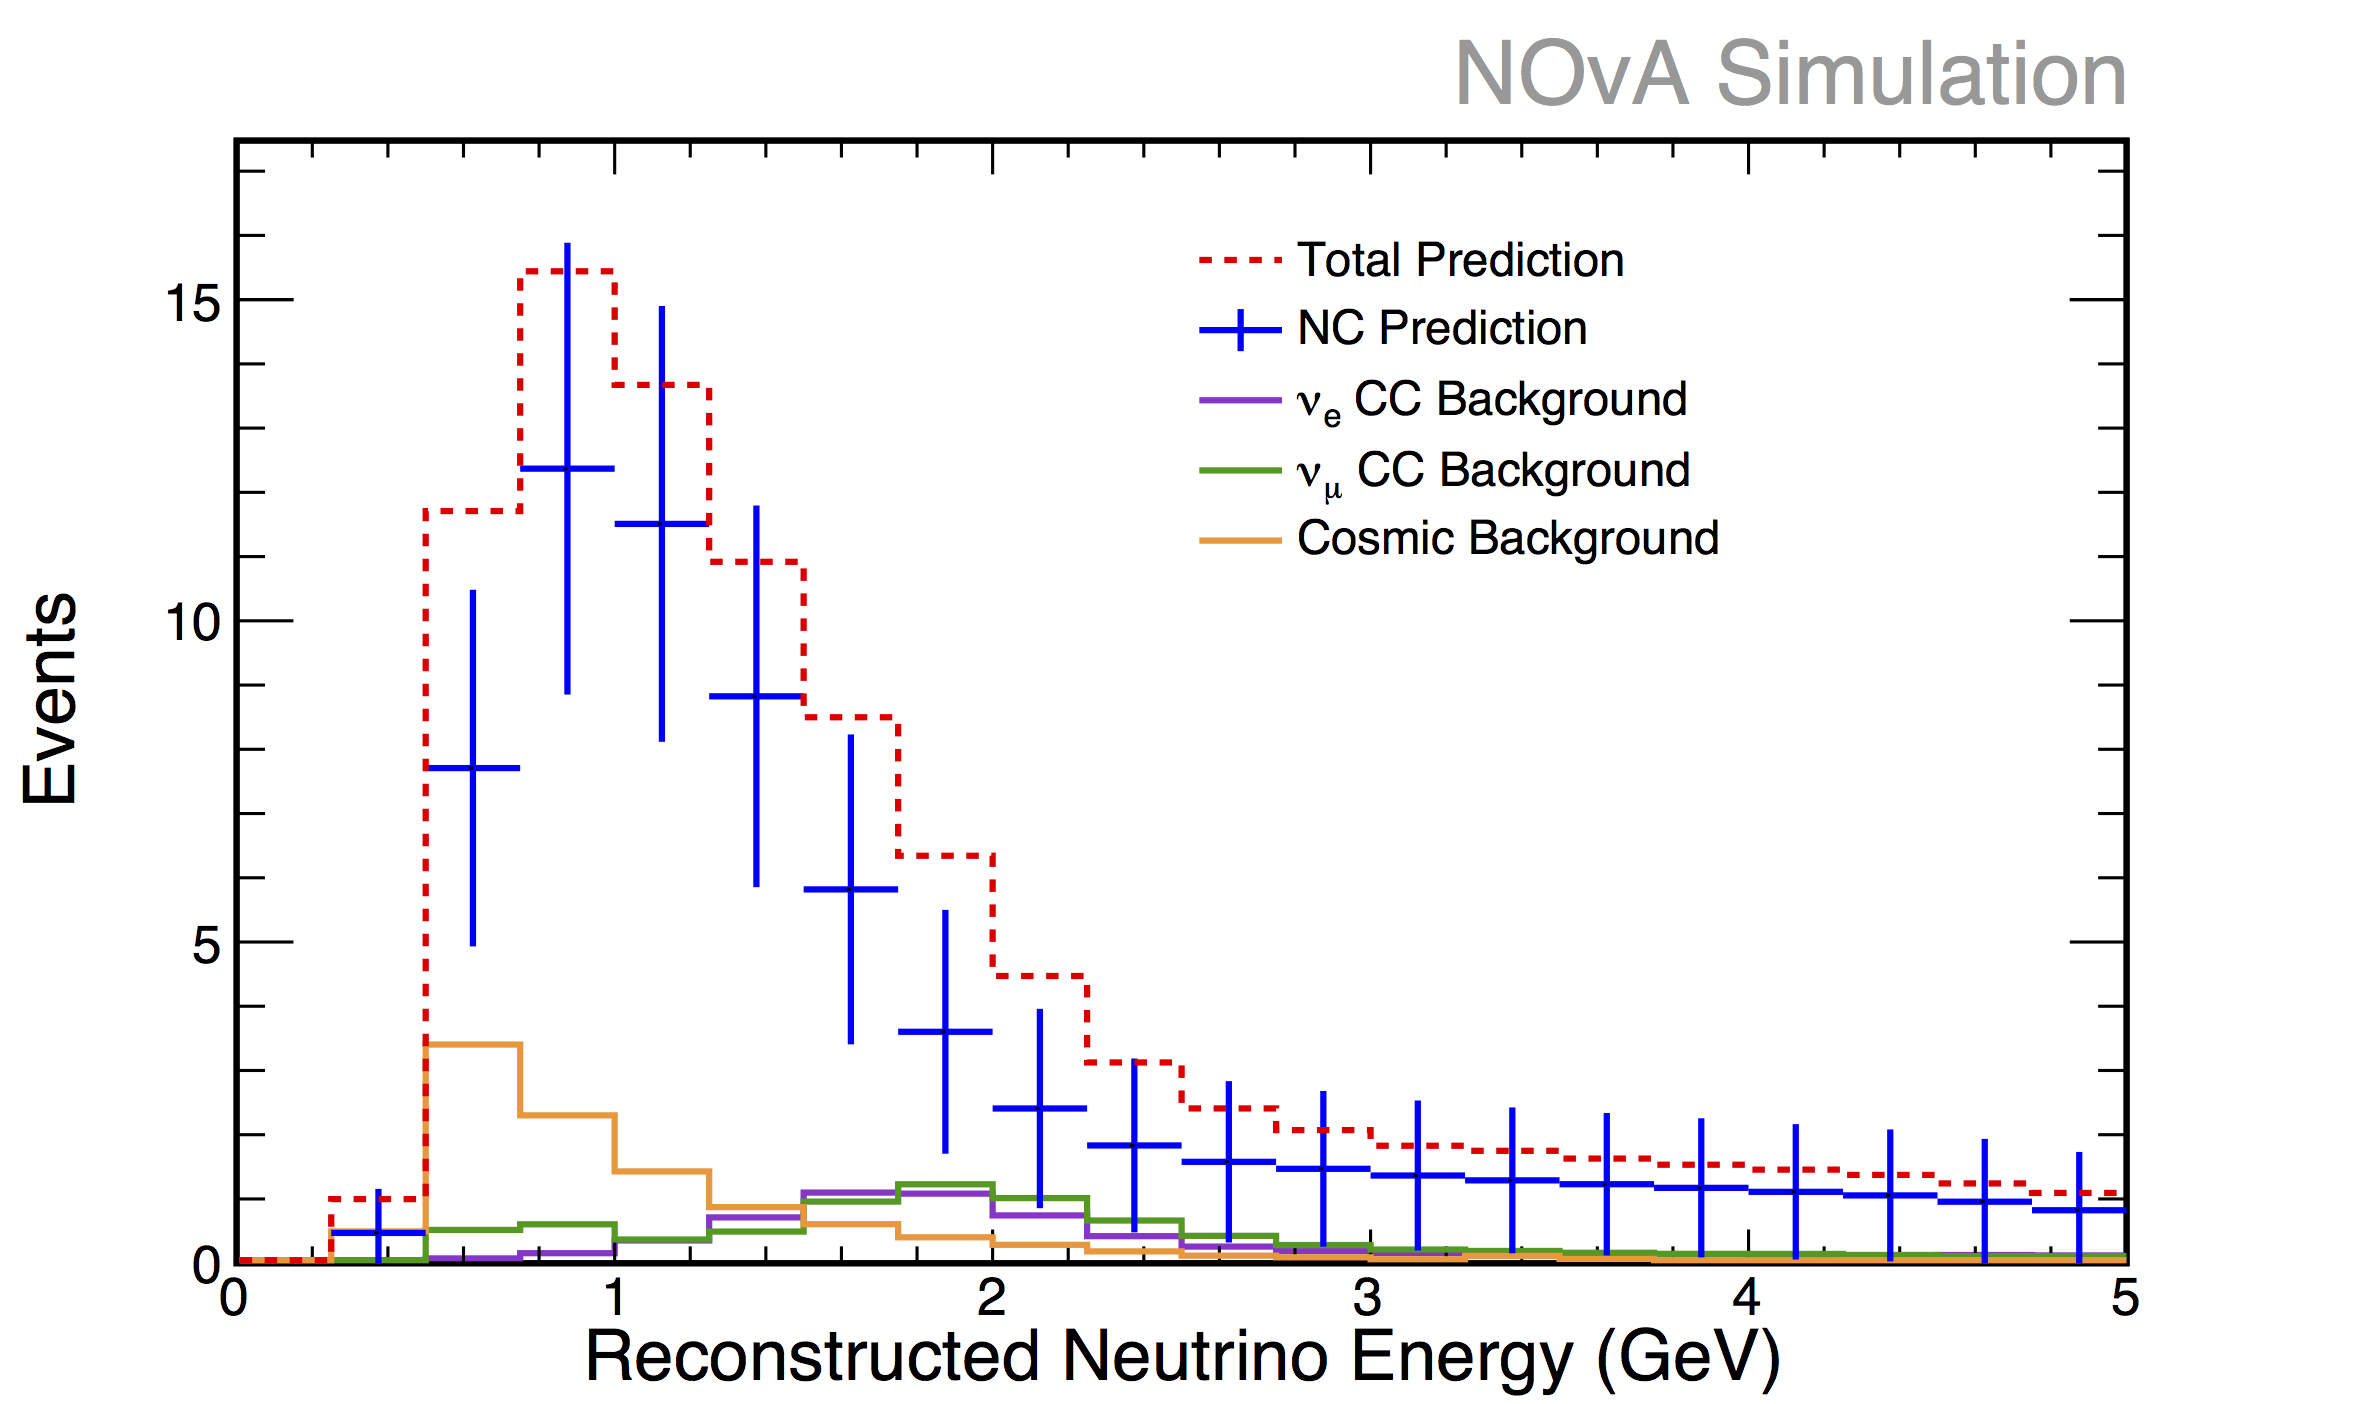
\includegraphics[width=1\linewidth]{figures/RecoE6FD.png}
  \end{subfigure}
  \begin{subfigure}{.48\textwidth}
    \centering
    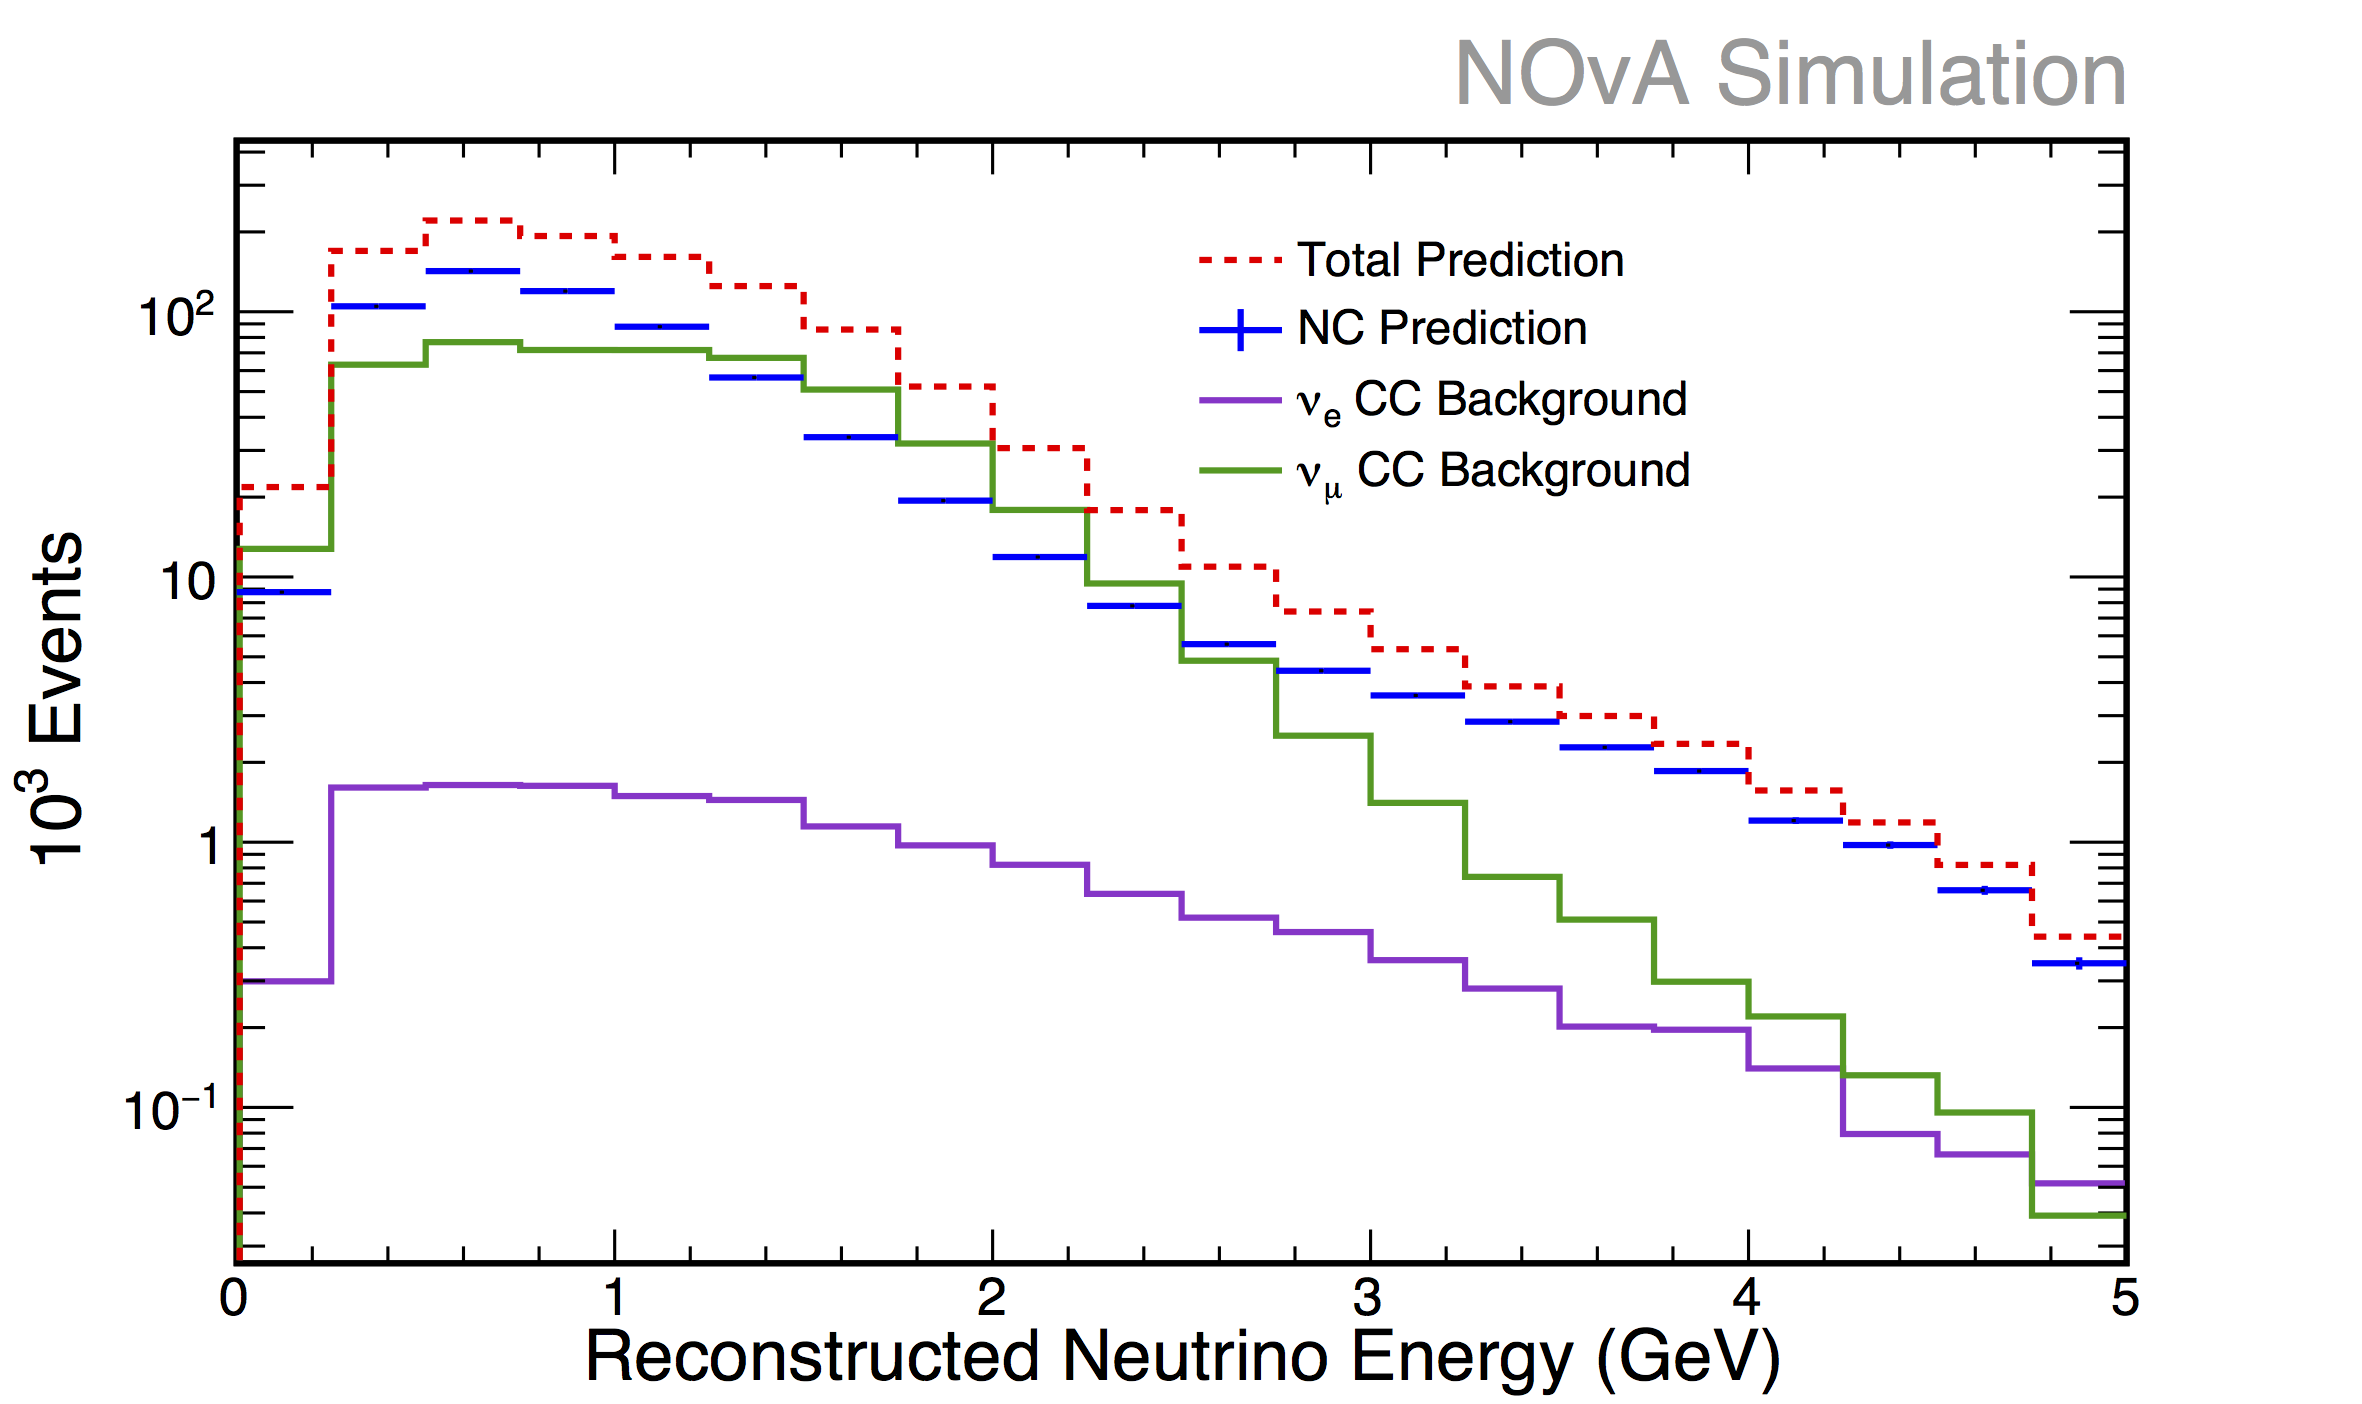
\includegraphics[width=1\linewidth]{figures/RecoE6ND.png}
  \end{subfigure}
  \caption[Energy Spectra After All Cuts]{Energy spectra after all cuts for the FD (left) and ND (right).}
  \label{fig:Sel}
\end{figure}

\section{Summary}

The final selection combines all of the cuts from the previous sections. The event rates at each level of cut are summarized for the FD in Table \ref{tab:FDSel}, and in Table \ref{tab:NDSel} for the ND. The final energy spectra are shown in fig.~\ref{fig:Sel}.
\begin{table}[h]
  \begin{center}
    \caption[Event Table: FD Selection Cuts]{The number of events after each cut level at the FD.}
    \label{tab:FDSel}
    \begin{tabular}{c c c c c}
      \hline\hline
      Cut Level & NC & $\numu$ CC & $\nue$ CC & Cosmic \\
      \hline
      Data Quality & 194.8 & 107.3 & 54.0 & 66148.4 \\
      $+$ Event Quality & 194.8 & 107.3 & 54.0 & 66148.4 \\
      $+$ Fiducial & 116.7 & 45.5 & 32.2 & 8164.7 \\
      $+$ Containment & 113.2 & 39.7 & 31.0 & 580.0 \\
      $+$ NC Selection & 94.8 & 12.1 & 7.8 & 200.0 \\
      $+$ Cosmic Rejection & 66.6 & 7.8 & 6.1 & 10.6 \\
      \hline
    \end{tabular}
  \end{center}
\end{table}

\begin{table}[h]
  \begin{center}
    \caption[Event Table: ND Selection Cuts]{The number of events after each cut level at the ND.}
    \label{tab:NDSel}
    \begin{tabular}{c c c c}
      \hline\hline
      Cut Level & NC & $\numu$ CC & $\nue$ CC \\
      \hline
      Data Quality & 3934 & 13904 & 246 \\
      $+$Event Quality & 3934 & 13904 & 246 \\
      $+$ Fiducial & 1377 & 3490 & 64 \\
      $+$ Containment & 686.0 & 809.7 & 26.8 \\
      $+$ NC Selection & 593.5 & 360.9 & 9.7 \\
      $+$ Cosmic Rejection & ? & ? & ? \\
      \hline
    \end{tabular}
  \end{center}
\end{table}